\documentclass[12pt]{article}  % <--- 12pt font
%\usepackage[margin=1in]{geometry}% <--- 1 in margin
\usepackage[papersize={8.5in,11in},margin=1in]{geometry}

\usepackage{lscape}
\usepackage{booktabs}
\usepackage{array}%[=2016-10-06]
\usepackage{tabu}
\usepackage{colortbl}

\newcolumntype{P}[1]{>{\centering\arraybackslash}m{#1}}
\usepackage{multirow,calc,amsmath}
\newlength\mylenA
\newlength\mylenB
\newlength\mylenC
\newlength\mylenD
\usepackage{tikz}
\usepackage{tcolorbox}
\usepackage{etoolbox}
\AtBeginEnvironment{tcolorbox}{\normalsize}

\usepackage{adjustbox}[valign=t]

\tcbuselibrary{skins, breakable}

\makeatletter
\tcbset{
  tabular/.style={
    boxsep=\z@,top=\z@,bottom=\z@,leftupper=\z@,rightupper=\z@,
    toptitle=1mm,bottomtitle=1mm,boxrule=0.5mm,
    fontupper=\small,
    before upper={\arrayrulecolor{tcbcolframe}\def\arraystretch{1.1}%
      \tcb@hack@currenvir\tabular{#1}},
    after upper=\endtabular\arrayrulecolor{black}},
}
\makeatother

\usepackage{color, colortbl}
\usepackage{graphicx}
%\usepackage{subfigure}
\usepackage{caption}
\usepackage{subcaption}
%\usepackage{tcolorbox}

\usepackage{amsmath}
\usepackage{amsthm}
\usepackage{dsfont}
\usepackage{statmath}
\usepackage{mathtools}
\usepackage{physics}
\usepackage{xcolor}
\usepackage{hyperref}
\usepackage{makecell}
% \usepackage{pgfplots}
% \usepackage{tikzviolinplots}
% \usepgfplotslibrary{external}
% \tikzexternalize
% \usepackage{minted}
% \usemintedstyle{gruvbox-light}
% \usepackage{scontents}


 
\newcommand{\bx}{\mathbf{x}}
\newcommand{\mD}{\mathcal{D}}
\newcommand{\mG}{\mathcal{G}}
\newcommand{\mM}{\mathcal{M}}
\newcommand{\mE}{\mathcal{E}}
\newcommand{\gray}{\rowcolor[gray]{.90}}
% Natbib setup for author-year style
\usepackage{natbib}
 \bibpunct[, ]{(}{)}{,}{a}{}{,}%
 \def\bibfont{\small}%
 \def\bibsep{\smallskipamount}%
 \def\bibhang{24pt}%
 \def\newblock{\ }%
 \def\BIBand{and}%
\def\pipeline{Explanation Pipeline}
\newcommand{\tw}[1]{\textcolor{red}{Tong: #1}}

\def\checkmark{\tikz\fill[scale=0.4](0,.35) -- (.25,0) -- (1,.7) -- (.25,.15) -- cycle;} 

\normalem

\onehalfspacing
\newtheorem{theorem}{Theorem}
\newtheorem{corollary}[theorem]{Corollary}
\newtheorem{proposition}{Proposition}
\newenvironment{proof}[1][Proof]{\noindent\textbf{#1.} }{\ \rule{0.5em}{0.5em}}

\newtheorem{hyp}{Hypothesis}
\newtheorem{subhyp}{Hypothesis}[hyp]
\renewcommand{\thesubhyp}{\thehyp\alph{subhyp}}

\newcommand{\red}[1]{{\color{red} #1}}
\newcommand{\blue}[1]{{\color{blue} #1}}

\newcolumntype{L}[1]{>{\raggedright\let\newline\\arraybackslash\hspace{0pt}}m{#1}}
\newcolumntype{C}[1]{>{\centering\let\newline\\arraybackslash\hspace{0pt}}m{#1}}
\newcolumntype{R}[1]{>{\raggedleft\let\newline\\arraybackslash\hspace{0pt}}m{#1}}

\geometry{left=1.0in,right=1.0in,top=1.0in,bottom=1.0in}

\begin{document}

\begin{titlepage}
\title{The Risk of Inferring Data Insights from Post hoc Explanations of Machine Learning Models}
\author{Ronilo Ragodos\thanks{University of Iowa} \and Tong Wang \thanks{Yale University} \and Lu Feng \thanks{University of Electronic Science and Technology of China} \and Jeffrey Hu \thanks{Purdue University}}
\date{\today}
\maketitle
\begin{abstract}
\noindent Machine learning models have been increasingly used in business research. However, most state-of-the-art machine learning models, such as deep neural networks and XGBoost, are black boxes in nature. Therefore, post hoc explainers that provide explanations for machine learning models by, for example, estimating numerical importance of the input features, have been gaining wide usage. Despite the intended use of post hoc explainers being explaining machine learning \textit{models}, we found a growing trend in business research where post hoc explanations are used to infer the importance of explanatory variables ($X$) in the \textit{data}. In this work, we investigate the validity of such use. Specifically, we investigate with extensive experiments \emph{whether} the feature importance values obtained by the two most popular post hoc explainers, SHAP and LIME, provide correct information about the true marginal effects of $X$ on $Y$ in the data, which we call data-alignment. We then identify \emph{what} factors influence the alignment of explanations. Finally, we propose a set of mitigation strategies to improve the data-alignment of explanations and demonstrate their effectiveness with real-world data in an econometric context. In spite of this effort, we nevertheless conclude that it is not appropriate to infer data insights from  post hoc explanations. We articulate appropriate alternative uses, the most important of which is to facilitate the proposition and subsequent empirical investigation of hypotheses. The ultimate goal of this paper is to caution business researchers \textit{against} translating explanations of machine learning \textit{models} into potentially false insights and understanding of \textit{data}.
\vspace{0in}\\
\noindent\textbf{Keywords:} XAI, XML, post-hoc explainers\\
\vspace{0in}\\
%\noindent\textbf{JEL Codes:} key1, key2, key3\\

\bigskip
\end{abstract}
\setcounter{page}{0}
\thispagestyle{empty}
\end{titlepage}
\pagebreak \newpage

\maketitle

% use statistics of the citation of the post hoc papers
% show how difficult it is to solve the problem, e.g., cite cynthia's paper
\section{Introduction}
    % Mention Marketing Science Institute "consistently identified attribution as a topmost research priority over the last few years" (from SHAP meets uniform paper)

% =========================== Tong ===========================
Over the past few decades, the surge in data volume and complexity has led to the widespread adoption of machine learning (ML) for business analysis \citep{kleinberg2015prediction,mullainathan17applied}. ML is commonly used in scenarios where researchers focus on predicting a particular variable of interest. This translates into formulating a supervised learning problem where the target variable is predicted by an ML model using explanatory variables (features).

However, in business research, prediction alone is often insufficient. Researchers and practitioners are also interested in gaining insights about their data through predictive ML models. In particular, they seek information about how explanatory variables are associated with the target variable, a relationship that can be described by the marginal effects of the explanatory variables\footnote{Note that marginal effects are descriptive and do not directly indicate causality.}. 
Unfortunately, most ML models with high accuracy operate as black boxes\footnote{It is worth acknowledging that recent years have seen the emergence of inherently interpretable models that can attain comparable performance to black box models, sans the reliance on post hoc explanations. However, these models, which lie beyond the purview of this paper's discussion, will not be further delved into here.} that produce predictions without providing any information about the explanatory variables. Thus, researchers often cannot obtain data insights directly from their predictive models.


In response to the opacity of black box models, post hoc explainers have naturally garnered significant attention from business researchers. Explainers provide various types of explanations of black box models, such as feature importance \citep{ribeiro16lime,lundberg17shap}, partial dependence plots \citep{friedman01pdp}, counterfactual examples \citep{mothilal20dice}, etc. Many recent business research follows what we call the Explanation Pipeline, shown in Figure \ref{fig:pipeline}, where a black box ML model is employed for a complicated prediction task and  subsequently explained by a post hoc explainer. Thus, users can gain some understanding of the model's decision-making process, such as the importance of different features. % feature importance for the ML model,  from which they draw some conclusions on the features as if they are using $\boldsymbol{\beta}$s.
Although post hoc explanations are intended to explain ML models, a growing number of researchers seem to expect that such explanations can be extrapolated to understand the underlying data for the model. This expectation is particularly pertinent for explainers that produce feature importance, such as Local Interpretable Model-Agnostic Explanations (LIME) \citep{ribeiro16lime} and Shapley Additive Explanations (SHAP) \citep{lundberg17shap}\footnote{We will only study SHAP and LIME in this paper.}.


Indeed, recent literature increasingly adopts this problematic perspective. SHAP and LIME explanations of black box models have been extrapolated in diverse areas of business literature to make inferences about the marginal effects of the features. For instance: \cite{park2024extracting} claims that SHAP explanations provide guidance on what smartphone features customers prefer. \cite{jiang24churn} says that if a customer has a large value for a feature with large SHAP values, they are more likely to be churners, and \cite{sanchez2023role} claims that their SHAP explanations reveal what factors actually drive hotel guest satisfaction and hotel managers should plan their service strategies accordingly, to name a few. Some recent work is quite optimistic about post hoc explanations - \cite{berger2023supply} advocates the use of the combination of an ML model and SHAP as an ``alternative to OLS."

To gain a deeper understanding of the prevalent practice of employing post hoc explanations in business research, we conducted a thorough review of the literature. Specifically, we meticulously examined 150 papers from the business literature published between 2018 and 2024\footnote{LIME was published in 2016, and SHAP was published in 2017. Considering the time it takes to write a business paper, we set the start time of our literature search to 2018 for papers that use either LIME or SHAP.} utilizing either SHAP or LIME. Notably, our findings reveal that among these 150 papers (109 of which are from top journals \footnote{We consider a journal a top journal if the 5-year impact factor is above 5 or the journal is an INFORMS journal. Note that SHAP and LIME are relatively new methods, and the business journal review processes are long. Therefore, many of the remaining papers are still under review and are not counted among the 109 top journal papers we reviewed.}), 42\% used explanations to draw conclusions about the relations between $X$ and $Y$ in the data, rather than in the ML model being explained. Their conclusions and supposed insights can be roughly categorized into three dominant types\footnote{There are some other incorrect uses, which we will discuss in the appendix. Further details and comprehensive results of this analysis can also be found in the online supplementary  appendix.}. First, papers make claims about the qualitative relationships between $X$ and $Y$, most commonly about whether an $X$ has a positive or negative relationship with $Y$. They use language like ``$X_j$ has a positive/negative impact on $Y$'', when the explainer provides a positive/negative feature importance for feature $X_j$. Second, papers infer the relative importance of the features from post hoc explanations. They use language like ``$X_1$ is more important to $Y$ than $X_2$ is" if the feature importance of $X_1$ is larger than that of $X_2$. Finally, some papers would use post hoc explanations to identify the most influential features and use language like ``$X_{j_1}, X_{j_2}$, and $X_{j_3}$ are the most important to $Y$" when the feature importance for $X_{j_1}, X_{j_2}$, and $X_{j_3}$ are greater in magnitude than the others. 
Such use of explainers to draw conclusions on data suggests an emerging paradigm shift in which, through post hoc explanations, ML models are used not only for prediction but also as a means to gain understanding of data. However, the validity of using explainers for this purpose remains unjustified. 


  % \citep{lorentzen2020peeking}. 
      \begin{figure}[t]
        \centering
        %\fbox{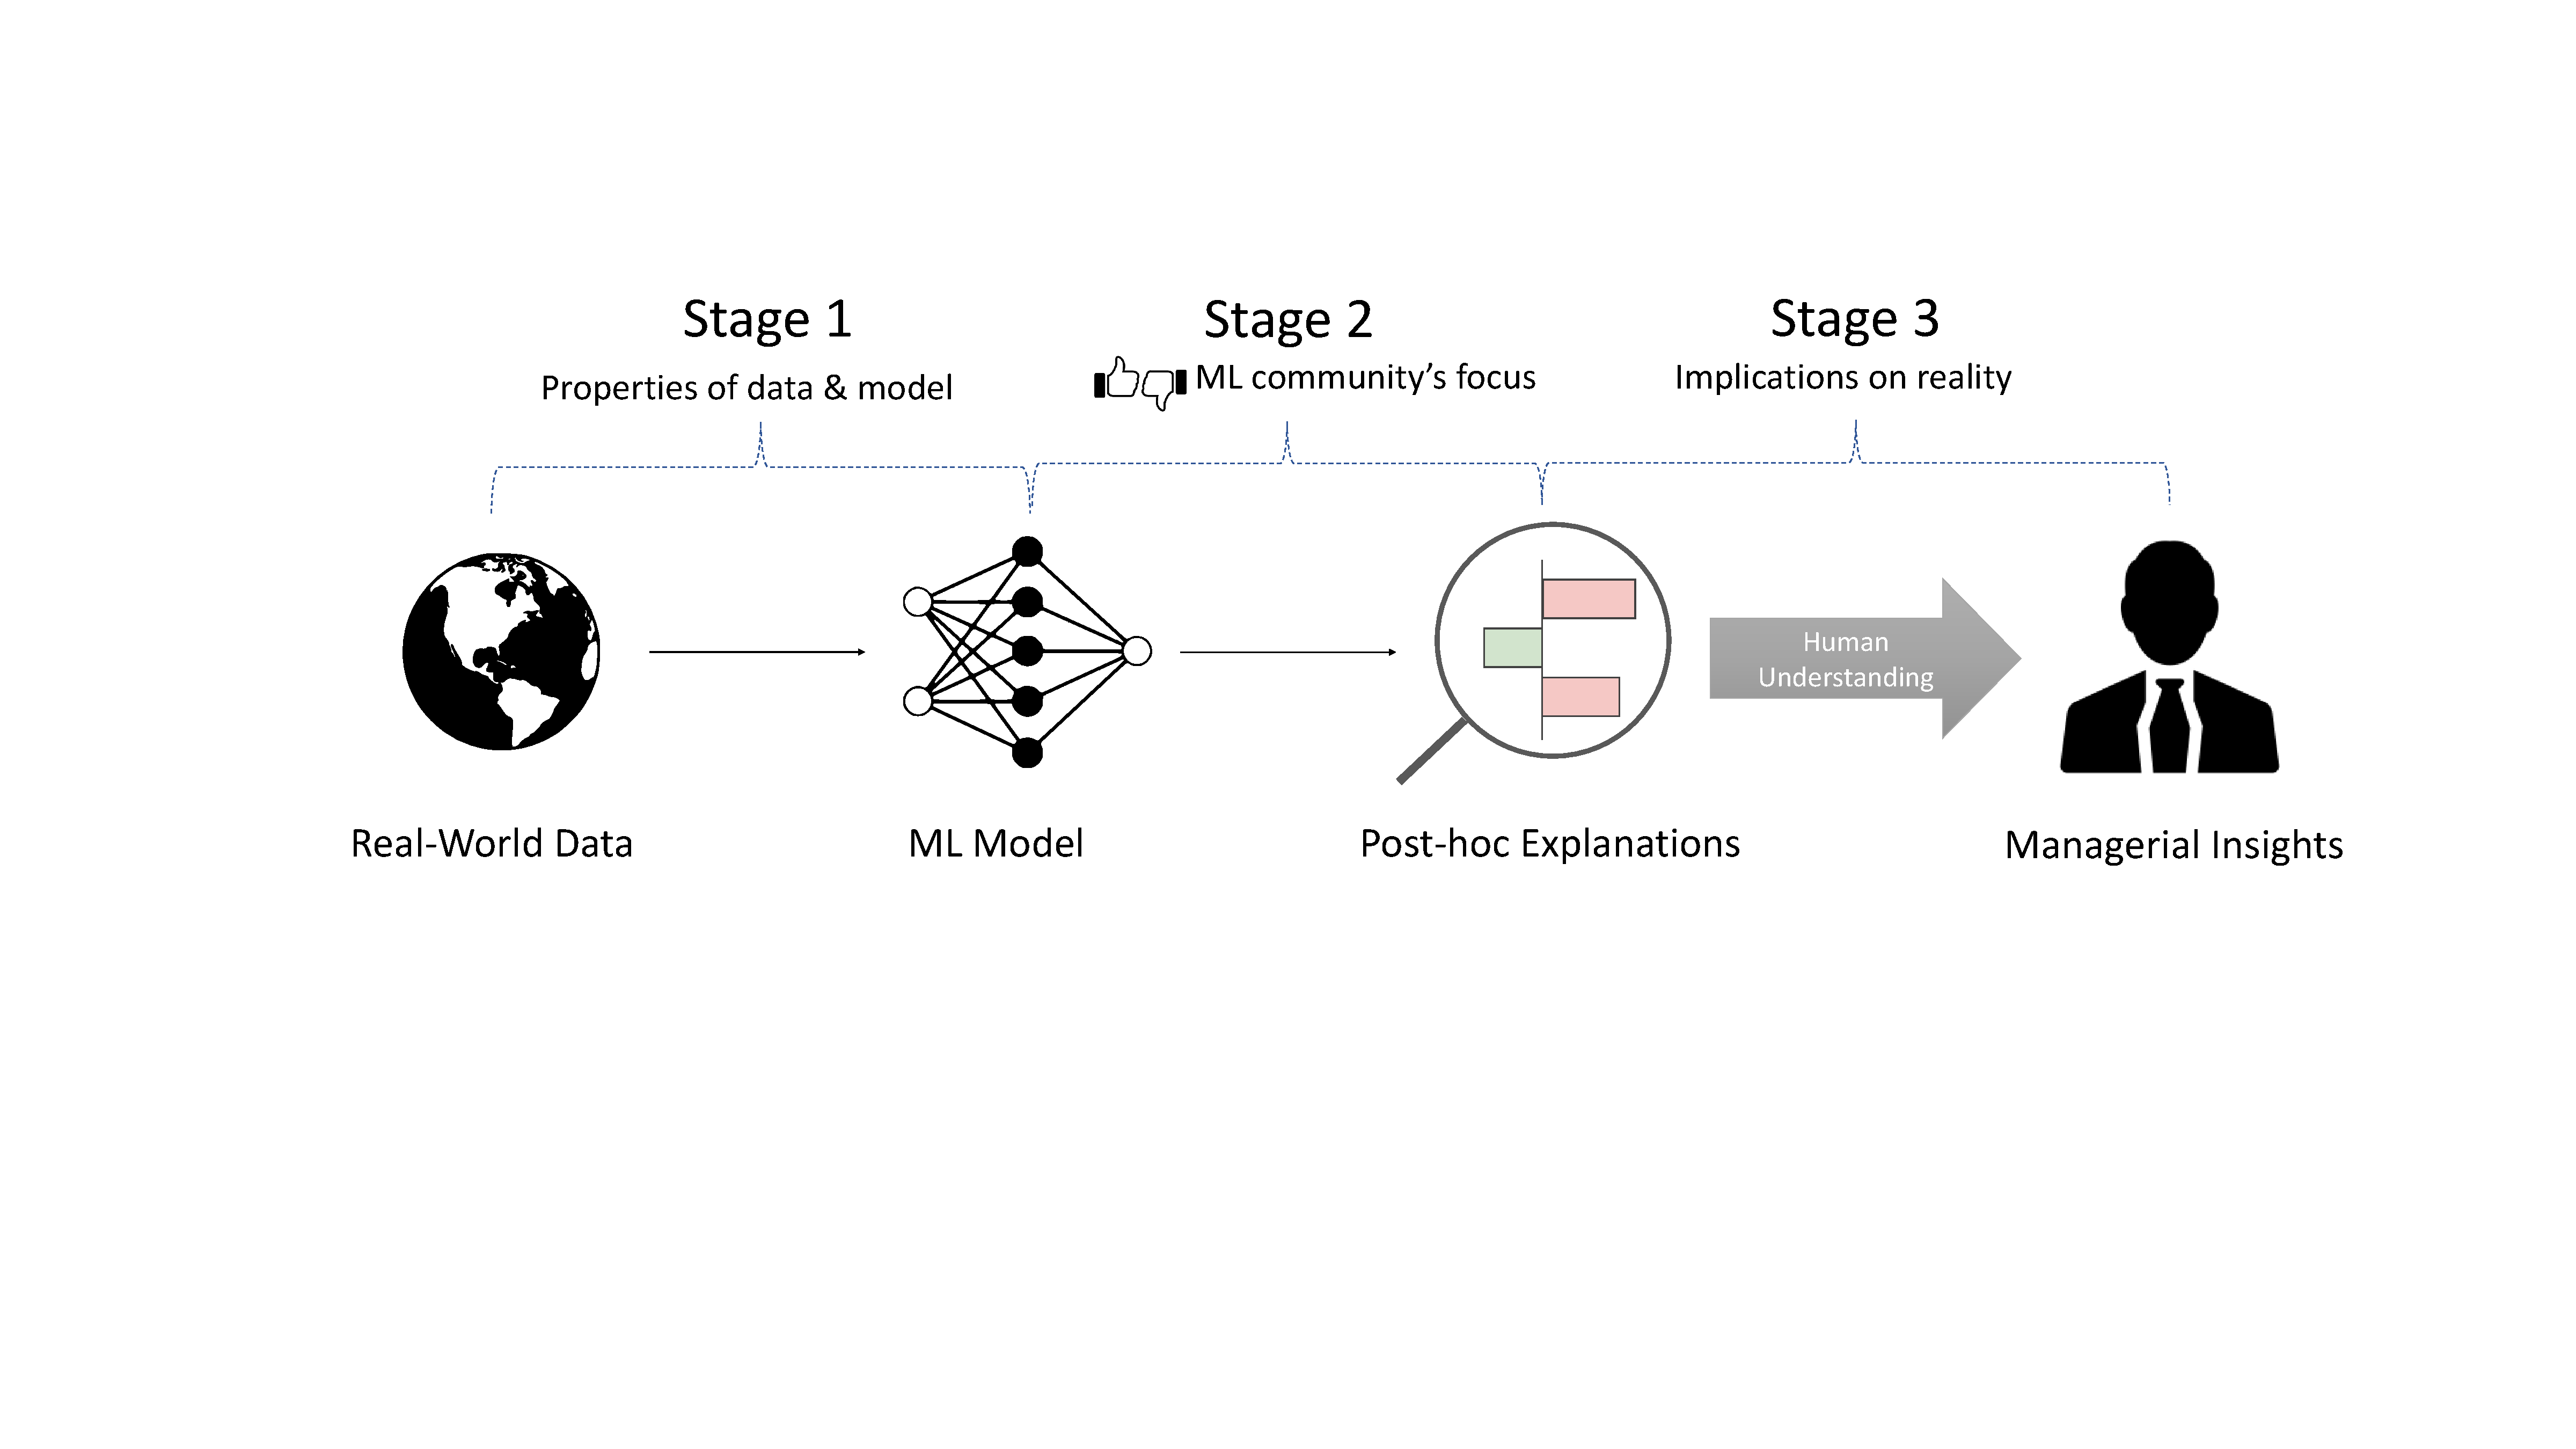
\includegraphics[width = \textwidth,trim=250 500 150 250 mm, clip=true]{Figures/pipeline.pdf}}
        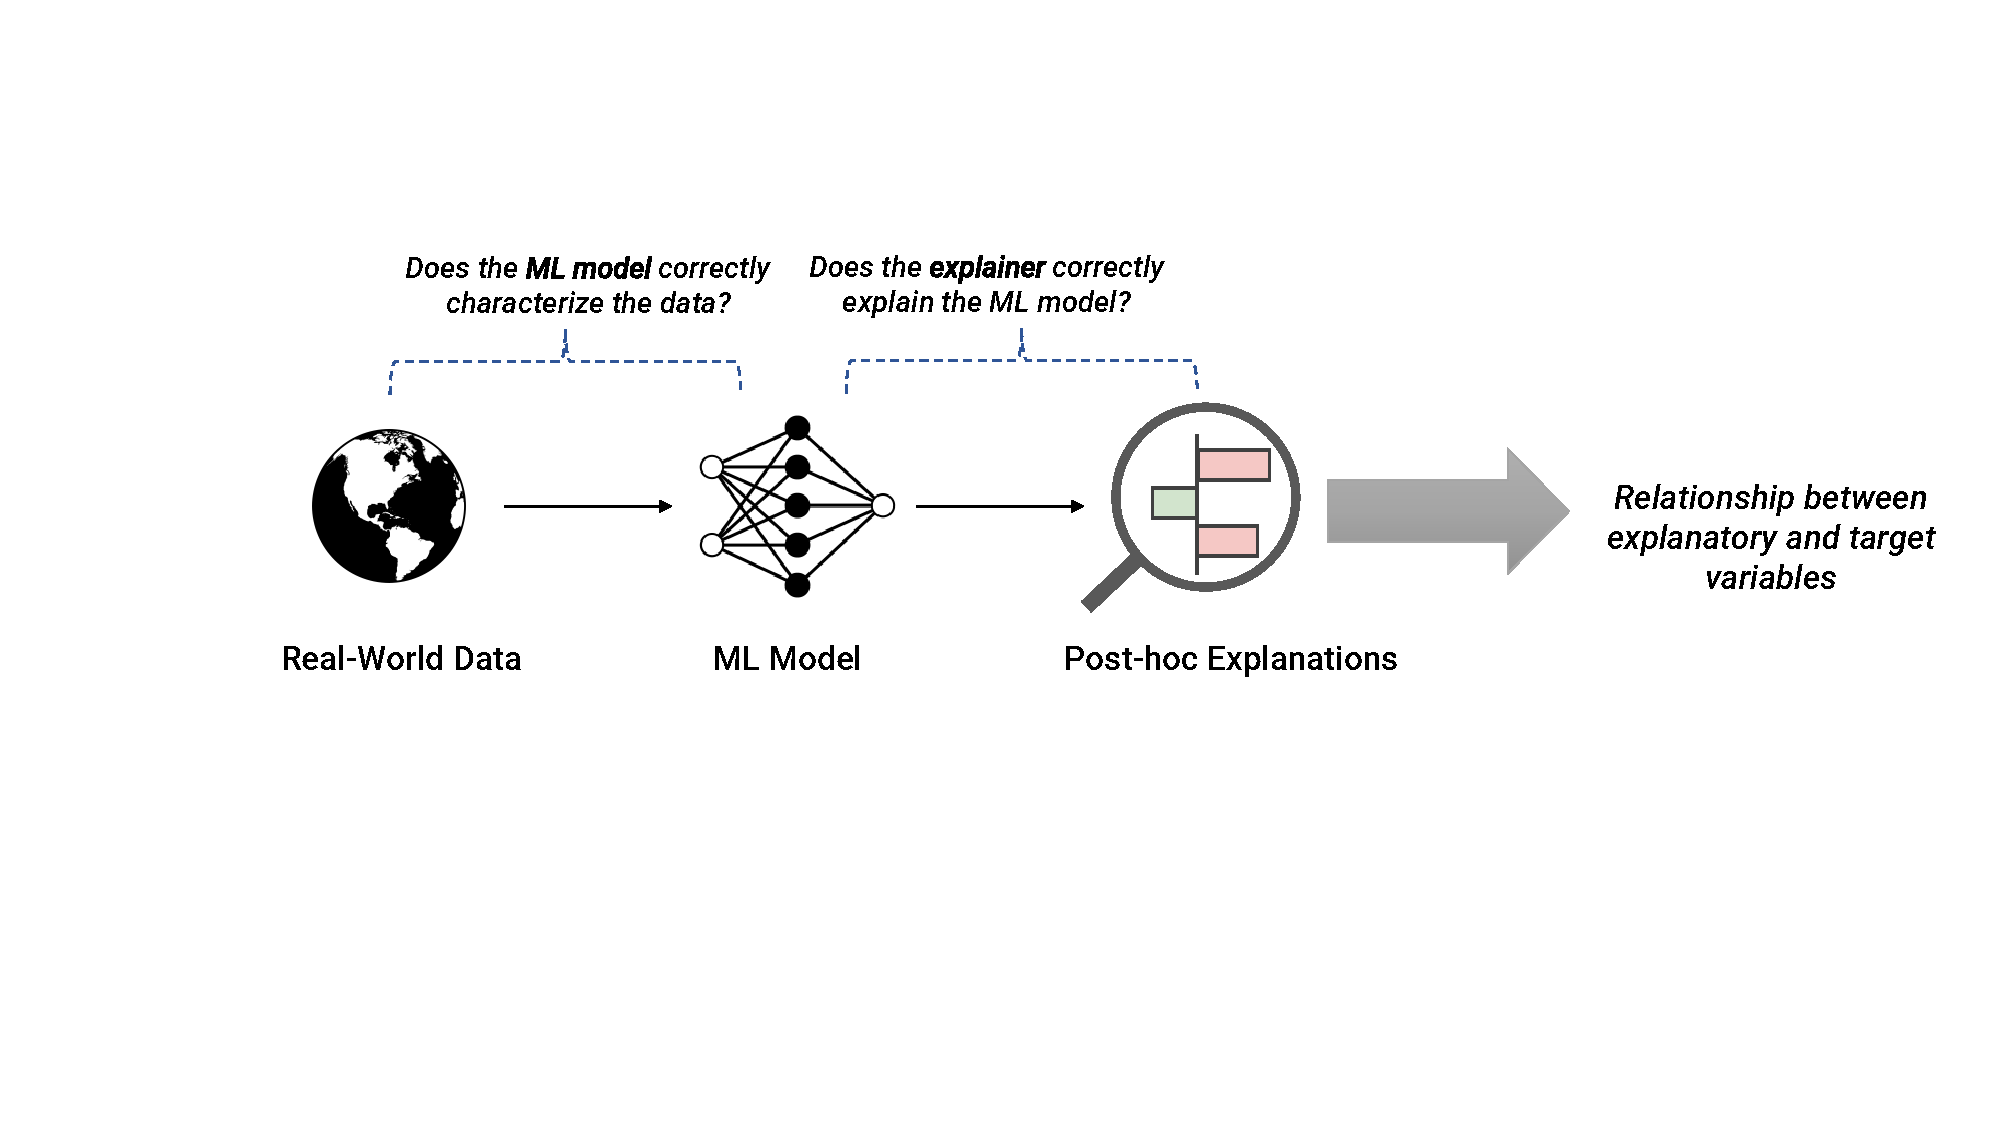
\includegraphics[trim={4.75cm 7.5cm 1.125cm 4.25cm},clip, width = 0.9\textwidth]{Figures/pipeline_flow_new.pdf}
        \caption{Explanation Pipeline: the pipeline of using post hoc explainers to explain a machine learning model. Additionally inferring information about the actual marginal effects of the features constitutes mistaken usage of the pipeline.}
        \label{fig:pipeline}
    \end{figure}
     % They build a black box ML model for a complicated task, which could have many variables, or strong interactions of variables, or include unstructured data, such that canonical econometric methods do not easily apply. Then a post hoc explainer is used to generate feature importance for the ML model,  from which they draw some conclusions on the features as if they are using $\boldsymbol{\beta}$s. 
 

 
 % In addition, there are many types of feature importance \citep{AchenChristopherH1982Iaur}. However, except for \citep{lorentzen2020peeking}, the works cited in the previous paragraph did not provide a formal definition of feature importance and justify that the explainer(s) used were actually providing that type of feature importance. Similarly, the basic question of why Shapley values are appropriate feature importance measures is never addressed in these works\footnote{It is argued in \citep{kumar20shap} that Shapley values are not conducive to human understanding of feature importance.}. 


%Therefore, the goal of this paper is to urge the research community to approach post hoc explanations with skepticism and a more critical eye. 
% We argue in this paper that there exist fundamental flaws in using post hoc explanations to elicit information on $\boldsymbol{\beta}$s. 
Therefore, the goal of this paper is to conduct a thorough investigation into this new and emerging trend of research methodology so that we might advise the business research community
against this particular inappropriate use of post hoc explainers. We aim to directly answer the question, %``\emph{Can explanations from SHAP and LIME be extrapolated to infer $X$ and $Y$ relationship in the data?}''
``\emph{Can SHAP and LIME explanations capture the correct relationship between $X$ and $Y$, specifically the marginal effect of $X$ on $Y$, in the data?}''
with both empirical and theoretical evidence.  Specifically, we investigate whether the SHAP and LIME explanations align with the true marginal effects in the data within the three contexts that they are often used in, as described previously. For this purpose, we design three \textit{new} metrics. The first evaluates whether an explanation's feature importance values have the same signs as the corresponding marginal effects. We call it the \textbf{directionality} of an explanation since it represents the direction of the feature influence. The second metric evaluates how much the ranking of features by a post hoc explanation agrees with the ranking induced by the marginal effects. We call it the \textbf{concordance} of an explanation. The last metric evaluates whether a post hoc explanation identifies the most important features. We call it the \textbf{relevance} of the explanation. These metrics assess the extent to which the explanations are consistent with the marginal effects in terms of the sign, the ranking of features, and the identification of the most important features. We call the evaluation of the three metrics the test of \textbf{data-alignment}.

We evaluate the data-alignment of post hoc explanations using simulated data where we can control the ground truth marginal effects in the data. We set our ground truth models to be linear because the extent an explainer can produce data-aligned explanations of simple linear models is  indicative of its potential for data-alignment in more general, practical scenarios. If an explainer cannot give data-aligned explanations of simple linear phenomena, it is very likely unable to explain the complex processes underlying practical datasets. Our findings reveal that SHAP and LIME explanations typically do not align with the marginal effects and the alignment further drops as the feature dimension increases. This misalignment is evident even in straightforward business scenarios with a linear ground truth model and when the black box model being explained demonstrates high predictive performance on data containing all relevant features to $Y$, all of which are mutually independent. We then delve into the causes of this misalignment, discovering that various factors within the explanation pipeline affect the explanation quality. These include having correlated features in the data, the predictive performance of the black box model, and specific settings of explainer model parameters. We corroborate the initial presentation of our results by showing that misalignment pervades an additional 100 simulations where we explain models produced using AutoML that were trained on datasets with varying numbers of features, rows, and label noise.


Critically, we offer a theoretical justification for why SHAP explanations inherently fail to align with the marginal effects, making Shapley values fundamentally inappropriate for any definite claims regarding marginal effects. We discuss in Section \ref{sec:theoretical_considerations} that SHAP estimates situational importance~\citep{StrumbeljErik2014Epma}, 
 which expresses the consequence of a feature taking on a value different from its mean. Although the computation of situational importance for a feature involves its marginal effect, the information it contributes can be destroyed in the process. Furthermore, we present theoretical grounds for conditions under which LIME might achieve a high degree of data-alignment.

% \textcolor{red}{I think we should say SHAP and LIME separately. }

% We then demonstrate another critical issue of post hoc explanations: inconsistency. Inconsistency refers to the difference in explanations produced by different configurations within the Explanation Pipeline. Using the same simulated data, we show that varying choices along this pipeline can lead to significantly divergent, and occasionally opposing, explanations. It then follows from the view that the purpose of science is to identify phenomena that occur without fail that post hoc explainers have very limited utility to researchers.


Finally, we explore potential strategies to increase the data-alignment of explanations provided by SHAP and LIME. Although our theoretical and empirical findings suggest that it is not possible to fully eliminate the issue of data-misalignment, they nevertheless reveal opportunities for improvement, which we address. For instance, for SHAP, the most immediate way to increase data-alignment is to divide its Shapley values by the differences between the corresponding feature values and their means; for LIME, increasing some hyperparameters will significantly increase the alignment with the data.

Another strategy that showed promise involves averaging the explanations derived from a family of accurate models. We also observe that when the training data used by a black box model include all relevant features, all of which are independent, the alignment of explanations of the black box's predictions with the ground truth tends to increase. This suggests that the underlying data quality and structure play a significant role in the effectiveness of post hoc explanations.
However, other intuitive strategies we tested, such as combining explanations from both SHAP and LIME for a single black box model or increasing the local approximation accuracy of LIME, did not yield effective results. This highlights the complexity of the issue and the need for more nuanced solutions.
It is also important to note that while our proposed mitigation strategies improve data-alignment to various degrees, they do not completely resolve the issue of misalignment inherent in SHAP and LIME. Consequently, post hoc explainers such as SHAP and LIME should be used with great caution by business researchers, and the appropriate uses of such tools need to be clarified.%Specifically, researchers should not rely on post hoc explanations to validate hypotheses in data. %add something about robustness/causal forest here??????


Overall, our paper identifies and cautions against a growing trend of inappropriate use of post hoc explanations to draw definite conclusions on data. We argue that post hoc explanations should not be used to \textbf{validate} hypotheses about data; instead, their role in gathering knowledge about data should be limited to \textbf{proposal} of hypotheses. To gain an accurate understanding of the underlying relationships between $X$ and $Y$ in the data, we emphasize the need for more rigorous and comprehensive follow-up analyses, both quantitatively and qualitatively. This distinction is essential to ensure the prevention of the overestimation of the reliability and validity of insights derived from post hoc explainers in business research.


    The paper is organized as follows. We will review related work pertaining to SHAP, LIME, and their weaknesses in Section \ref{sec:related_work}. Section 3 focuses on the use of SHAP and LIME in business literature, showing the prevalence of inappropriate usage. Then we use a simulated dataset with ground-truth models that we create to demonstrate the Explanation Pipeline and its vulnerabilities in Section \ref{sec:pipeline_demo}.  We provide theoretical and empirical analyses on why post hoc explanations are not suitable to infer information about marginal effects in Section \ref{sec:misalignment}. %Section 5 discusses another limitation of post hoc explanations, the inconsistency, which further hinders its use in practice. 
    We then showcase some mitigation strategies for SHAP and LIME in Section \ref{sec:mitigation_strategies} and subsequently gauge how beneficial they are over baselines in reproducing the findings of an econometric study carried out using real loan application data in Section \ref{sec:case_study}. The paper concludes in Section \ref{sec:discussion} with a summary of our findings and final remarks on post hoc explanations and their appropriate use in business research. In the appendix, we provide additional details about our experimental designs and  corroborate results of Section \ref{sec:causes_of_misalignment} by repeating the experiment on another dataset.
    
\section{Related Work}
    \label{sec:related_work}
    This section introduces SHAP and LIME and then reviews the prior literature that discusses their weaknesses. %Weaknesses discussed include intrinsic (theoretical) issues due to how the explainers are designed, and practical issues users may face due to those intrinsic issues. 

    \subsection{Post Hoc Explainers - SHAP and LIME}
     SHAP \citep{lundberg17shap} and LIME \citep{ribeiro16lime}  are the two most widely used post hoc explainers. %Model agnosticism refers to the ability to explain any ML model without the access to the internals of the ML model, i.e., only using the input and output of a model. Attributive explainers explain the predictions of a predictive ML model by attributing numerical feature importance values to each input feature. Both SHAP and LIME represent feature importance using the coefficients of an additive feature importance model. %Counterfactual explainers such as WachterCF\citep{wachter17wachtercf} and DiCE\citep{mothilal20dice} are of secondary importance and explain an output of an ML model by providing a contrasting input that cause the model to produce a different output. 
        We use SHAP and LIME as representatives for post hoc explainers in this paper because they constitute the dominant use case for post hoc explainers in business research.

        % Counterfactual explainers explain an output of an ML model by providing a contrasting input that cause the model to produce a different output. It is desirable for the contrasting input to be as close to the original as possible in order to identify a minimal change that yields a different output. Examples of counterfactual explainers include WachterCF\citep{wachter17wachtercf} and DiCE\citep{mothilal20dice}.
        
     %SHAP and LIME are model-agnostic attributive post hoc explainers. They are model-agnostic in the sense that they can explain any ML model.  Standard implementations of SHAP and LIME can explain both classification and regression models using tabular, text, or image data as input.


SHAP (SHapley Additive exPlanations) is a groundbreaking approach in the field of interpretable machine learning that offers a unified measure of feature importance. Developed by Lundberg and Lee in 2017, it builds on the concepts of game theory, particularly the Shapley value, to assign an importance value to each feature for a particular prediction. The fundamental idea behind SHAP is to assess the contribution of each feature to the difference between the actual prediction and the average prediction over the dataset. One of the unique aspects of SHAP is its consistency and local accuracy. The method guarantees that if a model changes in a way that makes a feature more important, the SHAP value of that feature will not decrease. Local accuracy ensures that the contributions of all features sum up to the actual prediction minus the average prediction, providing a detailed and accurate decomposition of the prediction. Note that LIME does not have this local accuracy property. There are several variants of SHAP, such as Kernel SHAP \citep{lundberg17shap}, TreeSHAP \citep{lundberg2018consistent} and DeepSHAP \citep{lundberg17shap}. Each variant retains the core principles of SHAP while adjusting the computational strategy to suit the specific model architecture, ensuring that the interpretability benefits of SHAP can be realized across a wide range of machine learning models.
    % SHAP's additive feature importance model differs from LIME's in that the coefficient of each feature represent the Shapley value~\citep{shapley97shapley} of that feature. SHAP surrogate models are not fit on sampled training data instances directly like LIME's, but rather on sampled coalition vectors (binary vectors indicating presence of each feature). Shapley values were originally a game-theoretic notion meant to quantify how much each player contributed to the final score of a game. In the context of SHAP, the Shapley values (surrogate model coefficients) represent how much the value of the feature to which they correspond contributes to the final value of the black box model's prediction. 

    
 % Underlying LIME explanations are ridge regressors fitted on data sampled around the input datum being explained. 
LIME is the very first model-agnostic post hoc explainer developed by \citet{ribeiro16lime}. In the default implementation of LIME by its authors, the input data are discretized and LIME trains a ridge regressor on a synthetic dataset constructed by sampling uniformly around the input datum. The coefficients of the ridge regressors indicate the importance of each feature. LIME discretizes numerical features into quartiles to avoid dealing with problems associated with differing scales of features and ensure users do not get confused when interpreting negative weights for negative valued features. The ridge regression's optimization weighs the sampled data with an exponential kernel and includes an $L_1$ (LASSO) penalty to encourage explanations to be sparse. The ridge regressors are called surrogate models because they are trained to approximate the predictions of the black box model.
    
    LIME's ridge coefficients are meant to represent marginal effects, but depending on the LIME variant and the model being explained, they are not the gradient of the black box model at the input being explained. \citet{garreau2020looking} proved that the original LIME formulation's coefficients did not, in general, equal the gradient of the black box model at the input being explained. Instead, each feature importance value is proportional to the partial derivative of the black box at the input datum and the proportionality constants differ by feature. \citet{agarwal21clime} showed that a simpler variant of LIME called C-LIME that does not discretize input features and does not perform weighted ridge regression produced coefficients that are proportional to the gradient of the black box model. %Removing discretization allows C-LIME to recover the gradient because otherwise, local information about the black box's decision boundary is destroyed.
    In discretizing features, the data used in LIME's regression problem consists of binary features indicating which bins (quantiles) the feature values of sampled data fall into, which destroys the gradient since the local information about the black box's decision boundary is lost. Moreover, C-LIME drops the ridge penalty because enforcing sparsity opposes the goal of recovering the gradient. In the specific case where the model being explained is linear, C-LIME recovers the coefficients of the linear model. This being the case, in this paper, we choose to disable the discretization setting of LIME throughout the paper to improve the quality of LIME explanations.



    \subsection{The Evaluation of Post hoc Explanations}
        \label{sec:cs_critique}
        The alarm for post hoc explanations had first gone off in the field of machine learning, as researchers questioned the correctness and validity of post hoc explanations. However, the notions of correctness and validity in the ML literature differ from the point of view we take in this paper. The ML community's attention has mainly focused on explanation quality \textbf{with respect to the ML model} since the primary goal of the machine learning field is to develop new models that make better or faster predictions. In addition, they consider factors relating the ability of humans to interpret the explanations, most of which do not fall within the scope of our critique. Thus, the way the ML community evaluates explainers is different from how we evaluate them in this paper.

    
        That post hoc explainers misrepresent the black boxes they explain is a pillar of the ML community's critique. The terms \emph{fidelity} and \emph{faithfulness} are used interchangeably and generally represent the maxims of completeness and soundness outlined by \cite{zhou21evaluating}. An explanation is complete if it is a full characterization of the black box's behavior. An explanation is sound if its characterization is correct.\footnote{In this paper, however, we characterize faithfulness in reference to the ground truth instead of the black box model because we are interested in obtaining insights about reality, not about black box models. In Section \ref{sec:evaluating_faithfulness}, we define metrics that capture our notion of faithfulness.} 
    \cite{garreau2020looking} and \cite{han22which} consider soundness from a function approximation perspective, directly measuring the difference between an explainer  and the black box model. \cite{garreau2020looking} shows that LIME's approximation error is always bounded away from 0. \cite{han22which} analyzes kernelSHAP and LIME relying on a view of KernelSHAP and LIME as kernel weighted linear regression models whose input data are sampled by perturbing the input by random noise. They remark that the choice of noise distribution made by kernelSHAP and LIME prevents them from being able to recover the gradient of linear models they explain as feature importance values. It follows that KernelSHAP and LIME cannot necessarily be expected to reliably perform their intended task of interpreting black box model behaviors. 
Other fidelity/faithfulness metrics measure particular approximation properties such as the extent to which an explainer assigns zero importance to features the model does not depend on are used as metrics in \cite{nguyen2020quantitative}. Metrics such as Deletion and Insertion metrics are based on the idea that features said to be important by an explainer should have significant effects on black box output \citep{deyoung20eraser,nguyen2020quantitative,alvarez18robustness,luss2021leveraging}. However, all previously mentioned papers study the fidelity with respect to the \textit{ML model}, rather than the data, as we do in this paper. Nevertheless, the aforementioned studies partially answer our research question. Because if a black box explainer has difficulty even being faithful to an ML model, it would be even more challenging for it to provide correct data insights.
%The underlying supposition of Deletion and Insertion metrics is that removing or adding features said to be important to a prediction by an explainer should change the prediction to change substantially \citep{deyoung20eraser,nguyen2020quantitative,alvarez18robustness,luss2021leveraging}. %Some works evaluate explainers by taking advantage of contexts where feature importance information of a model is known. \cite{blunsom2019can} evaluates explainers of a white box recurrent model by quantifying the explainers' error rates with respect to identifying important tokens in inputs. \cite{carmichael21framework} evaluates additive explainers by calculating the Jaccard index between the sets of effects present in neural networks and GAMs and the effects and associated contributions of features given by explainers for those models. 
    
  The ML community has also largely focused on other aspects of post hoc explanations, such as interpretability or understandability of the explanations. Explainers which satisfy desiderata related to interpretability should be able to provide a description of the behavior of a black box model in a form which can be easily understood by humans. For example, explanations should be simple enough to be intelligible but complex enough so that the explanation is still complete and sound. Parsimony \citep{nguyen2020quantitative} and clarity \citep{lakkaraju2017interpretable,montavon2018methods,alvarez18robustness} metrics, for example, measure the simplicity and ambiguity of explanations, respectively\footnote{We use the terminology of \cite{markus2021role} here.}. \cite{jacovi2023diagnosing} further requires that the form of explanations match what the psychology literature identifies as natural for human understanding.  Simplicity of explanations beyond the per-feature importance values given by attributive explainers is not desirable in our application because, e.g. artificial enforcement of sparsity could encourage explanations to omit information about the marginal effects and become incomplete and unsound as a result. For example, LIME's use of a LASSO penalty to make its explanations sparse is undesirable because it could cause a feature to have zero importance when the $\beta_j$ for that feature is non-zero. %Futhermore, stability metrics quantify how different explanations of nearby inputs are. The size of the local Lipschitz constant of the function underlying the explainer is one such example \citep{alvarez18robustness}. Stable explanations can be desirable because an explainer's explanations for two similar inputs being very dissimilar could engender mistrust of the explainer or arouse unwarranted suspicion of unfairness in the underlying decision process. These factors, however, are not within the scope of our discussion.

    
   
    
    
    \section{Use of SHAP and LIME in Business Research}
% \textcolor{red}{find papers that use post hoc explanation to get insights that resemble $\boldsymbol{\beta}$ (explaining G). Also mention that some papers only use post hoc explainer on M. It is the intended use of the post hoc explanations, but even that faces severe criticism from the ML community discusses explanations for M}

% \textcolor{red}{Move the appendix here}
        As part of our literature review process, we cataloged papers at the intersection of business and explainable machine learning. We used Web of Science and SSRN\footnote{We searched on SSRN because business journal papers usually take a few years to get published so there are many preprints available on SSRN.} to search for publications citing at least one of LIME~\citep{ribeiro16lime} or SHAP~\citep{lundberg17shap} and have either ``LIME" or ``SHAP" appear in the body of the paper. The results were filtered by topics related to business, such as management, economics, supply chain \& logistics, operations research \& management science, etc. We also identified papers published in any of the INFORMS journals in the same manner. We then iterated through up to a thousand resulting papers one by one, collecting papers that actually used SHAP or LIME to explain a machine learning model (many papers only mentioned SHAP or LIME in the contexts of related work or future work) until we had a total of 150 different papers. Out of these papers, 91\% used SHAP and 14\% used LIME to generate explanations for their models, including 5\% using both of them.

        
        We took a close look at these papers and characterized their use of post hoc explanations by the following procedure. We first searched for evidence that it was understood that the intended use of SHAP and LIME is to explain model outputs (rather than the data). We identified problematic language indicative of inappropriate use of post hoc explanations and recorded quotations of problematic sentences.
        Not all papers contained such language; in some papers it was clear or made explicit that authors used SHAP and LIME only within the scope of model explanation. Having identified any quotations which we deemed problematic, we then divided the papers into three categories: the \textit{controversial} papers that clearly extrapolated explanations to glean information about the marginal effects, the \textit{ambiguous} papers whose wording could suggest extrapolation, and the \textit{proper} papers that only used explanations for model interpretation (the intended use).% Note again, though, that both SHAP and LIME fall short for their indented purpose and face intense scrutiny from the ML community \cite{kumar20shap,garreau2020looking}.

%\textcolor{red}{add a summary of the findings \&statistics from the 116 papers}
%\textcolor{red}{double check and update the numbers}
        We found that 42\% of the papers are controversial - they clearly extrapolated explanations to gain insight into the marginal effects in the data. In addition to that, there is another 15\% ambiguous papers that at least used unclear language such that readers could interpret their findings as being made about the marginal effects. This means that \textbf{more than half} of the papers we sampled had some problematic language. Further, 76\% of the controversial papers were from top journals\footnote{A journal was considered a ``top journal" if it is an INFORMS journal or its most recent 5-year impact factor according to Clarivate's Journal Citation Reports (JCR) was at least 5.0 at the time of writing (June 2024).}.
        %Given the popularity of SHAP and the idea that the presence of this problem in publications from top journal is indicative of the pervasiveness of the problem, we also separately surveyed papers from the INFORMS family of journals that used SHAP to explain a machine learning model. About 25\% of these papers had clear extrapolations, and 17\% could be construed as having extrapolated. Thus it was still the case that about half of the papers using SHAP contained problematic language.
        We believe that this result is representative of a rising trend of using SHAP or LIME to gain data insights.

        The interpretation of SHAP and LIME feature importance values in the controversial papers fell into three categories: 1) identifying the directionality of impact of each feature (i.e., feature importance sign), 2) ranking features by relative importance, and 3) identifying a subset of the most important features. Table \ref{tab:metric_examples} below records prototypical ways in which authors expressed their desire to perform these tasks. In Section \ref{sec:evaluating_faithfulness}, we define metrics to characterize the ability of an explainer to perform these tasks. We call them directionality, concordance, and relevance, respectively. 

% ANONYMIZED VERSION
% \begin{table}[htbp]
% \small
% \caption{Correspondence Between Paper Language and Our Metrics. Statements appearing in angle braces $\langle \cdot \rangle$ 
% are meant to make the statements more general. The $X_j$ represent data features and $Y$ represents the outcome of interest.}
% \begin{tabu} to 1\linewidth {  P{3cm} | X[l,m]  }
% \toprule
% \textsc{Purpose} & \textsc{Examples} \\
% \hline
% \textbf{Identifying How Features Impact the Target (Directionality)}
% & ``...Positive SHAP values indicate that the variable has a facilitative effect on $\langle Y\rangle$, while negative values indicate a suppressive effect..." \\ 
% & \vspace{-.8cm}``...Individuals whose predictions received larger SHAP values for this feature are more likely to have $\langle Y=1\rangle$..."\\
% & ``...Choosing features with positive mean SHAP are recommended options because they have positive effects on $\langle Y\rangle$..." \\
% \hline
% \textbf{Ranking the Features by Relative Importance (Concordance)}
% & ``...This study provides insights for planning the design of $\langle X\rangle$ by assessing the relative importance and associated rankings of the $\langle X_j\rangle$ in predicting $\langle Y\rangle$..."\\\smallskip
% & \vspace{-1.3cm}``...The use of Shapley values enables us to identify and rank relevant $\langle X_j\rangle$ for the investigated $\langle Y\rangle$.."\\\smallskip
% & \vspace{-.7cm}``...Our feature rankings and visualizations of impact patterns provide policy makers with evidence for strategies to improve $\langle Y\rangle$..." \\
% \hline
% \textbf{Identifying the Most Important (Top-$k$) Features (Relevance)\hspace{3cm}}
% & ``...That $\langle X_1$, $X_2$, and $X_3\rangle$ have the top-3 SHAP values and that their SHAP values are positive reveals that increasing $\langle X_1$, $X_2$, and $X_3\rangle$ would lead to larger $\langle Y\rangle$..."\\\smallskip
% & \vspace{-.8cm}``...We use SHAP explanations of an XGBoost Classifier to identify the key features which contributing to the risk $\langle Y\rangle$..."\\\smallskip
% & ``...By using XAI to identify the most important factors and indicators that contribute to $\langle Y\rangle$, their values and fluctuations can then be monitored over time..." \\
% \hline
% \textbf{Other Usage}
% & (\textbf{OLS Alternative}) ``...The combination of a black box algorithm and SHAP provides similar economic insights as provided by pooled OLS..."\\\smallskip
% & (\textbf{Theory Confirmation}) ``...SHAP is used to interpret the quantitative associations found by XGBoost; our results provide empirical support for prior theoretical findings..."\\\smallskip
% & (\textbf{Recourse Advocacy}) ``...Since $\langle X_1$, $X_2$, and $X_3\rangle$ have high SHAP importance and substantial effects on $\langle Y\rangle$, $\langle X_1$, $X_2$, and $X_3\rangle$ should be given attention by policy makers to increase $\langle X_1$, $X_2$, and $X_3\rangle$..." \\
% \bottomrule
% \end{tabu}
% \label{tab:metric_examples}
% \end{table}


\begin{table}[htbp]
\small
\caption{Correspondence Between Paper Language and Our Metrics. Statements appearing in angle braces $\langle \cdot \rangle$ 
are meant to make the statements more general. The $X_j$ represent data features and $Y$ represents the outcome of interest.}
\begin{tabu} to 1\linewidth {  P{3cm} | X[l,m]  }
\toprule
\textsc{Purpose} & \textsc{Examples} \\
\hline
\textbf{Identifying How Features Impact the Target (Directionality)} & \makecell[l]{$\bullet$ ``...Positive SHAP values indicate that the variable has a facilitative effect \\ on $\langle Y\rangle$, while negative values indicate a suppressive effect..." \\ 
$\bullet$ ``...Individuals whose predictions received larger SHAP values for this \\ feature are more likely to have $\langle Y=1\rangle$..."\\
$\bullet$ ``...Choosing features with positive mean SHAP are recommended options \\ because they have positive effects on $\langle Y\rangle$..." \\} \\ \hline
\textbf{Ranking the Features by Relative Importance (Concordance)}
& \makecell[l]{$\bullet$ ``...This study provides insights for planning the design of $\langle X\rangle$ by \\ assessing  the relative importance and associated rankings of the $\langle X_j\rangle$ in \\predicting   $\langle Y\rangle$..."
\\$\bullet$ ``...The use of Shapley values enables us to identify and rank relevant $\langle X_j\rangle$ \\for the investigated $\langle Y\rangle$..."
\\$\bullet$ ``...Our feature rankings and visualizations of impact patterns provide \\policy makers with evidence for strategies to improve $\langle Y\rangle$..."} \\ \hline
\textbf{Identifying the Most Important (Top-$k$) Features (Relevance)}
& \makecell[l]{$\bullet$ ``...That $\langle X_1$, $X_2$, and $X_3\rangle$ have the top-3 SHAP values and that their  \\SHAP values are positive reveals that increasing $\langle X_1$, $X_2$, and $X_3\rangle$ would \\ lead to larger $\langle Y\rangle$..."\\
$\bullet$ ``...We use SHAP explanations of an XGBoost Classifier to identify the \\ key features which contributing to the risk $\langle Y\rangle$..."\\
$\bullet$ ``...By using XAI to identify the most important factors and indicators \\ that contribute to $\langle Y\rangle$, their values and fluctuations can then be monitored \\ over time..."} \\
\hline
\textbf{Other Usage}
 & \makecell[l]{(\textbf{OLS Alternative}) $\bullet$ ``...The combination of a black box algorithm and \\SHAP provides similar economic insights as provided by pooled OLS..." \\
 (\textbf{Theory Confirmation}) $\bullet$ ``...SHAP is used to interpret the quantitative \\associations found by XGBoost; our results provide empirical support  for \\ prior theoretical findings..." \\
(\textbf{Recourse Advocacy}) $\bullet$ ``...Since $\langle X_1$, $X_2$, and $X_3\rangle$ have high SHAP \\importance and substantial effects on $\langle Y\rangle$, $\langle X_1$, $X_2$, and $X_3\rangle$ should be \\ given attention by  policy makers to increase $\langle X_1$, $X_2$, and $X_3\rangle$..."} \\
\bottomrule
\end{tabu}
\label{tab:metric_examples}
\end{table}



\section{Explanation Pipeline}
    \label{sec:pipeline_demo}
    In this section, we formulate a pipeline called the Explanation Pipeline that many papers using post hoc explainers follow to obtain explanations and then use a simulated dataset to demonstrate the pipeline.
    
An explanation pipeline consists of two stages. In the first stage, which we call the \emph{prediction stage}, a machine learning model $\mathcal{M}$ is trained on data $\mathcal{D}$. This stage addresses the prediction problem, with the resulting predictions evaluated using various metrics such as accuracy, ROC, and others, which are often the primary results in many business papers that solve a prediction task. In the second stage, which we call the \emph{explanation stage}, an explainer model (e.g., LIME or SHAP), denoted by $\mathcal{E}$, is applied to $\mathcal{M}$ to generate explanations. We denote an explanation for feature $X_j$ of $\mathcal{E}$'s prediction for the $i^{\text{th}}$ data instance $\mathbf{x}^{(i)}$ as $e_{\mathcal{E}}(x^{(i)}_j)$. This stage provides model interpretation through simple human understandable explanations such as feature importance. % We will also use the notation $\mathbf{x}^{(i)}$ to represent test set instance $i$. % building a machine learning
    
    We illustrate the Explanation Pipeline with a simulated loan approval dataset\footnote{Real datasets are less suitable for the experiments in this paper because we require access to the ground truth in order to evaluate the faithfulness of the post hoc explanations. However, in Section \ref{sec:case_study}, we will conduct a case study using a real loan application dataset and use the results of a published econometric study using that dataset as the ground truth}. Our simulation models the task of predicting whether an individual will be approved for a loan based on their demographic features and credit-related features. We define a model for generating the target variable so that the ground truth is known and controllable. We also define the ground truth model to be linear, such that the explanation task is relatively easier for the post hoc explainers. %Some of the features are not independent. We demonstrate in Section \ref{sec:role_of_correlation} that the lack of feature independence effects data-alignment. This being the case, we test our mitigation strategies in Section \ref{sec:mitigation_strategies} using a variant of the data generation process where all features are mutually independent in order to control for the effect of feature correlation and focus on the effect of our mitigations.                                       
    In the following, we will describe how we generate our data and then apply the pipeline to a sample dataset using SHAP. For consistency, we will be using this dataset and its variant in Section 5. %until Section \ref{sec:role_of_correlation}, where we introduce a variant of the dataset which has only mutually independent features and used thereafter. %For example, in section \ref{sec:stage_2}, we will add confounding features to see how model explanations are affected by data that do not satisfy conditions for causal inference. Below, we show the different stages of our Explanation Pipeline.

 \subsection{Data Generation Process}
 \label{sec:data_generation}
 % \paragraph{Data Generator $\mathcal{G}$}
 %In this section, we will introduce a simulated dataset, variants of which will be used throughout the paper.  
 % thus the coefficients in the linear model are used for the ground truth. %The ground truth model is linear, so we can evaluate local explanations with respect to the ground truth's global explanation. 
 Our data generation process simulates a process of deciding whether loan applications are approved in a real-world scenario. The applicants have a total of ten features: four demographic features and six credit-related features. Table \ref{tab:simulated} summarizes how each feature is generated. % We also include an unobserved confounder to enhance the realism of the dataset - this feature is used to generate the label but not observed by $\mathcal{M}$. % The meanings and manners of construction of all the features are reported in Table \ref{tab:simulated}. 
 The credit score feature is generated based on a partial FICO credit scoring model \citep{ligons_fico} and is given by the following formula: $\text{Credit score}= 650 + (10 + 2.5\cdot \text{Credit history}) + (70 - 15 \cdot \text{Inquiries}) + (35 - 4 \cdot \text{Delinquencies}) + (105 - 100 \cdot \text{Utilization})$.  ``Cosigner" is positively correlated with ''Married: in that the probability of having a cosigner is given by $\sigma(2\cdot \text{Married} + 1 + \epsilon)$ where $\epsilon \sim \mathcal{N}(0,\frac{1}{2})$. 
\begin{table}[h]
\centering
\resizebox{\textwidth}{!}{%
\begin{tabular}{l|l|l}
\toprule
\textsc{Feature} & \textsc{Meaning}                           & \textsc{Formula}       \\ \toprule
Age              & Applicant Age                                   & Uniform(18,100)        \\ 
Sex              & Applicant Sex                                   & Bernoulli(.5)          \\
Married          & Applicant Marital Status                        & Bernoulli(.5)          \\ 
Income           & Applicant Income                                & Normal(40,000, 30,000) \\ 
Inquiries        & Number of credit inquiries                      & Uniform(0,6)           \\ 
Cosigner         & Indicator of presence of loan cosigner & Function of Married         \\ 
Utilization      & Proportion of total credit utilized            & Uniform(0,1)           \\ 
Delinquencies    & Number of delinquent  payments in last 2 years & Uniform(0,24)          \\ 
Credit Score     & Credit score based on FICO scoring & FICO credit scoring model  \citep{ligons_fico}            \\ \bottomrule
\end{tabular}%
}
\caption{Description of features for simulated loan data.}
\label{tab:simulated}
\end{table}


  % As aforementioned, we designed the underlying true model $\mathcal{G}$ that determines whether individuals are approved for a loan. The decision is based on all features but the unobserved social support feature. Social support is an unobserved confounder of ``Cosigner". In subsequent sections, we will adapt the dataset depending on what is needed for each experiment. In one experiment, for example, we will compare what happens to explainers when their dataset does and does not have an unobserved feature. 

   We define a model $\mathcal{G}$ for generating applicants' labels, \textit{approved}, or \textit{rejected}, so that we have a ground truth model that we can use to evaluate the quality of explanations from the explainers. This ground truth model represents the underlying decision-making process that is never observed.  We define $\mathcal{G}$ as a linear model and then compose it with a logistic sigmoid function to generate the labels. The true marginal effects $\boldsymbol{\beta}$ are defined using $\mathcal{G}$\footnote{Note, however, that under our definition of marginal effects, the coefficients in $\mathcal{G}$ can differ from $\boldsymbol{\beta}$ because the $\beta_j$ for a feature which influences other features is defined to be the total derivative of the response with respect to that feature.}; it is the ground truth we compare the feature importance values provided by SHAP and LIME against.
   
    $\mathcal{G}$ is defined as the following linear model taking standardized features as input. 
    % \textcolor{red}{$\mathcal{G}$ has to use all features somewhere in the paper, if not section 3 then section 4 and 5 for demonstrating some issues. If there are features in Table 2 not used by G ever, remove it}
    %\begin{tcolorbox}%[title = Ground Truth Model $\mathcal{G}$]
    \begin{equation}
    \label{eqn:gt}
    \begin{split}
    \mathcal{G}(X) =2.5 +.0005\cdot\text{Age} -0\cdot\text{Sex} +.1 \cdot \text{Married} + .25\cdot \text{Cosigner} + 1.5 \cdot \text{Credit History} + \\   3 \cdot \text{Income} - 1\cdot\text{Utilization} -.75 \cdot \text{Delinquencies} - .5\cdot\text{Inquiries} + 5.\cdot\text{Credit Score} + \epsilon
    \end{split}
    \end{equation}
    %\end{tcolorbox}
    \noindent where $\epsilon \sim \mathcal{N}(0,\frac{1}{4})$ captures all the variation in the response variable that is not explained by the explanatory variables.
    Using the logistic sigmoid function $\sigma(\cdot)$, we assign $Y = 1$ (approved) for cases with $\sigma(\mathcal{G}(\mathbf{x}))\geq 0.5$, and $Y = 0$ (rejected) otherwise. The intercept term $2.5$ is chosen so that at a baseline when feature values are zero (features are standardized, so the means of numerical features are zero), an applicant is most likely accepted. The remaining coefficients are chosen so that ``Credit Score" is the most important feature, followed by ``Credit Inquiries," ``Delinquencies," ``Income," ``Credit History," ``Married," ``Cosigner," ``Age" and finally ``Sex." These coefficients are motivated by the literature. The probability of being approved for a loan increases insignificantly with an applicant's age \citep{cfb_age}, but significantly with their credit score. The probability decreases significantly as applicants use higher proportions of their available credit and receive recent credit inquiries. The sex of a customer is not supposed to effect approval outcomes~\citep{Calcagnini2014}. 
   We then create a dataset $\mathcal{D}$ with 5000 data points by sampling from the distributions of features to simulate applicant profiles ($\mathbf{X}$) and using $\mathcal{G}$ to create the labels ($Y$).  
   In the following, we apply the Explanation Pipeline to demonstrate how one obtains a post hoc explanation by explaining $\mathcal{M}$ using $\mathcal{E}$. 


\subsection{Applying the Explanation Pipeline}
\label{sec:applying_to_simulated}
The Explanation Pipeline consists of two stages, the \emph{prediction stage} in which an ML model $\mathcal{M}$ is built using $\mathcal{D}$, and the \emph{explanation stage} in which outputs of $\mathcal{M}$ are explained with an explainer $\mathcal{E}$. 

To demonstrate the pipeline, we choose $\mathcal{M}$ to be a neural network with 100 hidden layer nodes. We perform a standard 80-20 train-test split of the 5000 applicants. The accuracy of $\mathcal{M}$ is 0.86 and the AUROC is 0.93 on the test set. We choose $\mathcal{E}$ to be SHAP for demonstration purpose since SHAP is used a lot more often than LIME. %Unless otherwise stated later in the paper, this model is what $\mathcal{M}$ refers to. 
%Then we use SHAP to explain $\mathcal{M}$'s decision on one applicant.% in hopes of learning about the marginal effects underlying the data, i.e., the coefficients in $\mathcal{G}$.% We do not allow LIME to discretize the input features to give it a better chance of recovering $\boldsymbol{\beta}$ (recall from Section \ref{sec:related_work} the comparison of default LIME and C-LIME)\footnote{We show in the Appendix that allowing discretization makes LIME's results demonstrably worse.}. %Since LIME builds a linear model locally for the focal instance being explained, the coefficients of LIME's linear model and the ground-truth coefficients can be compared to evaluate how faithful LIME is to the ground truth.
We demonstrate the explanation of SHAP using one applicant that we will call John. John is a 61-year-old married male who makes approximately \$66,000/year, has a credit score of 761, 6 credit inquiries in the past 6 months, and utilizes 19\% of his 28-month old line of credit. He also has a cosigner and no delinquent payments in the last two years. John's application was accepted, that is, $Y = 1$. Since we design the data generation model $\mathcal{G}$, we know the ground truth marginal effect of each feature in obtaining John's application outcome, following formula (\ref{eqn:gt}). John's feature values along with SHAP's explanation for his approval are visualized in Figure \ref{box}. We denote them by $e_\text{SHAP}(x_j)$. %For the most part, it was because their credit score is too low. We will now see if LIME can produce this insight.

 % \begin{figure}[ht!]
 %     \centering
 %     \includegraphics[width=.48\textwidth]{Figures/shap_ex.png}
 %     \caption{}
 %     \label{fig:shap_ex}
 % \end{figure}
\settowidth\mylenC{\textbf{$\mathcal{M}=\text{\textbf{XGBoost}}$}} 
% determine usable width of cols 2 and 3:
\setlength\mylenD{(.3\linewidth-3\tabcolsep)/3}
    \begin{figure}[ht!]
    \small
        \centering
            \begin{subfigure}[t]{.35\textwidth}
              \centering
              %\includegraphics[height=.5\linewidth]{Figures/shap_ex_feat.png}%}%{Figures/feng_fig/acc_increase_iter_2.png}
                \begin{tabular}[b]{l|l}
                \toprule
                \textbf{Feature} & \textbf{Value} \\ \hline
                Credit Score     & 761            \\
                Income           & \$66,000       \\
                Credit History   & 28 months      \\
                Cosigner         & Yes            \\
                Married          & Yes            \\
                Age              & 61             \\
                Sex              & Male \\
                Inquiries        & 6              \\
                Delinquency      & 0              \\
                Utilization      & 19\%           \\
                \bottomrule
                \end{tabular}
              \caption{John's feature values}
              \label{fig:shap_ex_feat}
            \end{subfigure}%
            \hfill%#space{1cm}
            \begin{subfigure}[t]{.6\textwidth}
              \centering
\begin{tcolorbox}[tabular = {*{6}{wc{\mylenD}}}, hbox,center,label = {pipelines_3_ex}]
\\%\midrule
\noalign{\vspace{-\normalbaselineskip}}
\multicolumn{3}{c}{\textsc{$\mathcal{G}$}} & \multicolumn{3}{c}{\textsc{Pipeline: }$\mathcal{M}=\text{\textsc{NN}}$}  %& \multicolumn{3}{c}{\textsc{Pipeline 2: }$\mathcal{M}=\text{\textsc{XGBoost}}$} 
\tabularnewline \cmidrule(lr){1-3}\cmidrule(lr){4-6}%\cmidrule(lr){7-9}
\multicolumn{3}{c}{\textsc{Ground Truth}} & \multicolumn{1}{wc{\mylenD}}{$\mathcal{E}$} & \multicolumn{1}{wc{\mylenD}}{\textsc{Accuracy}} & \multicolumn{1}{wc{\mylenD}}{\textsc{AUC}}\tabularnewline%\midrule
\multicolumn{3}{c}{} & \multicolumn{1}{wc{\mylenD}}{\textsc{SHAP}} & \multicolumn{1}{wc{\mylenD}}{$.86$} & \multicolumn{1}{wc{\mylenD}}{$.93$}\tabularnewline\midrule
%\multicolumn{3}{c}{\textsc{Ground Truth}} && &%\multicolumn{1}{c}{$\mathcal{E}$} & \multicolumn{1}{c}{\textsc{Accuracy}} & \multicolumn{1}{c}{\textsc{AUC}} %& \multicolumn{1}{wc{\mylenD}}{$\mathcal{E}$} &\multicolumn{1}{wc{\mylenD}}{\textsc{Accuracy}} & \multicolumn{1}{wc{\mylenD}}{\textsc{AUC}}\tabularnewline\midrule
 %& & & \multicolumn{1}{wc{\mylenD}}{SHAP} &\multicolumn{1}{wc{\mylenD}}{.86} & \multicolumn{1}{wc{\mylenD}}{.93} %& \multicolumn{1}{wc{\mylenD}}{SHAP} &\multicolumn{1}{wc{\mylenD}}{.86} & \multicolumn{1}{wc{\mylenD}}{.97}\tabularnewline %\midrule
\multicolumn{3}{c|}{\begin{minipage}{.45\textwidth}
      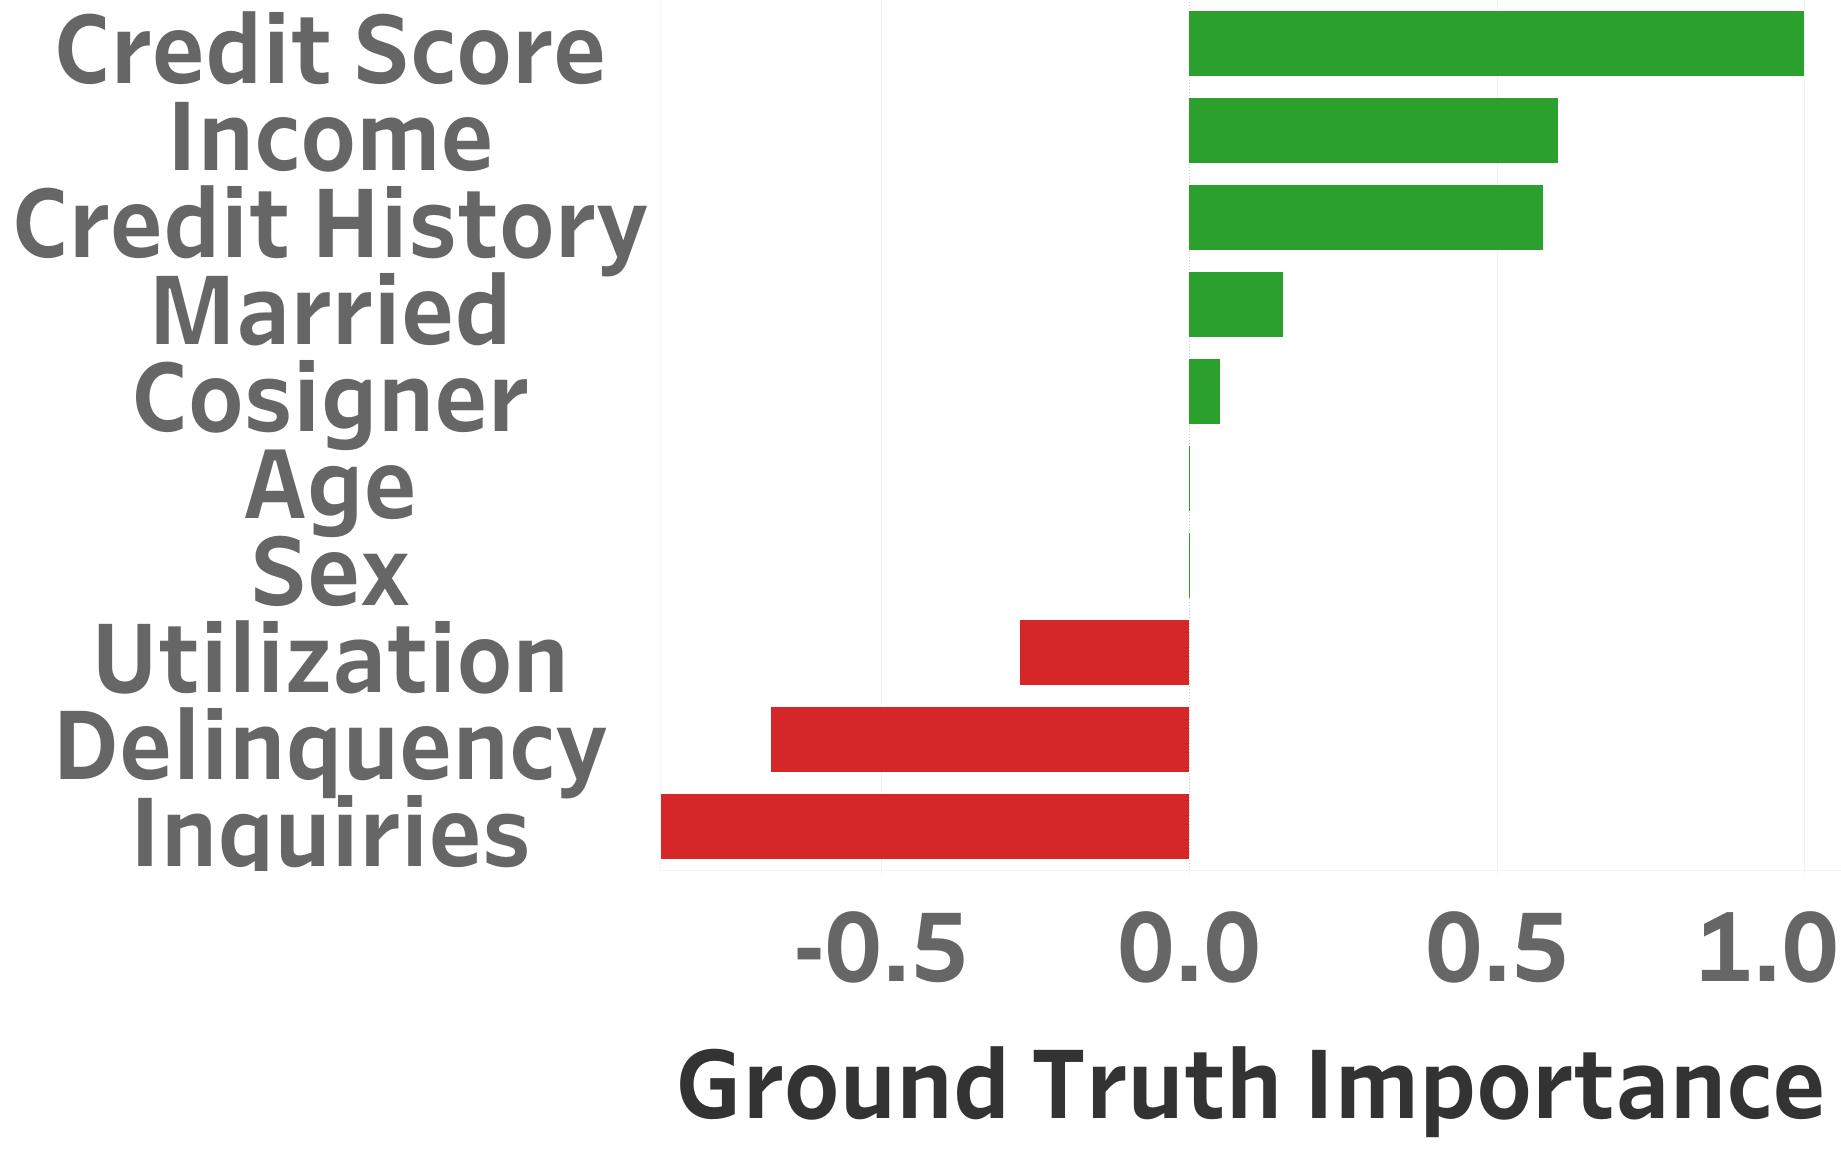
\includegraphics[width=\linewidth]{Figs/g_ex.png}
    \end{minipage}} & \multicolumn{3}{c}{\begin{minipage}{.45\textwidth}
      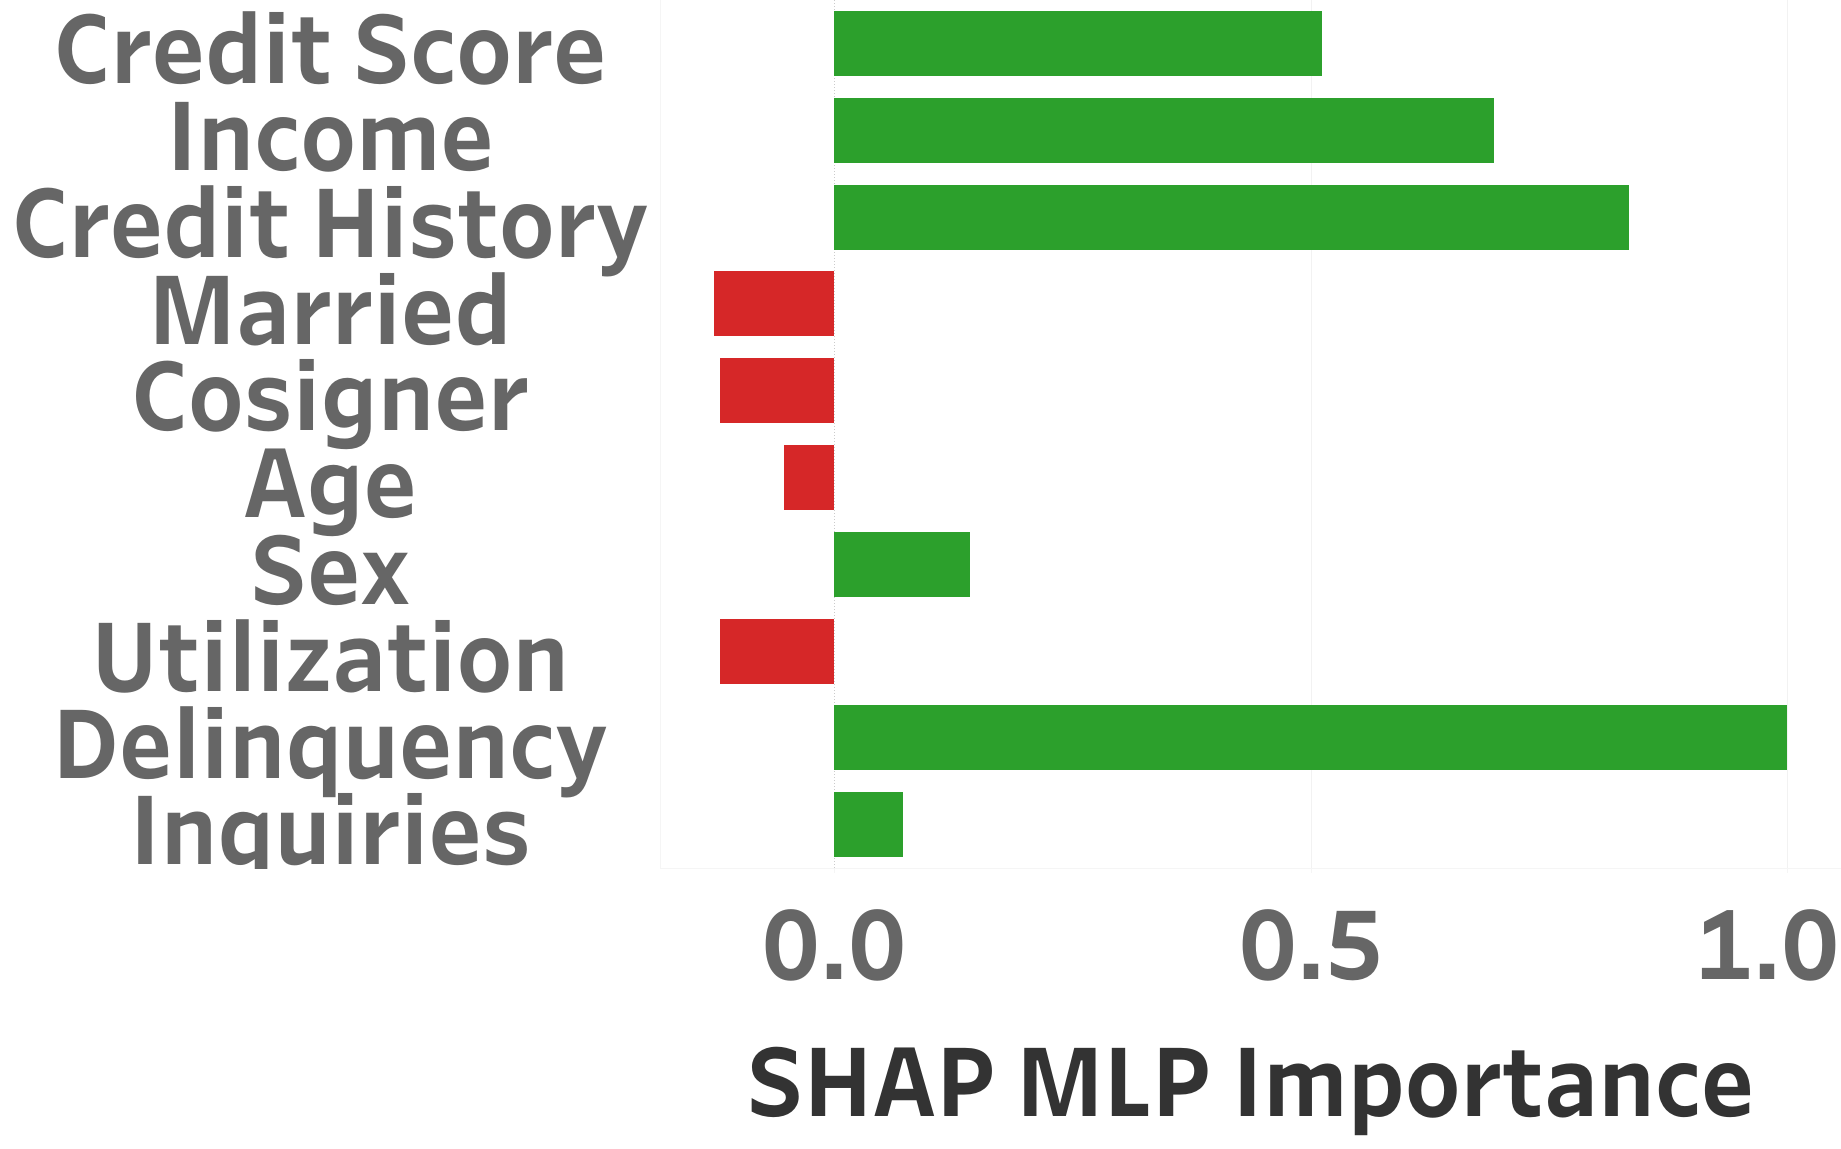
\includegraphics[width=\linewidth]{Figs/shap_mlp_ex.png}
    \end{minipage}}  %& \multicolumn{3}{c}{\begin{minipage}{.3\textwidth}
     % 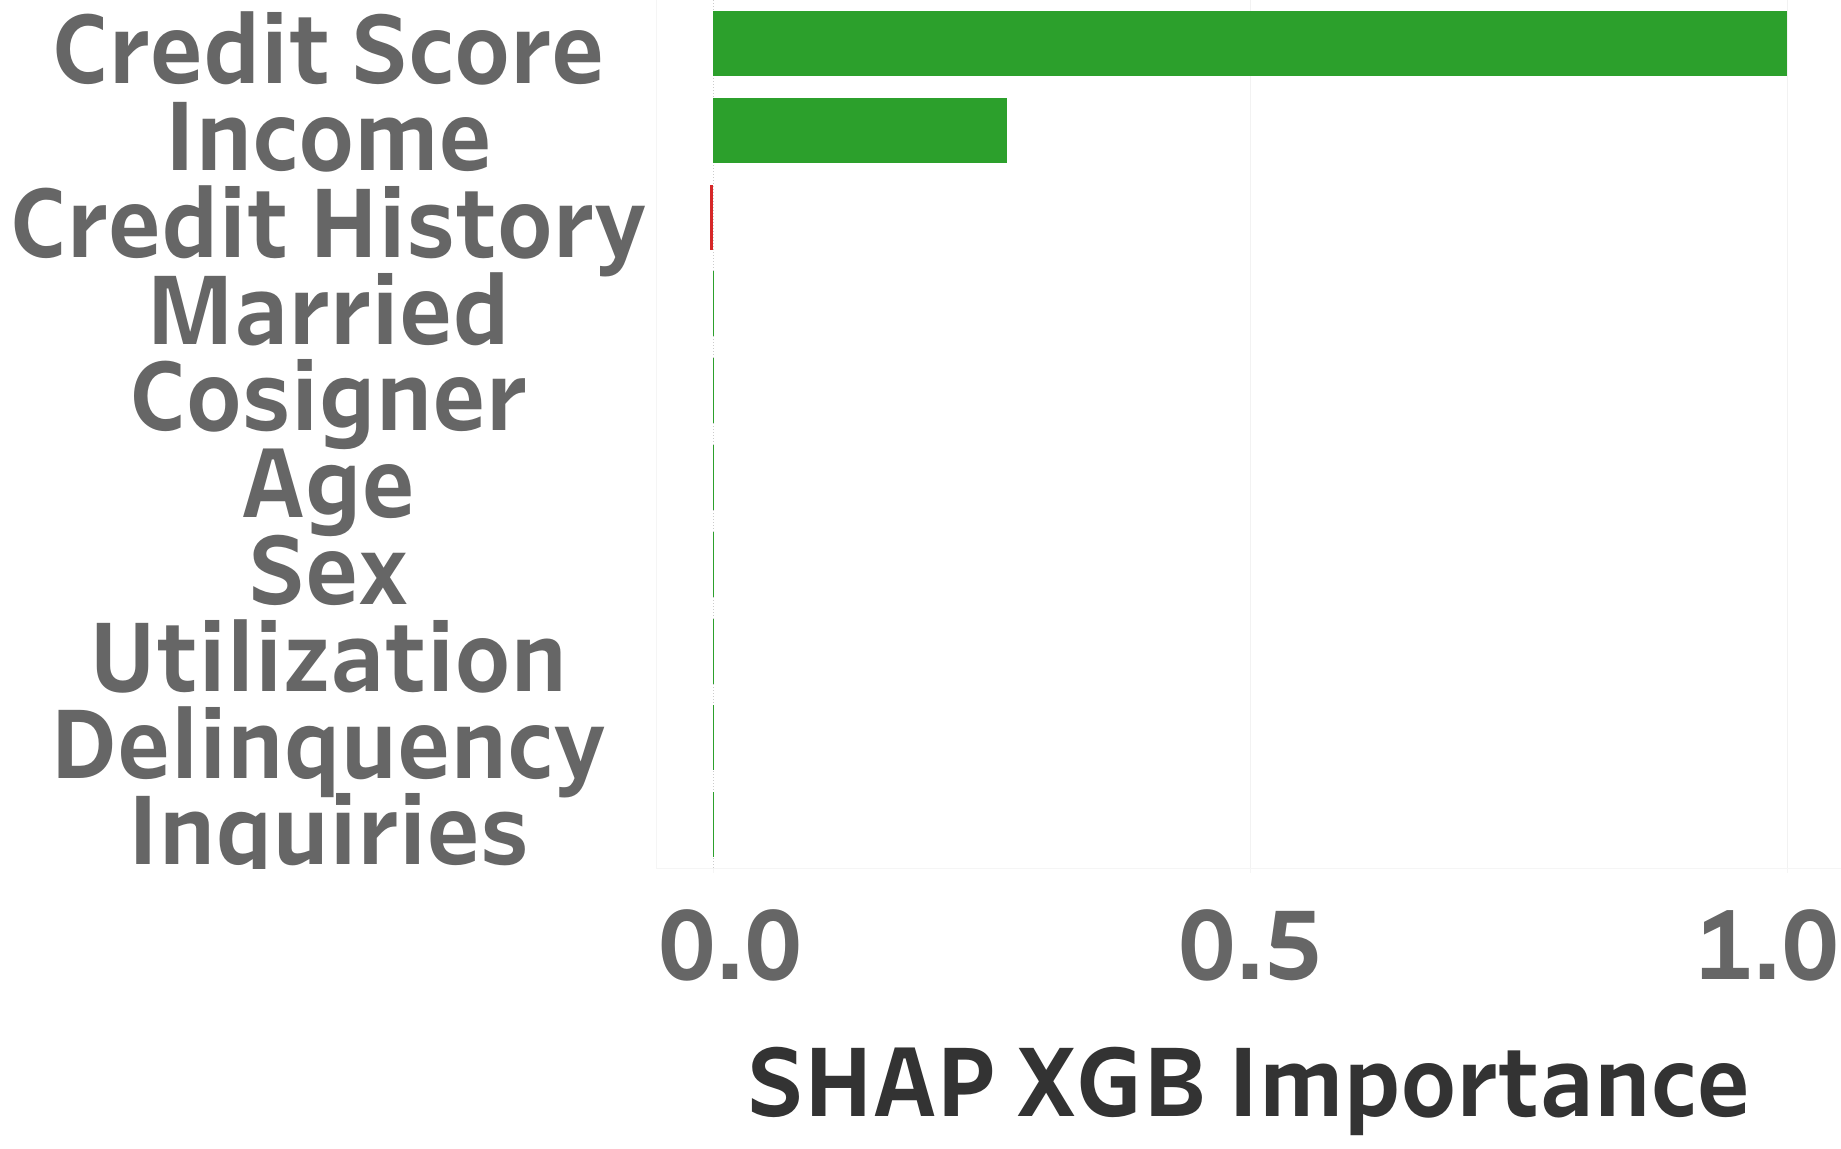
\includegraphics[width=\linewidth]{Figs/shap_xgb_ex.png}
    %\end{minipage}} 
    \tabularnewline \midrule
\end{tcolorbox}
% \noindent\begin{minipage}{\textwidth}
% \captionof{figure}{Ground truth feature importance along with qualitatively different explanations for John obtained by SHAP. %In the second pipeline, SHAP is used to explain an XGBoost model with similar performance. Feature importances are illustrated using diverging bar charts.
% }\label{box}
% \end{minipage}
\vspace{-4mm}
              \caption{Ground truth and SHAP explanation for John}
              \label{box}
            \end{subfigure}
        \caption{John's demographics along with a plot of the SHAP values obtained by explaining $\mathcal{M}$'s prediction for John.  The numbers in (b) correspond to the SHAP coefficients $e_{\text{SHAP}}(x_j)$. The red bars represent negative contributions of $e_{\text{SHAP}}(x_j)$.}
        \label{fig:shap_ex_full}
        \end{figure}


 Following how post hoc explanations are interpreted in the literature, we now inspect the $e_\text{SHAP}(x_j)$ coefficients to try to infer some information about the marginal effect of each feature. First, we can use the sign of the coefficients to infer the directionality of the impact of features. For example, we may deduce that the negative SHAP coefficient of ``Married'' in Figure \ref{box} implies that if an applicant is married, the likelihood of loan approval decreases. We could use this proposition to infer that being married has a negative relationship with loan approval in reality. Second, we can use SHAP coefficients to make inferences about the relative importance of features. For example, ``Delinquency" has the largest positive impact, while ``Married" has the largest negative impact. Finally, we can use the magnitudes of the features to identify the most influential features. In this case, ``Delinquency," ``Credit History" and ``Income" are the three most important features. 

We inspect the quality of the SHAP explanations by comparing the $e_\text{SHAP}(x_j)$ with the $\beta_j$ because the $\beta_j$ govern the ground truth relationship between explanatory variables and the target variable. Feature importance according to $\mathcal{G}$ and SHAP are shown in the left and right plots (Pipeline: $\mM=$NN) in Figure \ref{box} respectively. Unfortunately, the SHAP explanation differs significantly from the true marginal effects in every way, not just in value, but even in sign and relative importance. For example, the most important feature (largest $\beta_j$) should be ``Credit Score'' but SHAP suggests ``Delinquency'' is the most important. In addition, being married should have a positive impact on getting a loan application approved, and yet SHAP implies that the impact is negative. This example underscores the inherent pitfalls in relying on post hoc explanations to deduce the true marginal effects in the data, offering a stark illustration of how their application can yield misleading interpretations. 

%Beyond the evident misalignment, the inconsistency of the explanations further compounds the problem. Repeating the pipeline with alternative selections for $\mathcal{M}$ while maintaining all other parameters constant yields divergent SHAP explanations, as shown in the right plot of Figure \ref{fig:shap_ex}. These explanations vary greatly; the only point of agreement is that ``Credit Score" and ``Income" are important features assigned positive Shapley values. 
The demonstration of the \textit{misalignment} %and \textit{inconsistency} 
of post hoc explainers in Figure \ref{box} above motivates the main thrust of this paper. That is, we want to find out why post hoc explainers are misaligned, what resulting harm could be done to researchers using such explainers, and what mitigation strategies could be employed for recourse. 
The ensuing sections will explicate the risks associated with employing post hoc explanations to make inferences about marginal effects. We aim to provide a detailed theoretical foundation for their limitations and a thorough critique backed by empirical evidence, revealing the dangers of this approach.
%   We see from the difference in relative magnitudes of the coefficients from $e(x_j)$ in Figure \ref{fig:shap_ex} and the ground truth in Equation \ref{eqn:gt} that the explanation for John's approval is unfaithful.


%\subsection{Inconsistency Across Pipelines}
    % We simulate this scenario and show the results obtained by the two researchers in \ref{box}. We also compare the LIME explanations they receive with the ground truth. The plots at the bottom left, bottom middle, and bottom right show the importance of each feature. The features are vertically ordered from most to least important to $\mathcal{G}$. Feature importance values for the NN and XGBoost models come from LIME's explanation of the models' decisions to approve John. They are max-normalized. The feature importance values for the ground truth are represented as the max-normalized coefficients of $\mathcal{G}$ from Equation \ref{eqn:gt}. We use max-normalization because the feature importance values of LIME and the coefficients of $\mathcal{G}$ occur on different scales. In the left and middle panels, the feature importance plots being visualized are for the ground truth and NN from the previous section. For the right panel, we trained an XGBoost model with 3 estimators that achieves about an $85\%$ test set accuracy. Although they had similar accuracies, the NN and XGBoost models may have captured different correlations in the data because the explanations of the NN and XGBoost models were quite different from each other. The explanations of both black boxes were unfaithful and both had distinct errors (otherwise all three feature importance plots would look nearly identical). To see this, note that in pipeline 1 credit inquiries are implied to be the most important even though credit score is actually the most important. Also note that although credit score was correctly identified as the most important in pipeline 2, all the other features, except income, were incorrectly implied to be negligible. The explanations of pipelines 1 and 2 are also contradictory in that in pipeline 1 being male (sex$=1$) has a positive impact on approval chances while in pipeline 2 being male has a negative impact. 
     





\section{Misalignment of Post Hoc Explanations}
\label{sec:misalignment}
  In this section, we study the research problem in more depth. We first describe how we evaluate explanations in Section \ref{sec:evaluating_faithfulness}. 
  Then, in Section \ref{sec:causes_of_misalignment}, we identify properties of the data $\mD$, the model $\mM$, and the explainer $\mE$ used in a pipeline that lead to misaligned explanations and demonstrate how those individually affect the explanation. Finally, we adduce the generality of the problem of misalignment in Section \ref{sec:pervasive}. %%The experiments in this section all use our running example of explaining loan application decisions, where the ground truth model is a linear model. 

\subsection{New Metrics for Assessing Post hoc Explanations}
   \label{sec:evaluating_faithfulness}
  Both SHAP and LIME provide a feature importance measurement for each feature $j$, which we denote by $e_\mE(x^{(i)}_j)$, where $\mE$ represents the explainer.
   Our goal is to investigate whether $e_\mE(x^{(i)}_j)$ can be used to provide correct information about the marginal effect of feature $j$. To this end, we propose three new metrics that capture different aspects of explanations, each motivated by practical use cases of explanations from the literature: sign, importance ranking, and relevance. 
     
     First, we give a more detailed definition of the true marginal effects $\boldsymbol{\beta}$ so that our estimand is clear. Our characterization of $\boldsymbol{\beta}$ captures both the correlative effect that each explanatory variable has on the response variable individually as well as any effects that one variable can have on the target through other variables that depend on it. This is accomplished by considering two cases in our definition. If a feature $X_j$ does not depend on any other feature, we define $\beta_j$ to be the total derivative $\dv{Y}{X_j}$. Otherwise, we define $\beta_j = \pdv{Y}{X_j}$. Therefore, for linear models, the marginal effects equal the model coefficients.



         
         % The metrics we propose are motivated by how the post hoc feature importances are used in business research.
          We design three metrics to evaluate data-alignment  considering the practical use case of the explanations. Researchers using SHAP and LIME typically use the feature importance values in three main ways: 1) inspect the sign of the feature importance values to identify how the features impact the outcome they are interested in %For example, in \citep{park2024extracting} says that the quad-core feature of smartphones having a negative SHAP value also indicates a negative effect on consumer choices. 
         2)  identify the relative importance of features %This type of analysis is exemplified in \citep{zhang2023explainable}, which advocates for managers to use the top most important features from the ranking they obtained via SHAP as early indicators of financial risk in manufacturing companies. 
         and 3) identify the most influential features. %cite kovvuri
    %To capture how well SHAP and LIME can do these things, we use three metrics. 

    The first metric, termed \textbf{directionality}, measures whether post hoc explainers can at least identify the correct \textit{sign} of a feature's influence on the outcome. It evaluates an explanation only qualitatively. We calculate directionality by determining the percentage of instances where the sign of $e_\mE(x^{(i)}_j)$ matches that of $\beta_j$ for each feature $j$ across $m$ instances in the test set. %However, when $\beta_j$ is sufficiently small, checking the sign agreement would be too strict. Thus, we relax the definition and instead check if $\mid e_\mE(x^{(i)}_j)\mid $ is also very small relative to the largest feature importance value $\max_{j^\prime} \mid e_\mE(x^{(i)}_{j^\prime}) \mid $.
    % Given the ground truth $\beta_j$ and feature importance values $e_\mE(x^{(i)}_j)$ from an explainer, we denote the accuracy for the $j^{\text{th}}$ feature as follows. 
    % Note that this definition is  made in reference to the entire test set $\{x^{(i)}\}_{i=1}^n$ but considers only one feature index $j$.  %The notation $\hat{\beta}^{(i)}$ represents a feature importance vector for the $i^{\text{th}}$ test set instance. 
    \begin{equation}
        \label{eq:acc}
        \texttt{directionality}(\{e_\mE(x^{(i)}_j)\}_{i=1}^m,\beta_j) = \frac{1}{m} \sum_{i=1}^m s_j( e_\mE(x^{(i)}_j),\beta_j)
    \end{equation}
    where 
    \begin{equation*}
        s_j(e_\mE(x^{(i)}_j),\beta_j) = \begin{cases*}
                    \mathbf{1}_{\mathbb{R}^+}(\beta_j \cdot e_\mE(x^{(i)}_j)) & if  $\mid \beta_j\mid > \epsilon_1$  \\
                     \mathbf{1}_{(0,\epsilon_2)}\left(\frac{\mid e_\mE(x^{(i)}_j)\mid }{\max_{j'} \mid e_\mE(x^{(i)}_{j'})\mid}\right) & otherwise
                 \end{cases*}
    \end{equation*}
    Here $\mathbf{1}_S(z)$ is an indicator function that returns 1 if $z\in S$ and outputs 0 otherwise. $s_j(e_\mE(x^{(i)}_j),\beta_j)$ is designed to facilitate a relaxed version of accuracy by checking if $\beta_j$ and $e_\mE(x^{(i)}_j)$ have the same sign only when $\beta_j$ is not very small, i.e., larger than $\epsilon_1$. When $\beta_j$ is small, $s_j$ instead checks if $e_\mE(x^{(i)}_j)$ is small relative to the other $e_\mE(x^{(i)}_{j^{\prime}})$, where $j^\prime \neq j$. In particular, the ratio of $\mid e_\mE(x^{(i)}_j)\mid $ and $\max_j^\prime \mid e_\mE(x^{(i)}_{j^\prime})\mid$ should be small. We check this using a variable threshold $\epsilon_2$. In our experiments, we use $\epsilon_1=1e-2$ and $\epsilon_2=1e-2$. This definition uses a relaxed conception of accuracy because, for example, if the ground truth value is 0.001 and the explanation returns -0.001, we would consider it correct, even if the signs do not agree, because both suggest that the feature has a very small impact on $Y$.
    
      The second metric, \textbf{concordance}, measures how accurately the explanations recover the \textit{relative importance} of features compared to the ground truth ranking induced by $\boldsymbol{\beta}$. Given the $e_\mathcal{E}(x^{(i)}_j)$, we rank the features from least to most important and calculate the \emph{Spearman Rank Correlation} \cite{spearman1904proof} between this ranking and a ranking of the $\beta_j$. While the directionality metric is computed using the entire test set per feature, the concordance is computed per instance using all features.

    % The Spearman rank correlation is defined as follows. 
    \begin{equation}
       \texttt{concordance}(e_\mE(\mathbf{x}^{(i)}),\boldsymbol{\beta}) = 1 - \frac{6\sum_{j=1}^d (\text{rank}(\beta_j) - \text{rank}(e_\mE(x^{(i)}_j)))^2}{d(d^2-1)},
    \end{equation}
    Above, $d$ is the number of features and $\text{rank}(\beta_j)$ and $\text{rank}(e_\mE(x^{(i)}_j))$ denote the rank of the $j^{\text{th}}$ feature according to the coefficients of $\boldsymbol{\beta}$ and explanations $e_\mE(\mathbf{x}^{(i)})$, respectively. If an explainer's rankings are 100\% correct, then this correlation should be 1. Any value less than 1 indicates an error in the rankings (which can lead users to misinterpret the importance of some features).
    
Third, motivated by the fact that researchers may only be interested in identifying a small set of features that have the highest impact, we define the third metric, \textbf{relevance}, based on the ranking of features. Our metric, denoted $\text{relevance}_k$, measures how many of the top $k$ most important features according to $\mathcal{E}$  are among the top $k$ largest (in magnitude) marginal effects. Denote by $I_k^+(e_\mE(\mathbf{x}^{(i)}))$ and $I_k^+(\boldsymbol{\beta})$  the set of feature indices among the top $k$ most highly ranked according to $e_\mE(\mathbf{x}^{(i)})$ and $\boldsymbol{\beta}$, respectively. Then we define 
    \begin{equation}
        \texttt{relevance}_k(e_\mE(\mathbf{x}^{(i)}), \boldsymbol{\beta}) = \frac{\mid I_k^+(\boldsymbol{\beta}) \cap I_k^+(e_\mE(\mathbf{x}^{(i)}))\mid}{k}.
    \end{equation}
     Like the concordance metric, $\text{relevance}_k$ is also computed at the instance level. 
    In our experiments, we compute $\text{relevance}_k$ for each $k$ and plot the means and standard errors over $m$ instances. $\text{relevance}_k(e_\mE(\mathbf{x}^{(i)}), \boldsymbol{\beta})$ represents the recall for the identification of features among the top-$k$ largest marginal effects according to $\mathcal{E}$.       
    
   
        



                    \begin{figure}[ht!]
            \centering
            \begin{subfigure}[t]{.28\textwidth}
              \centering
              \captionsetup{justification=centering}
                  \raisebox{.2cm}{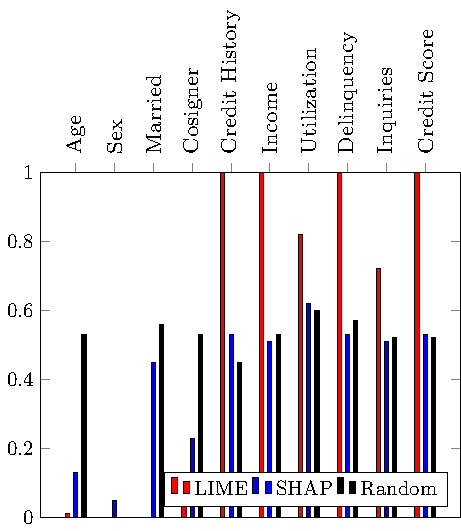
\includegraphics[width=\textwidth]{Figures/sec4_1-figure0.pdf}}%{Figures/lime_shap_Spearman_magnitude.png}

              \caption{Directionality}%Spearman rank correlations of feature importance magnitudes from SHAP and LIME against the true ranking from $\mathcal{G}$. }
               \label{fig:lime_shap_sign_accs}
            \end{subfigure}%
            \hspace{1cm}%\hfill
            \begin{subfigure}[t]{.28\textwidth}
              \centering
               \captionsetup{justification=centering}
              \raisebox{.05cm}{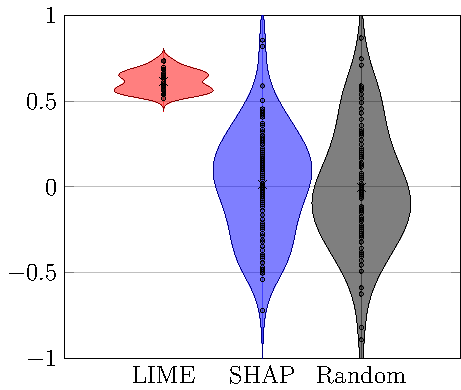
\includegraphics[width=\textwidth]{Figures/sec4_1-figure1.pdf}}%{Figures/lime_shap_Spearman_signed.png}
              \caption{Concordance}%Spearman rank correlations of signed feature importance from SHAP and LIME against the true ranking from $\mathcal{G}$.}
               \label{fig:lime_shap_Spearman_signed}
            \end{subfigure}
            \hspace{1cm}%\hfill
            \begin{subfigure}[t]{.28\textwidth}
              \centering
               \captionsetup{justification=centering}
            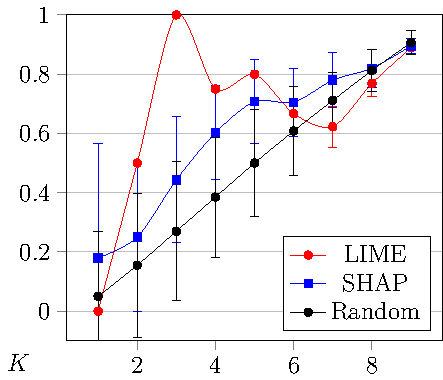
\includegraphics[width=\textwidth]{Figures/sec4_1-figure2.pdf}%
            \caption{Relevance}%The average and standard error of recall of SHAP and LIME when attempting to capture the top K most important features to $\mathcal{G}$ when explaining $\mathcal{M}$, for varied $K=1,2,3,...$ number of features.}
            \label{fig:avg_recall}
            \end{subfigure}
            \caption{The data alignment evaluation in three aspects. For plot (c) each point in the line plot represents a mean relevance for a given $k$. The error bars represent the standard error. The total number of features is 10.}
           \label{fig:beta_alignment}
        \end{figure}    
 
  We call the evaluation of the directionality, concordance, and relevance the evaluation of \textbf{data-alignment}. We evaluate the data-alignment
 for SHAP and LIME on $m=100$ applicants randomly selected from the test set and report the results in Figure \ref{fig:beta_alignment}. 
 We find that neither SHAP nor LIME achieves satisfying results on any of the three dimensions. Most notably, in spite of the fact that SHAP is strongly favored over LIME by researchers (91\% vs 14\% from the papers we surveyed), SHAP performs significantly worse than LIME in all three dimensions. SHAP cannot even identify the correct directionality of the features, let alone the concordance. To have a better understanding of SHAP, we also simulate a \emph{random} explainer that randomly draws its feature importance values $e_\text{random}(x^{(i)}_j)$ from a standard normal distribution for each $j$ and $i$. We find that \emph{SHAP explanations do not have better data-alignment than random explanations  with respect to directionality and concordance.}         


\subsection{Pervasiveness of Data-Misalignment - a Large Scale Evaluation}
    \label{sec:pervasive}
    So far, we have only used one simulated dataset to demonstrate the misalignment of SHAP and LIME explanations. To study how pervasive the issue is, % We show that data-misalignment is a general property of SHAP and LIME. In doing this, the implications of Section \ref{sec:causes_of_misalignment} are corroborated and the scope of their validity is widened. We do this by evaluating the data-alignment of 
    we evaluate the SHAP and LIME explanations using 100 simulated datasets.
    
    Our 100 synthetic datasets have randomly selected numbers of features between 3 and 100, and randomly selected numbers of rows between 100 and 10000. The features are i.i.d. according to $\mathcal{N}(0,5)$. The target of each dataset is binary and is produced using randomly generated linear decision boundaries. To generate the linear decision boundaries, we randomly generated integer coefficients between -10 and 10 and used SymPy to construct the linear decision functions with those coefficients. Each dataset used one of these functions to generate labels for each sample.  %We vary the amount of label noise in each dataset by fixing a probability $p \in [0,.1]$ before generating the dataset and then flipping each label with probability $p$.
    We split each dataset into 80\% training data and 20\% testing data.  The test set accuracies of all models fall between $.82$ and $.99$. It is important to note that as these datasets all have i.i.d. normal features and there is no noise in the target column, this experiment uses practically ideal conditions for the training and subsequent explanation of ML models.


        Since the number of features differs across the datasets, we report the results for our three metrics in the following fashion, conditioned on the number of features. %For directionality, for each $d$, we report the mean directionality for the actual most important feature over 100 test set instances from the datasets with dimension $d$. 
        For each dataset, we compute feature-wise mean directionality, mean concordance over $m$ test instances, and mean relevance for $k=3$ over $m$ test instances. This gives us a single measurement of each metric for each dataset. We partition the results for each dataset based on which of the ten equal width bins of [0,100] the associated $d$ falls into. Finally, we report the means within each bin for each metric.  %We report the information similarly for the number of rows $n$ rather than $d$ below.   

    
    Our experimental results imply that SHAP and LIME explanations are generally not informative about marginal effects for datasets with more than thirty features. Indeed, Figure \ref{fig:lime_shap_vary_d} shows that, generally when $d$ exceeds $30$, mean directionality for SHAP and LIME is actually under $.5$ which is worse than random guessing. This is an alarming sign because the two most popular post hoc explainers can not even get the correct qualitative estimation of the true marginal effect --- even the sign is wrong! In addition, both the mean concordance and mean relevance for $k=3$ are near $0$. It should be noted that the more features there are, the more challenging it is for the two explainers to correctly identify the contributions of each feature, as there exist more possible mappings from the input to the output that could be different from that of $\mG$ and there is no control over which one $\mM$ uses. In general, we noticed a negative association between $d$ and each of our metrics. We did not notice significant associations between $n$ and our metrics.

      \begin{figure}[ht!]
      \captionsetup{labelfont=footnotesize,textfont=footnotesize}
      \captionsetup[subfloat]{labelfont=scriptsize,textfont=scriptsize,justification=centering}
      \centering
      \subfloat[SHAP Mean Directionality]{%
        \hspace{0mm}
        \raisebox{0cm}{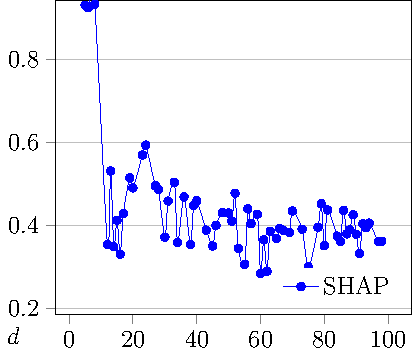
\includegraphics[width=0.178125\textwidth]{SynthFigs/meanaccshap-figure0.pdf}\quad}%
        \label{fig:shap_vary_d_spearmans}%
      }\hspace{1cm}%\hfill
      \subfloat[SHAP Concordance]{%
        \raisebox{0cm}{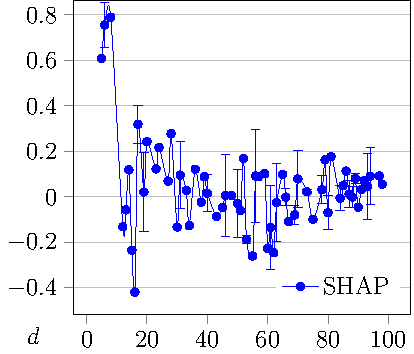
\includegraphics[width=0.178125\textwidth]{SynthFigs/concshap-figure0.pdf}}%
        \label{fig:shap_vary_d_accs}%
      }\hspace{1cm}%\hfill
      \subfloat[SHAP Top-3 Relevance]{%
        \raisebox{0cm}{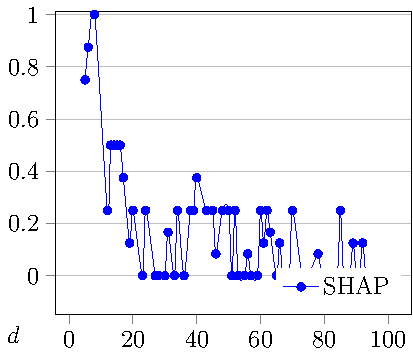
\includegraphics[width=0.178125\textwidth]{SynthFigs/relshap-figure0.pdf}}%
        \label{fig:shap_vary_d_spearmans}%
      }\\
      % \subfloat[LIME Top-1 Directionality]{%
      %   \raisebox{0cm}{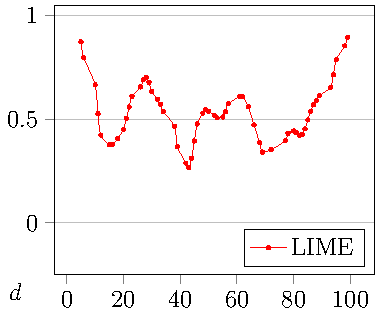
\includegraphics[width=.2\textwidth]{Figs/synthetic-figure1.pdf}}%
      %   \label{fig:lime_vary_d_accs}%
      % }\hspace{.5cm}%\hfill
      \subfloat[LIME Mean Directionality]{%
        \hspace{0mm}
        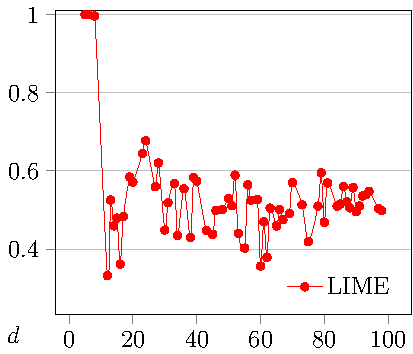
\includegraphics[width=0.178125\textwidth]{SynthFigs/meanacclime-figure0.pdf}\quad%
        \label{fig:lime_vary_d_spearmans}%
      }\hspace{1cm}%\hfill
      \subfloat[LIME Concordance]{%
        \hspace{0mm}
        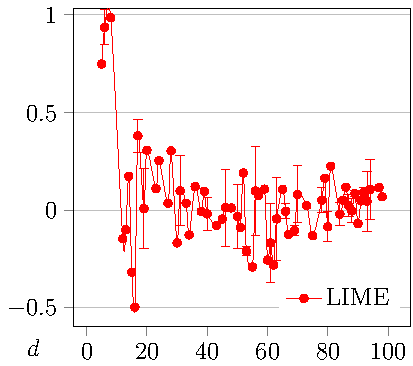
\includegraphics[width=0.178125\textwidth]{SynthFigs/conclime-figure0.pdf}%
        \label{fig:lime_vary_d_accs}%
      }\hspace{1cm}%\hfill
      \subfloat[LIME Top-3 Relevance]{%
        \hspace{0mm}
        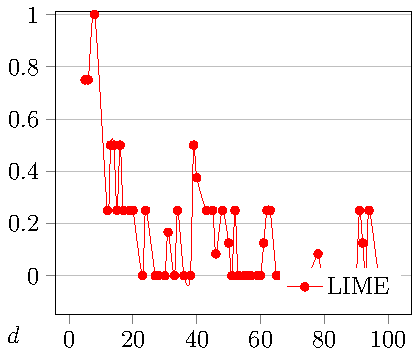
\includegraphics[width=0.178125\textwidth]{SynthFigs/rellime-figure0.pdf}%
        \label{fig:lime_vary_d_spearmans}%
      }\\
      \caption{Relationship of number of features $d$ with feature-wise mean directionality, concordance, and relevance for $k=3$}
      \label{fig:lime_shap_vary_d}
    \end{figure}




  
    \subsection{Contributing Factors to  Misalignment}
        \label{sec:causes_of_misalignment}
        We investigate factors in the pipeline that contribute to misalignment in terms of sign, relative importance, and relevance compared to the ground truth marginal effects, as aforementioned. Our aim is to provide both theoretical and empirical evidence for why post hoc explanations should not be used to make inferences about the actual input-output relationships underlying data. Our investigation will examine both stages of the explanation pipeline (the prediction stage and the explanation stage). % We first investigate SHAP and LIME in the explanation stage to show how their inherent model design contributes to misalignment. 
        We work under the assumptions that domain knowledge about the data generation process is unavailable. Due to space limitations, we show the experiment on one dataset, but all experiments are repeated on a different dataset in the Appendix. %The experiments in this section involve first training an ML model $\mathcal{M}$ and then building an explainer model $\mathcal{E}$ to produce explanations. % training data to build a machine learning model and then and explanations of predictions of those NNs on instances from the remaining 20\% of data reserved as a test set.


    \subsubsection{Explainers May Inherently Be Misaligned}
    \label{sec:theoretical_considerations}
   We first investigate how the explainers themselves contribute to misalignment by deriving and analyzing equations for their explanations of linear models. To exclude other factors in the explanation pipeline, we assume here that we have access to the ground truth model $\mathcal{G}$ and that SHAP and LIME are directly applied to explaining $\mathcal{G}$ rather than $\mathcal{M}$. Thus, the explanations are solely based on the explanation stage. We suppose that $\mathcal{G}$ is a linear function of $d$ features and SHAP and LIME explain the output of $\mathcal{G}$ at a point $\boldsymbol{\xi}$, that is, $\mathcal{G} = \boldsymbol{\beta}^T \mathbf{x}$ where $\mathbf{x} \sim \mathcal{N}(\mathbf{0},\mathds{1}_d)$ and $\boldsymbol{\xi}$ is a realization of $\mathbf{x}$. Below, we derive mathematical representations of SHAP and LIME explanations, and investigate their relationships with the marginal effects $\boldsymbol{\beta}$.

         \paragraph{$e_{\text{SHAP}}$ when Explaining a Linear Model}
              %SHAP does \emph{not} recover $\boldsymbol{\beta}$ and should not be relied upon for this purpose. 
              The importance of the $j^{th}$ feature of the $i^{th}$ data sample $\xi^{(i)}_j$ in a SHAP explanation is the Shapley value for that feature in that sample. The Shapley value reduces to the following expression when SHAP is used to explain a linear model according to \cite{StrumbeljErik2014Epma,lundberg17shap}. 
             \begin{equation}
                \label{eqn:shap_gt}
                e_\text{SHAP}(\mathbf{x}^{(i)}_j) = \beta_j (\xi^{(i)}_j - \bar{x}_j).
             \end{equation}

            
The SHAP explanations outlined by Equation \ref{eqn:shap_gt} exhibit several undesirable properties that can limit their practical application. For instance, when $\boldsymbol{\xi}=\bar{\mathbf{x}}$, the SHAP values $e_\text{SHAP}$ reduce to 0, leading to all features being deemed unimportant. Moreover, Shapley values cannot be used to infer the signs of the marginal effects because when $\xi^{(i)}_j - \bar{x}_j$ is negative, the signs of $e_{\text{SHAP}}(\xi^{(i)}_j)$ and $\beta_j$ are opposite. Another consequence of Equation \ref{eqn:shap_gt}  is that the expected SHAP values average to zero, rendering them generally uninformative about the marginal effects. Some authors address this in their search for global feature importance by instead considering empirical averages of absolute SHAP values \citep{lenaers23rent,maeng23vr,guenther2023useful}. However, this obviously comes at the cost of losing information about the directionality of a feature's impact.

             Following Equation \ref{eqn:shap_gt}, we propose to mitigate SHAP's inherent misalignment for linear models by using what we will refer to as \emph{normalized SHAP values}: $e_{\text{SHAP}}(\xi^{(i)}_j) / (x^{(i)}_j - \bar{x}_j)$. Although this is a straightforward adjustment that can be made in order to approximate the marginal effects using SHAP, we are not aware of its use in prior literature.  Our empirical evaluation of these normalized Shapley values, which includes recalculating directionality, concordance, and comparison with traditional SHAP results (illustrated in Figures \ref{fig:shap_dividex_corr}), suggests significant improvements. Normalized SHAP values frequently exhibit correct sign alignment and generate feature rankings more concordant with ground truth. Directionality for features related to credit score improved remarkably, as shown in Figure \ref{fig:shap_dividex_accs}. However, directionality for the features related to cosigner access (``Married" and ``Cosigner") decreased. The improvements to feature rankings are evident from Figures \ref{fig:shap_dividex_spearmans} and \ref{fig:shap_dividex_recalls}; we can see that mean concordance rose from near 0 to about .6 and relevance was improved substantially for $k=2,3,4,5$. 
             
            
             Given the evident effectiveness of the SHAP normalization scheme and our evidence that unmodified SHAP explanations are theoretically  data-misaligned, \textbf{we will adopt this normalization approach for all subsequent experiments in this paper}. This is vital as we explore the impacts of $\mathcal{M}$'s predictive performance and feature independence in subsequent sections (\ref{sec:role_of_predictive_power} and \ref{sec:role_of_correlation}). %For example, we will use it in the following subsections on the roles of $\mathcal{M}$'s predictive performance and feature independence (\ref{sec:role_of_predictive_power} and \ref{sec:role_of_correlation}). We wish to show that increasing the predictive performance of $\mathcal{M}$ and using independent training data features may increase data-alignment, so the normalization scheme is necessary because otherwise SHAP's explanations are similar to random ones and thus will be unaffected by external effects. 
           \begin{figure}[ht!]
            \centering
            \begin{subfigure}[t]{.28\textwidth}
              \centering
              \captionsetup{justification=centering}
                  \raisebox{.2cm}{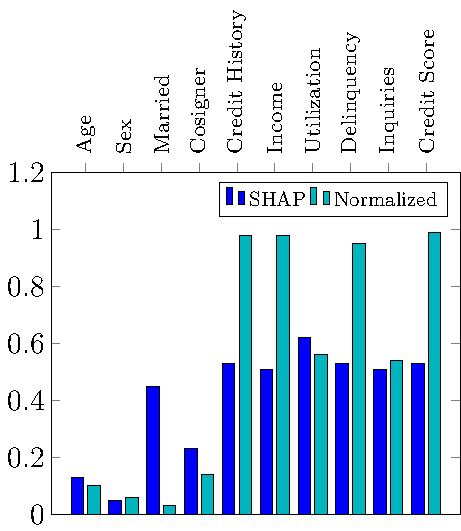
\includegraphics[width=\textwidth]{Figures/sec4_1_dividex-figure0.pdf}}%{Figures/lime_shap_Spearman_magnitude.png}

              \caption{Directionality}%Spearman rank correlations of feature importance magnitudes from SHAP and LIME against the true ranking from $\mathcal{G}$. }
               \label{fig:shap_dividex_accs}
            \end{subfigure}%
            \hspace{1cm}%\hfill
            \begin{subfigure}[t]{.28\textwidth}
              \centering
               \captionsetup{justification=centering}
              \raisebox{.05cm}{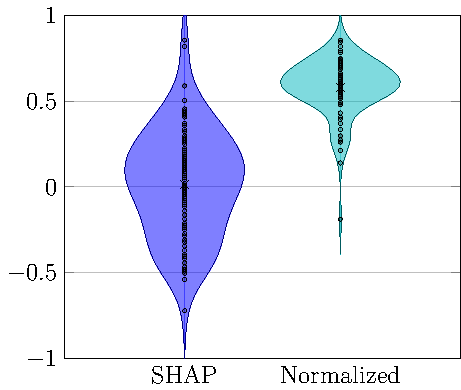
\includegraphics[width=\textwidth]{Figures/sec4_1_dividex-figure1.pdf}}%{Figures/lime_shap_Spearman_signed.png}
              \caption{Concordance}%Spearman rank correlations of signed feature importance from SHAP and LIME against the true ranking from $\mathcal{G}$.}
               \label{fig:shap_dividex_spearmans}
            \end{subfigure}
            \hspace{1cm}%\hfill
            \begin{subfigure}[t]{.28\textwidth}
              \centering
               \captionsetup{justification=centering}
            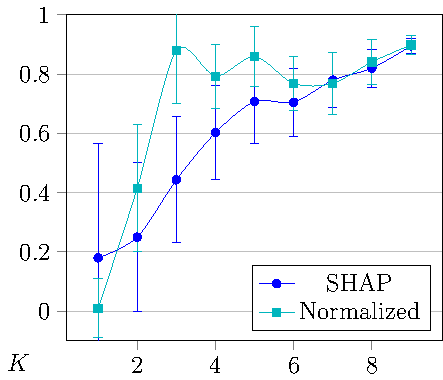
\includegraphics[width=\textwidth]{Figures/sec4_1_dividex-figure2.pdf}%
            \caption{Relevance}%The average and standard error of recall of SHAP and LIME when attempting to capture the top K most important features to $\mathcal{G}$ when explaining $\mathcal{M}$, for varied $K=1,2,3,...$ number of features.}
            \label{fig:shap_dividex_recalls}
            \end{subfigure}
            \caption{Comparison of SHAP explanations without and with SHAP value normalization}
           \label{fig:shap_dividex_corr}
        \end{figure}   
        \paragraph{$e_{\text{LIME}}$ when Explaining a Linear Model}
            \label{sec:lime_linear_case}
             %In this section we we will show that there are conditions when the LIME coefficients have the property $e(x_j)\simeq \beta$ and use this fact to justify that  $e(x_j)$ can be evaluated with respect to the ground truth $\boldsymbol{\beta}$. Those conditions are discussed in the next paragraph. 
             LIME works by sampling data points around a given instance, then using these samples to train a weighted linear model as a local surrogate model that approximates the predictions of the original complex model in the vicinity of the instance. The local surrogate model is trained as a weighted ridge regressor. To obtain interpretable and sparse explanations, LIME discretizes numerical features and includes a regularization component to promote sparsity in the local surrogate models it creates. This regularization helps in selecting a subset of features that are most influential for predictions near the instance being explained, thus ensuring that the explanations are both interpretable and concise. However, the above aspects of LIME's design may compromise its ability to accurately recover the true marginal effect coefficients. 
             
             The use of discretized features in LIME's ridge regression model can eliminate critical information about the  model being explained. Additionally, the sparsity penalty which is used in ridge regression may zero out coefficients for features that actually have a non-zero marginal effect, distorting the picture one may obtain of the marginal effects. Moreover, employing weighted ridge regression introduces a weight matrix that further skews the estimation of marginal effects. This distortion can be observed in the closed-form solution of the weighted ridge regression, indicating potential limitations in LIME's ability to provide accurate estimates under certain conditions.
             
              Having identified the aforementioned properties of LIME's regression design as contributors to its lack of data-alignment, we derive conditions under which LIME would be data-aligned. We begin this effort by deriving the following closed form for the expected LIME coefficients in an idealized scenario where LIME does not use discretization and the model being explained is a linear function of i.i.d. normal features. The scenario and form of the coefficients are given in Theorem \ref{thm:lime_thm} below. Our Corollary 1 analyzes the closed form for the coefficients in order to ascertain the conditions for LIME's alignment in this idealized scenario. 
            \begin{theorem}
                \label{thm:lime_thm}
                Suppose $f:\mathbb{R}^d\rightarrow \mathbb{R}$ that maps $\mathbf{x} \mapsto \boldsymbol{\beta}^T \mathbf{x}$, is explained at a sample $\boldsymbol{\xi}$ drawn from $\mathcal{N}(\mathbf{0}, \mathds{1}_d)$ with LIME. LIME uses a generalized ridge regressor as a surrogate model with sparsity penalty parameter $\lambda=1$ and shrinkage target equal to the identity matrix $\mathds{1}_d$. Suppose further that LIME  does not discretize features, samples i.i.d. data points $\mathbf{x}^{(1)},\ldots,\mathbf{x}^{(n)}$ from $ \mathcal{N}(\boldsymbol{\xi}, \mathds{1}_d)$, and weights those samples with the exponential kernel $\pi(\boldsymbol{\xi},\mathbf{x}) = exp(-\norm{\boldsymbol{\xi}-\mathbf{x}}_2^2/2\nu^2)$ using bandwidth $\nu>0$. %%Then, in the large $n$ limit, the coefficients of LIME converge to $\boldsymbol{\beta}$. That is, for each $\mathbf{x}^{(i)}$, $e_{\text{LIME}}(x^{(i)}_j) \rightarrow %\boldsymbol{\beta}$
                %as $n \rightarrow \infty$.
                Denote the matrix of samples $\mathbf{X}$. % and the estimated LIME coefficients using a given $\mathbf{X}$ as $\hat{\mathbf{u}}$.
                % Then, given $\eta>0$ and $\epsilon > 0$ there exists $N'$ such that for $N > N'$
                % \begin{equation}
                %     \norm{\hat{\mathbf{u}} - \mathbf{u}}
                % \end{equation}
                 Then the theoretical coefficients for LIME in expectation over the random matrices $\mathbf{X}$ are given by 
                \begin{equation}
                    \mathbf{u} = (c_1\boldsymbol{\xi} \boldsymbol{\xi}^T - c_2 \mathbf{I})(\boldsymbol{\xi}\boldsymbol{\xi}^T + c_3 \mathbf{I})\boldsymbol{\beta}
                \end{equation}
                where $c_1,c_2,c_3$ are constants depending on $\nu$, $n$, and $d$. 
            \end{theorem}

             % Although LIME does not recover $\boldsymbol{\beta}$ with its default settings, Theorem 2 shows that $e_{\text{LIME}}(\mathbf{x}^{(i)}_j)$ converges to $\boldsymbol{\beta}$ in the large $n$ limit when explaining a linear model $\boldsymbol{\beta}^T \mathbf{x}$ where the data $\mathbf{x}$ are sampled from a standard multivariate normal distribution and LIME does not discretize continuous features. 


             Theorem 1 gives a closed form for LIME coefficients $\boldsymbol{u}$ in expectation over the distribution of random samples $\mathbf{X}$. By investigating the relationship of $\boldsymbol{u}$ with $\nu$ and $n$ we can understand sufficient conditions for LIME to extract $\boldsymbol{\beta}$. Corollary 1 below shows that as $\nu$ and $n$ grow to $\infty$, $\boldsymbol{u}$ converges to $\boldsymbol{\beta}$. The practical implication of this corollary is that, when using LIME without discretization, $\nu$ and $n$ should be set to be large. Notably, \cite{garreau20theoretical} obtained the same result in the case where discretization is used. Numerical experiments justifying this claim as well as the proofs for Theorem 1 and Corollary 1 can be found in the Appendix. We also show that if $\nu$ is too small the LIME coefficients all go to $\mathbf{0}$.

            \begin{corollary}
                Under the assumptions of Theorem 1, and for a given number of features $d$, the expected LIME coefficients $\mathbf{u}$ converge to $\boldsymbol{\beta}$ as $\nu$ and $n$ tend to $ \infty$. 
            \end{corollary}
             
%             Since the number of samples $n$ cannot be made infinite in practice, we investigate for additional ways users can influence data-alignment in practice. Such were illuminated by our Theorem \ref{thm:lime_bd} which is motivated by the following ideas from regression. Using the closed form of the weighted ridge regression coefficient estimates, LIME's coefficients can be written as
%             \begin{equation*}
%                 e_{\text{LIME}}(\boldsymbol{\xi})=(\mathbf{A} + \mathbf{I})^{-1}\mathbf{A} \boldsymbol{\beta}
%             \end{equation*}
%             where $\mathbf{A} = \mathbf{X}^T \mathbf{W}\mathbf{X}$ and $\mathbf{W}$ is the weight matrix for LIME's sample data.  Hence, the condition $\norm{(\mathbf{A} + \mathbf{I})^{-1}\mathbf{A}}=1$ is necessary (although not sufficient) for $e_{\text{LIME}}(\boldsymbol{\xi}) = \boldsymbol{\beta}$. Since Theorem \ref{thm:lime_thm} showed that $e_{\text{LIME}}(\boldsymbol{\xi})\rightarrow \boldsymbol{\beta}$ and this entails that $(\mathbf{A} + \mathbf{I})^{-1}\mathbf{A}\rightarrow \mathbf{I}$, this suggests that we may check how close $\norm{(\mathbf{A} + \mathbf{I})^{-1}\mathbf{A}}$ is to 1 as a proxy for $e_{\text{LIME}}(\boldsymbol{\xi})$ being close to $\boldsymbol{\beta}$ (we provide empirical evidence for this in the Appendix). Theorem \ref{thm:lime_bd} gives lower and upper bounds on $\norm{(\mathbf{A} + \mathbf{I})^{-1}\mathbf{A}}$ which enables illumination of the roles of $\nu$ and $n$ on how close $e_{\text{LIME}}(\boldsymbol{\xi})$ is to $\boldsymbol{\beta}$ using this idea.  Under the assumptions of Theorem \ref{thm:lime_thm}, solutions to LIME's ridge regression problems satisfy the following bound.
            
%             \begin{theorem}
%                 \label{thm:lime_bd}
%                  Let the $n$ samples generated by LIME be collected into a data matrix $\mathbf{X}\in\mathbb{R}^{n\times d}$ and $\mathbf{W}\in\mathbb{R}^{n\times n}$ be the ridge regression weight matrix with $w_{ii} = \pi(\boldsymbol{\xi},\mathbf{x}^{(i)})$ for $i=1,\ldots,n$ and 0 elsewhere. Define the shorthand notation $\mathbf{A}:= \mathbf{X}^T \mathbf{W}\mathbf{X}$. so that the ridge regression solution is
%                 \begin{equation*}
%                     e_{\text{LIME}}(\mathbf{x}^{(i)}_j) = (\mathbf{A} + \mathbf{I})^{-1}\mathbf{A} \boldsymbol{\beta}
%                 \end{equation*}
%                 Then
%                 \begin{equation*}
%                     \frac{\sigma_{\max}(\mathbf{A})}{\sigma_{\max}(\mathbf{A}) + 1} \leq \norm{(\mathbf{A} + \mathbf{I})^{-1}\mathbf{A}} \leq \frac{\sigma_{\max}(\mathbf{A})}{\sigma_{\min}(\mathbf{A}) + 1}
%                 \end{equation*}
%                 where $\sigma_{\min}(\mathbf{A})$ and $\sigma_{\max}(\mathbf{A})$ are the smallest and largest singular values of $\mathbf{A}$, respectively. 
%             \end{theorem}
%             The lower and upper bounds on $\norm{(\mathbf{A} + \mathbf{I})^{-1}\mathbf{A}}$ given by Theorem \ref{thm:lime_bd} depend on the minimum and maximum singular values of the matrices $\mathbf{A}=\mathbf{X}^T\mathbf{W}\mathbf{X}$, which themselves depend on the kernel bandwidth $\nu$ (as $\nu$ influences how samples are weighted). Theorem \ref{thm:lime_bd} can be extended to show how the choice of the setting for $\nu$ can prevent or facilitate capture of $\boldsymbol{\beta}$.
            
%             Thus, we propose Corollaries 1 and 2 of Theorem \ref{thm:lime_bd} to examine the limiting behavior of the aforementioned bounds in terms of $\nu$. Corollary 1 implies that when $\nu \rightarrow 0$ the LIME coefficients shrink to $\mathbf{0}$. Corollary 2 implies that when $n \gg 1$ is very large but finite and $\nu \rightarrow \infty$, the LIME coefficients approach $\boldsymbol{\beta}$.  Thus, when setting LIME's hyperparameters, in addition to making $n$ large, users are encouraged to make $\nu$ large as well. Appendix Section \ref{apx_sec:simulation_experiments} provides some numerical experiments to corroborate our theoretical predictions. 

% % \tw{we don't really need Corollary 1 do we? why would we care about setting $\nu$ to 0?}
%             \begin{corollary}
%                 Under the assumptions of Theorem \ref{thm:lime_bd}, with fixed finite $n$, $e_{\text{LIME}}(\mathbf{x}^{(i)}_j) \rightarrow \mathbf{0}$ as $\nu \rightarrow 0$. 
%             \end{corollary}
            
%             \begin{corollary}
%                 Under the assumptions of Theorem \ref{thm:lime_bd}, with fixed finite $n \gg 1$, $e_{\text{LIME}}(\mathbf{x}^{(i)}_j) \rightarrow \boldsymbol{\beta}$ as $\nu\rightarrow \infty$. 
%             \end{corollary}

    \subsubsection{Role of Predictive Power of $\mathcal{M}$}
        \label{sec:role_of_predictive_power}
           % The goal of the explanation pipeline is to unveil the underlying $\boldsymbol{\beta}$ within the unobservable structure $\mathcal{G}$. 
           Another factor in the pipeline that has a significant impact on  explanations is the machine learning model $\mathcal{M}$ itself. 
      An explainer $\mathcal{E}$ is never directly applied to $\mathcal{G}$ because  $\mathcal{G}$ is not directly observable. Instead, $\mathcal{E}$ is applied to a model $\mathcal{M}$ constructed based on data derived from $\mathcal{G}$. Consequently, it is reasonable to infer that the fidelity of $\mathcal{M}$ with respect to $\mathcal{G}$—that is, how accurately $\mathcal{M}$ reflects the true structure of $\mathcal{G}$—significantly influences the data-alignment of explanations. This fidelity can be reflected by the predictive performance of $\mM$.  

           It is also worth mentioning that high predictive accuracy of $\mathcal{M}$ does not unequivocally confirm an accurate apprehension of $\mathcal{G}$, since factors such as multicollinearity might lead to $\mathcal{M}$ making accurate predictions without faithfully capturing the training data's underlying dynamics. Nevertheless, this nuance does not eliminate the reliability of predictive performance as an indicator of $\mathcal{M}$'s quality. Specifically, while high accuracy does not guarantee an accurate apprehension of $\mathcal{G}$, low accuracy definitively signals that $\mathcal{M}$ fails to represent $\mathcal{G}$ accurately. Therefore, predictive accuracy stands as a limited but reliable measure for assessing $\mathcal{M}$'s quality.
 
            
            We investigate the relationship between the predictive power of $\mathcal{M}$ and the alignment of explanations of $\mM$ by comparing SHAP and LIME explanations of NNs $\mathcal{M}_1$  with ROC AUC approximately equal to $0.60$ and $\mathcal{M}_3$ with AUC equal to $0.99$. We also use the NN with AUC $.93$ from Section \ref{sec:evaluating_faithfulness} as an intermediate model $\mathcal{M}_2$. When training $M_1$ and $M_3$, they start out as the same model (via random seed initialization) but are trained for sufficiently many epochs to achieve their corresponding AUCs of .6 and .93, respectively. Moreover, we follow Equation \ref{eqn:shap_gt} and normalize the SHAP values in this experiment, thereby bypassing SHAP's inherent data-misalignment and enabling us to show how increasing model AUC can aid the usage of SHAP. The results are shown in Figure \ref{fig:mlp_auc_increase} and demonstrate the positive relationship model performance has on data-alignment for both SHAP and LIME.
            
     Figure \ref{fig:mlp_auc_increase} shows that as the performance of the black box improves, the explanations become more data-aligned with respect to all three metrics. However, it is noteworthy that despite $\mathcal{M}_3$ achieving near perfect performance, with an AUC of $.99$, neither of the two most favored explainers were able to yield perfect or near perfect data-alignment. They consistently struggled to identify even the fundamental qualitative relationships among variables, such as directionality. This implies that in practical scenarios, even an ML model with perfect accuracy may not enable researchers to interpret the significance—or even the direction—of feature importance in relation to the true marginal effects. There remains a significant risk that attributes presumed to positively influence the outcome may, in fact, have a detrimental effect. 
     
     This is because ML models are trained to produce the correct \emph{predictions}, but not necessarily the correct \emph{mapping} from the input to the predictions, i.e., how features contribute to the predictions could be different from that in the ground truth $\mathcal{G}$. In fact, there may exist many possible mappings that lead to the same or similarly good predictions, according to the Rashomon Set theory \citep{semenova22rashomon}.
      Consequently, the crucial insight here is that while constructing an accurate ML model is beneficial, it \emph{does not guarantee} utility in understanding or interpreting the model's decisions. 

        \begin{figure}[t!]
            \subfloat[SHAP Directionality]{%
                \raisebox{.2cm}{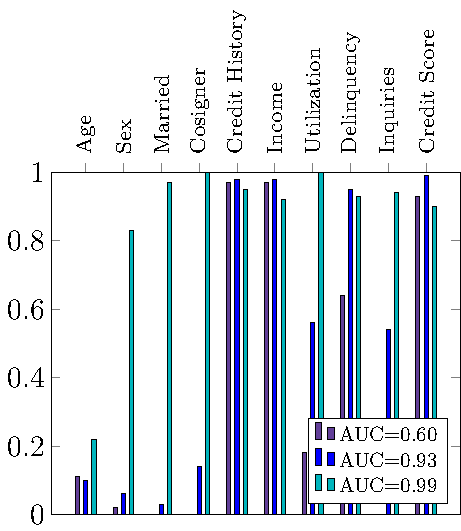
\includegraphics[width=.28\textwidth]{Figures/sec4_4_mlp_auc_shap-figure0.pdf}}%
                \label{subfig:mlp_avg_shap_sign_accs}%
            }\hspace{1cm}
            \subfloat[SHAP Concordance]{%
                 \raisebox{.05cm}{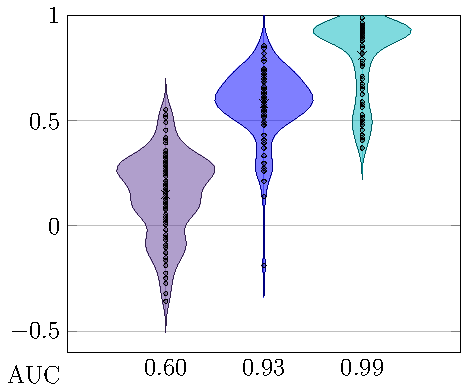
\includegraphics[width=.28\textwidth]{Figures/sec4_4_mlp_auc_shap-figure1.pdf}}%
                \label{subfig:mlp_auc_shap_spearmans}%
            }\hspace{1cm}
            \subfloat[SHAP Relevance]{%
                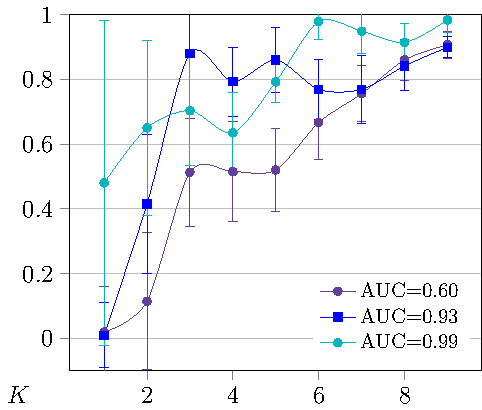
\includegraphics[width=.28\textwidth]{Figures/sec4_4_mlp_auc_shap-figure2.pdf}%
                \label{subfig:mlp_auc_shap_recalls}%
            }\\
            \subfloat[LIME Directionality]{%
                \raisebox{.2cm}{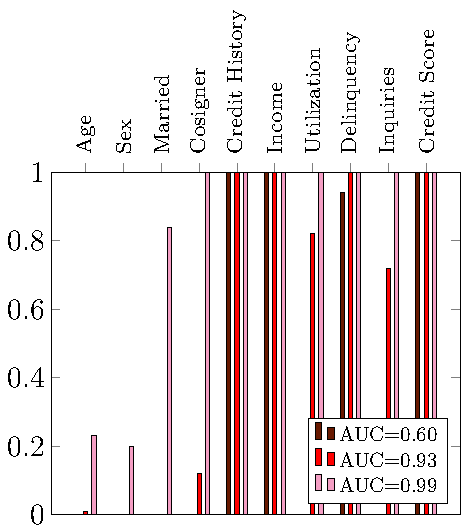
\includegraphics[width=.28\textwidth]{Figures/sec4_4_mlp_auc_lime-figure0.pdf}}%
                \label{subfig:mlp_auc_lime_sign_accs}%
            }\hspace{1cm}%\hfill
            \subfloat[LIME Concordance]{%
                \raisebox{.05cm}{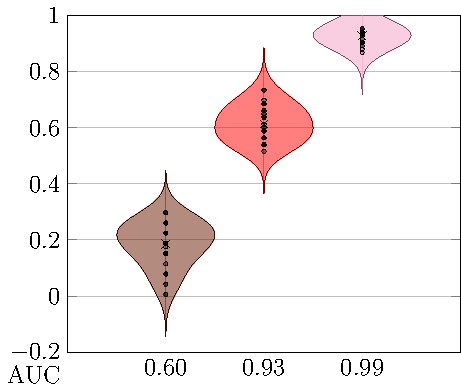
\includegraphics[width=.28\textwidth]{Figures/sec4_4_mlp_auc_lime-figure1.pdf}}%
                \label{subfig:mlp_auc_lime_spearmans}%
            }\hspace{1cm}
            \subfloat[LIME Relevance]{%
                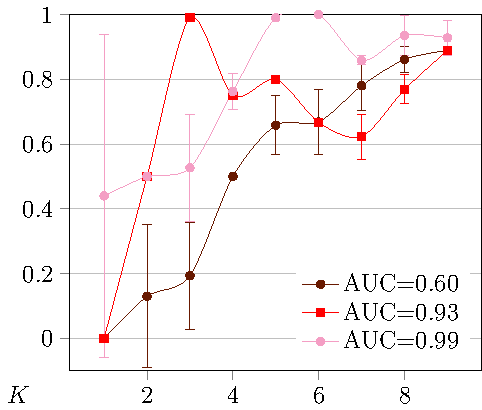
\includegraphics[width=.28\textwidth]{Figures/sec4_4_mlp_auc_lime-figure2.pdf}%
                \label{subfig:mlp_auc_lime_recalls}%
            }\\
            \caption{Comparisons of results for our three metrics for SHAP and LIME when explaining $\mathcal{M}_1$ with AUC=.6, $\mathcal{M}_2$ with AUC=0.92, and $\mathcal{M}_3$ with AUC=.99}
            \label{fig:mlp_auc_increase}
        \end{figure}

    
    %https://stats.stackexchange.com/questions/15011/generate-a-random-variable-with-a-defined-correlation-to-an-existing-variables
    \subsubsection{Role of Feature Independence}
        \label{sec:role_of_correlation}
        The primary goal of training routines for predictive machine learning algorithms is to construct a mapping from the inputs to the outputs in a dataset that produces correct labels. However, a side effect of this focus on predictive performance is that ML models tend to overvalue features that provide information about multiple other features, as these are strong predictors of the target \citep{scholkopf2021toward}. Therefore, the dependence of features can skew their perceived importance in a model, and this importance may be estimated by an explainer and subsequently used to draw incorrect conclusions about the data.

        In real-world scenarios, features are typically interdependent. Thus, while the ideal model might rely predominantly on some features to determine the correct label, $\mathcal{M}$ might rely more on other features. Consequently, $\mathcal{M}$ can arrive at the same predictions through an alternate mapping. Complicating this issue is the fact that, regardless of opinions on the significance of dependent variables, machine learning models tend to overvalue features that provide information about multiple other features, as these are strong predictors of the target. Post hoc explainers then interpret the importance of such features in various ways, further muddying the understanding of feature relevance within an ML model.
     %        Underlying all natural phenomena is a tangled web of mechanisms which move together to produce what we can perceive and measure. Consider, for example, the following ground truth model depending on features $X_1$ and $X_2$. Let $\mathcal{G}(X_1,X_2) = \alpha_1 X_1 + \alpha_2 X_2$. In this case, $\alpha_1$ and $\alpha_2$ represent the unambigious separate effects of $X_1$ and $X_2$ on $Y$. However, adding a dependence relation such as $X_2 = \gamma X_1 + \epsilon$ makes importance of $X_1$ and $X_2$ on $Y$ unclear; it is only a matter of opinion and context whether $X_2$ is important at all.

         To demonstrate how interdependent features can impact data-alignment, we generate a modified version of the dataset from Section \ref{sec:data_generation} with mutually independent features. Specifically, in this revised dataset, ``Credit Score" is independent of other features rather than being derived from ``Credit Utilization," ``Credit Inquiries," ``Delinquencies," and ``Credit History". Additionally, ``Cosigner"  is now modeled as a Bernoulli-distributed random variable which is independent of ``Married". In this case, the marginal effects $\boldsymbol{\beta}$ of $\mathcal{G}$ match the coefficients from Equation (\ref{eqn:gt}). %We normalize the SHAP values in an effort to show how feature independence can affect explanations obtained from SHAP, in spite of its inherent data-misalignment.
        

        We clarify the role of feature independence by comparing the alignment of explanations of models trained on the revised dataset with mutually independent features and the original dataset with interdependent features. We will begin analyzing our results by considering overall data-alignment. Then we examine alignment with respect to ``Married" in order to give an example of how alignment with respect to a feature can be lower if that feature is made to be highly correlated with another feature.
        
        Our experiment showed that by making ``Credit Score" and ``Cosigner" independent, data-alignment increased overall and with respect to ``Credit Score" and ``Cosigner" in particular. Figures \ref{fig:shap_corr_accs} and \ref{fig:lime_corr_accs} show that both SHAP and LIME's directionality for ``Cosigner" improved by making it independent of ``Married". SHAP's directionality for ``Credit Score" also improved substantially. The most notable results come from the significant increases in relevance and concordance, especially for LIME.
        \begin{figure}[h]
            \subfloat[SHAP Directionality]{%
                \raisebox{.2cm}{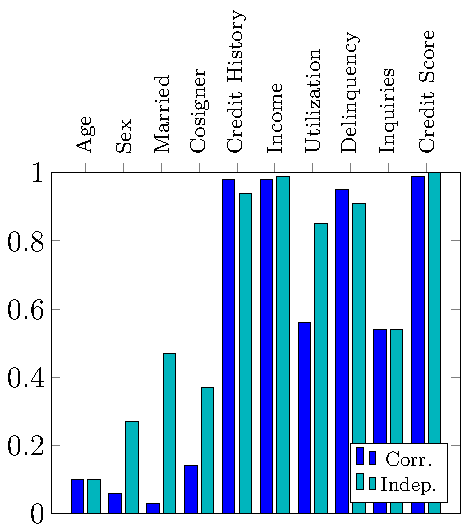
\includegraphics[width=.28\textwidth]{Figures/sec4_3_corr_shap-figure0.pdf}}%
                \label{fig:shap_corr_accs}%
            }\hspace{1cm}%\hfill
            \subfloat[SHAP Concordance]{%
                \raisebox{.05cm}{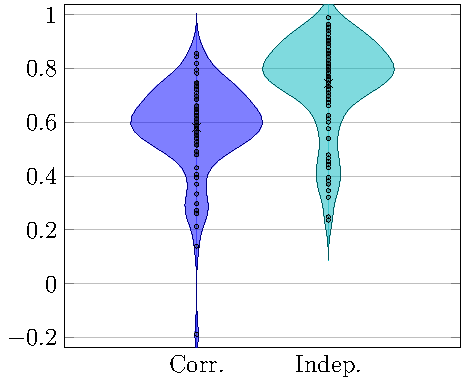
\includegraphics[width=.28\textwidth]{Figures/sec4_3_corr_shap-figure1.pdf}}%
                \label{fig:shap_corr_spearmans}%
            }\hspace{1cm}%\hfill
            \subfloat[SHAP Relevance]{%
                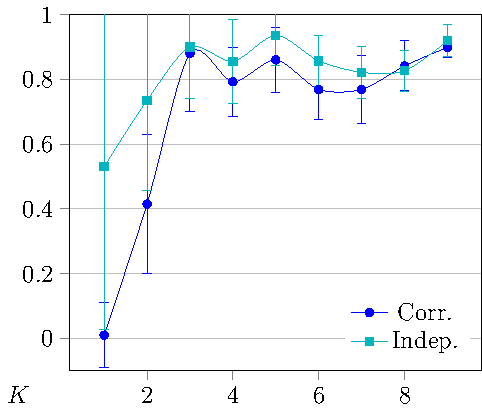
\includegraphics[width=.28\textwidth]{Figures/sec4_3_corr_shap-figure2.pdf}%
                \label{fig:shap_corr_recalls}%
            }\\
            \subfloat[LIME Directionality]{%
                \raisebox{.2cm}{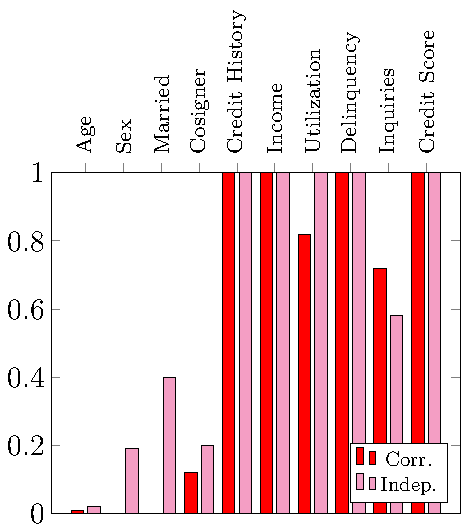
\includegraphics[width=.28\textwidth]{Figures/sec4_3_corr_lime-figure0.pdf}}%
                \label{fig:lime_corr_accs}%
            }\hspace{1cm}%\hfill
            \subfloat[LIME Concordance]{%
                \raisebox{0cm}{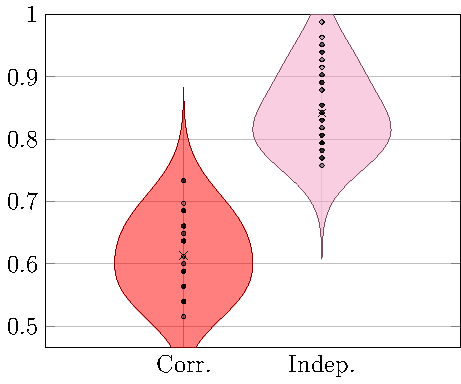
\includegraphics[width=.28\textwidth]{Figures/sec4_3_corr_lime-figure1.pdf}}%
                \label{fig:lime_corr_spearmans}%
            }\hspace{1cm}%\hfill
            \subfloat[LIME Relevance]{%
                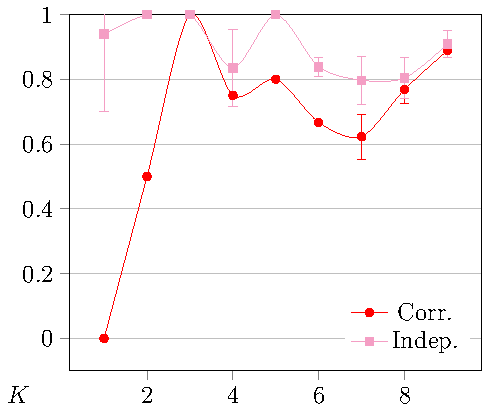
\includegraphics[width=.28\textwidth]{Figures/sec4_3_corr_lime-figure2.pdf}%
                \label{fig:lime_corr_recalls}%
            }\\
            \caption{Comparison of faithfulness of explanations of models trained on data with independent features versus data with two strongly correlated features.}
            \label{fig:lime_shap_colinear}
        \end{figure}
 SHAP saw significant gains in relevance for all $k$ except $k=3,8,9$ (see  Figure \ref{fig:shap_corr_recalls}) as well as a large leap in concordance. Figure \ref{fig:lime_corr_recalls} shows that LIME was adept at identifying the top $k=1,2,3$ most important features when the features were independent while it could rarely (or never) do so when the features were not independent. Its mean concordance was also larger by about $.2$. It is evident from our results that the interdependence of features obfuscates explainers and leads to incorrect feature importance.    

    %\paragraph{Lower Alignment For Correlated Features In Particular}
            %We showed that, when explaining predictions of models with similar predictive performance trained on two similar datasets that differ by virtue of their features being mutually independent (or not), the explanations of the model trained on the data with mutually independent features were more data aligned. One of the differences between the two datasets was that in the original, being married increased the chance that an applicant had a cosigner, while in the variant they were independent. In this experiment, we will show how an example of how marital status influencing cosigner posession, a more important feature for loan approval, is associated with lower data-alignment of explanations with respect to marital status in particular.
        
            Figure \ref{fig:marital_sign_accs} shows bar plots of directionality for ``Married" by SHAP and LIME before and after making the ``Cosigner" depend on ``Married". The bar plots show that the addition of dependencies between features is associated with a loss of the ability to give ``Married" the correct sign for both SHAP and LIME. Additionally, Figure \ref{fig:marital_rank_diff} shows the distributions of the absolute differences between the given and correct rank for ``Married" before and after the introduction of correlation. We see that for both SHAP and LIME, the average ranking error for ``Married" is much smaller when the features are mutually independent than otherwise. These results suggest that it may be more difficult for explainers to extract correct information about the individual marginal effects of interdependent features.
            \begin{figure}[ht!]
                \centering
                \begin{subfigure}{.28\textwidth}
                  \centering
                  \captionsetup{justification=centering}
                  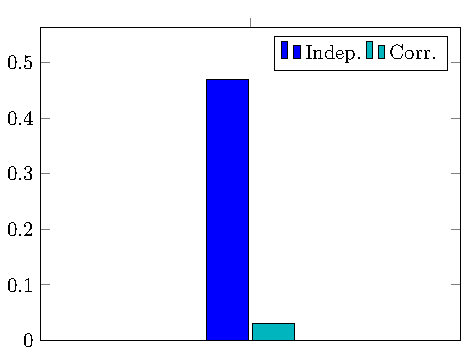
\includegraphics[width=\textwidth]{AppendixFigures/apx_marital-figure1.pdf}%{Figures/fig_age_col.pdf}%{Figures/lime_spearman_colinear.png}
                                %\includegraphics[width=.9\linewidth]{Figures/lime_shap_Spearman_magnitude.png}
    
                  \caption{SHAP}%Spearman rank correlations of ranked feature importance magnitudes from LIME against the true ranked magnitudes from $\mathcal{G}$.}
                   \label{fig:marital_sign_accs_shap}
                \end{subfigure}%
                \hspace{3cm}
                \begin{subfigure}{.28\textwidth}
                  \centering
                     \captionsetup{justification=centering}
                  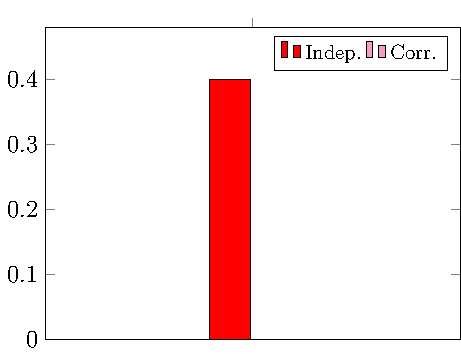
\includegraphics[width=\textwidth]{AppendixFigures/apx_marital-figure0.pdf}%{Figures/fig_score_col.pdf}%{Figures/shap_spearman_colinear.png}
    
                  %\includegraphics[width=.9\linewidth]{Final_Figures/fig9b.png}%{Figures/shap_spearman_colinear.png}
                  \caption{LIME}%Spearman rank correlations of signed feature importance magnitudes from SHAP and LIME against the true ranking from $\mathcal{G}$.}
                   \label{fig:marital_sign_accs_lime}
                \end{subfigure}
                
                \caption{Bar charts showing how SHAP and LIME (almost) never can correctly identify the sign of ``Married" when it is used to determine ``Cosigner".}%rankings of age and credit score change from when being independent to when credit score becomes a function of age}
                \label{fig:marital_sign_accs}
            \end{figure}

            \begin{figure}[ht!]
                \centering
                \begin{subfigure}{.28\textwidth}
                  \centering
                  \captionsetup{justification=centering}
                  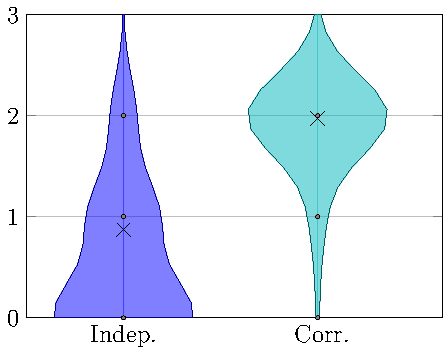
\includegraphics[width=\textwidth]{AppendixFigures/apx_marital-figure2.pdf}%{Figures/fig_age_col.pdf}%{Figures/lime_spearman_colinear.png}
                                %\includegraphics[width=.9\linewidth]{Figures/lime_shap_Spearman_magnitude.png}
    
                  \caption{SHAP}%Spearman rank correlations of ranked feature importance magnitudes from LIME against the true ranked magnitudes from $\mathcal{G}$.}
                   \label{fig:marital_rank_diff_shap}
                \end{subfigure}%
                \hspace{3cm}
                \begin{subfigure}{.28\textwidth}
                  \centering
                     \captionsetup{justification=centering}
                  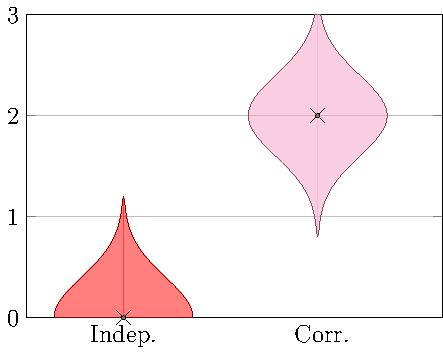
\includegraphics[width=\textwidth]{AppendixFigures/apx_marital-figure3.pdf}%{Figures/fig_score_col.pdf}%{Figures/shap_spearman_colinear.png}
    
                  %\includegraphics[width=.9\linewidth]{Final_Figures/fig9b.png}%{Figures/shap_spearman_colinear.png}
                  \caption{LIME}%Spearman rank correlations of signed feature importance magnitudes from SHAP and LIME against the true ranking from $\mathcal{G}$.}
                   \label{fig:marital_rank_diff_lime}
                \end{subfigure}
                
                \caption{Violin plots showing the differences between the given rank and true rank of ``Married" depending on whether ``Married" influences ``Cosigner". Lower is better.}%rankings of age and credit score change from when being independent to when credit score becomes a function of age}
                \label{fig:marital_rank_diff}
            \end{figure}

  
    
    \subsection{Discussion}
            Since researchers cannot directly access the ground truth model $\mathcal{G}$ and can only interact with an intermediary machine learning model $\mathcal{M}$, the process of explanation is bifurcated into two distinct stages: the prediction stage and the explanation stage. To generate explanations that accurately reflect the marginal effects, one must navigate challenges that may arise in either stage, necessitating additional assumptions about the data, $\mathcal{M}$, and the explanation tool $\mathcal{E}$. Crucially, $\mathcal{E}$ must possess the ability to accurately capture information regarding the marginal effects. The discussion in Section \ref{sec:theoretical_considerations} describes theoretically why SHAP and LIME are inherently incapable of extracting even qualitative information (e.g. the sign) about the true marginal effects. In addition, even if we presume $\mathcal{E}$'s competence in recovering the actual marginal effects, it is essential for $\mathcal{M}$ to closely approximate $\mathcal{G}$, ensuring that information about the marginal effects is indeed present within $\mathcal{M}$. Insights from Section \ref{sec:causes_of_misalignment} indicate that $\mathcal{M}$'s ability to achieve high predictive accuracy, especially when trained on data featuring mutually independent variables, significantly facilitates the extraction of the marginal effects. However, \textbf{SHAP and LIME being data-misaligned appears to be a general phenomenon}, which worsens with \textit{low predictive performance of the machine learning model, dependence of features, and the large number of features}. 


% \section{Inconsistency of Post Hoc Explanations}
%     \label{sec:inconsistency}
%     Another major issue post hoc explanations  suffer from is inconsistency, which refers to one or more post hoc explainers providing conflicting information about the marginal effects. Inconsistency is a source of confusion and frustration because without sufficient domain knowledge, misaligned explanations cannot be distinguished from aligned ones. Inconsistency can facilitate generation of invalid hypotheses and invalid inference because users without domain knowledge that are not able to account for inconsistency may be forced to make arbitrary selections of explanations. 

%     Explanation inconsistency has to do with the \textit{model being explained} (i.e., $\mathcal{M}$) and the \textit{explainers} (i.e., $\mathcal{E})$. Fixing one explainer and varying $\mathcal{M}$  may yield differing hypotheses about the marginal effects. This variation is due to the different ways in which models capture and approximate the ground truth ($\mathcal{G}$) and their unique decision-making processes, which can significantly diverge even when their predictions appear similar. Factors such as the dataset characteristics and the internal mechanisms and structures of $\mathcal{M}$ influence these outcomes. Conversely, for a fixed $\mathcal{M}$, explanations could still vary due to inherent differences among the explainers or differing configurations of an explainer's hyperparameters. We provide in Appendix Section \ref{apx_sec:appendix_inconsistency} a set of experiments that demonstrate how inconsistency arises with different combinations of explanation methods and models. For example, we show that both the feature rankings and signs from pairs of SHAP and LIME explanations of the same prediction are usually different.

%     In Appendix Section \ref{apx_sec:instability} we also explore a more general form of inconsistency known as instability. Inconsistency of explanations for similar inputs is called instability. Instability can manifest when, e.g., two applicants with similar profiles get different explanations and can lead to uncertainty about which explanation better represents the marginal effects and possibly unfounded suspicions that the decision process is unfair. 


          
%           %At any rate, the issue of inconsistency makes it difficult to justify any one explanation or pipeline configuration if one does not have sufficient domain knowledge, since alternatives abound with equal plausibility. It follows that researchers who wish to use SHAP or LIME to generate hypotheses about their data should take care in doing so. Researchers should be reticent if considering proclaiming that they have identified some novel phenomena via post hoc feature importance values since such novelty could merely be an artifact of inconsistency. Inconsistency thus facilitates generation of invalid hypotheses and invalid inference because users without domain knowledge that are not able to account for inconsistency are forced to make arbitrary selections of explanations. %We also discussed how the volatility of the decision boundary of $\mathcal{M}$ in comparison to the volatility of the decision boundary of $\mathcal{G}$ affects explanation stability. Explaining an underfit $\mathcal{M}$ as part of a fairness audit of $\mathcal{G}$ could cause unfairness to go unnoticed. Conversely, explanations of similar inputs to an overfit $\mathcal{M}$ could be dissimilar and cause confusion and make neither explanation justifiable. %Consider, for example, how Figure \ref{fig:lime_rankings_mag} shows that LIME may indicate that the least important feature is the most important (and vice versa).
         



\section{Mitigation Strategies}
    \label{sec:mitigation_strategies}
    In this section, we use the results of our experiments and the implications of the theoretical results from Section \ref{sec:theoretical_considerations} to propose and test some simple mitigation strategies for misalignment. The strategies we propose here are meant to be sufficiently simple to understand and use such that they form a platform for further exploration and experimentation. We soften the impact of our choices for the data and model in this section by using the version of our dataset with mutually independent features and an NN with accuracy and test set ROC AUC equal to $.99$ in each experiment, unless otherwise stated. To begin the section, we will introduce the criteria we use to test if a strategy improves data-alignment over a baseline with respect to directionality, concordance, and relevance. Then we describe and demonstrate our mitigation strategies, starting with those that are specific to SHAP or LIME and concluding with generally applicable strategies. Using our definitions of improvement, the mitigation strategies we propose are all effective in at least one of the metrics. We provide results for less effective mitigation strategies in the Appendix. 

    %\subsection{Mitigation Strategies for misalignment}
    %\label{sec:incorrectness_mitigation} %\textcolor{red}{move this to the end of section 4. this is the mitigation strategy for incorrectness}
    
        %We propose a few intuitive mitigation strategies for explanation faithfulness based on data pre-processing and, model training, and explainer hyperparameters. We first demonstrate the truth of Corrolaries 1 and 2 from Section \ref{sec:theoretical_considerations}. We then verify that ensuring both that $\mathcal{M}$ has high test set accuracy and that its training data has no unobserved, correlated, or confounded features is associated with increased explanation quality. The next strategy involves ensuring that $\mathcal{M}$ has high test set ROC AUC. The final strategy involves ensuring that the underlying model of $\mathcal{E}$ correctly classifies the input being explained. When demonstrating the first, third, and fourth strategies, the training data do not have unobserved, correlated, or confounded features in order to isolate the roles of $\mathcal{E}$ and $\mathcal{M}$. 
    \subsection{Testing Improvement}
        \label{sec:improvement}
        This section introduces the hypothesis testing framework that we use to characterize whether an explanation method $\mE^\prime$ improves over a baseline explanation $\mE$ in terms of directionality, concordance, and relevance. All details, including statements of the null and alternative hypotheses we use, can be found in the Appendix.
        
        
        The underlying idea for our tests for improvement is to test if the mean(s) of metrics of interest is (are) higher for $\mE^\prime$ than for $\mE$ using Wilcoxon signed-rank tests on the location of mean of differences from a matched sample(s).
        %When testing for improvement of consistency of feature importance signs, we use one-sided McNemar tests for whether pairs of the pipeline with the mitigation strategy applied and baseline disagree on feature importance signs at the same rate. 
        All of our tests are performed with a significance level of $\alpha=.05$. 
        
        We formulate a rather strict characterization of improvement of $\mE^\prime$ over $\mE$ with respect to directionality and relevance. Our tests for directionality and relevance are meant to capture when $\mE^\prime$ has a statistically significant improvement over $\mE$ in at least one respect and is not significantly worse than $\mE$ in any respect. What this means for directionality is that directionality must have a statistically significant increase for at least one feature and no statistically significant decrease for any feature. Similarly, for relevance, it means that the mean relevance of $\mE^\prime$ must be significantly larger than that of $\mE$ for at least one $k$, and not significantly smaller for any $k$. 
        
        
     


    \subsection{Explainer Specific Strategies}
        Before discussing general-use strategies, we will present three strategies applicable only to SHAP or LIME (but not both). 

            \subsubsection{Normalizing The Shapley Value}
                As discussed in Section \ref{sec:theoretical_considerations}, it follows directly from the theory underlying SHAP that SHAP explanations do not yield the marginal effect values $\boldsymbol{\beta}$. It is therefore worthwhile to seek practical ways to modify our usage of SHAP. Since equation \ref{eqn:shap_gt} showed that SHAP returns $e_{\text{SHAP}}(\mathbf{x}^{(i)})=\boldsymbol{\beta}^T(\mathbf{x}^{(i)} - \bar{\mathbf{x}})$ instead of $\boldsymbol{\beta}$, we proposed in Section \ref{sec:theoretical_considerations} to instead take the importance of feature $j$ to be $e_{\text{SHAP}}(x^{(i)}_j) / (x^{(i)}_j - \bar{x}_j)$ where $\bar{x}_j$ is the empirical mean of feature $j$ from the training data because this expression should be approximately $\beta_j$. Our experiments confirmed the advantage of this strategy: Figure \ref{fig:shap_dividex_corr} showed that unmodified SHAP explanations perform about as well as random explanations with respect to our three metrics while the normalized SHAP explanations performed significantly better in all three metrics. Therefore, all strategies involving SHAP will first make use of the normalization scheme by default.

                %In addition, the normalized SHAP explanations were more consistent across individuals (recall that Figure \ref{fig:shap_dividex_spearmans} showed that the concordance distribution for normalized SHAP explanations had a significantly smaller region of support which, importantly, was centered at a larger value than the mean concordance of the unmodified SHAP explanations). 
                %%Since these results were produced using the version of our dataset with correlated features, we additionally provide a comparison of SHAP without and with normalization when the input features are independent in Appendix Section \ref{apx_sec:shap_norm_indep}.



        
        \subsubsection{Increasing $\nu$ and $n$ for LIME } 
            \label{sec:lime_params}
            Corollary 1 from Section \ref{sec:theoretical_considerations} implies that LIME's kernel bandwidth $\nu$ and number of perturbed samples $n$ need to be large in order for $e_{\text{LIME}}(x_j)$ to be close to $\boldsymbol{\beta}$, so this section will experiment with how their respective sizes affect explanation quality. In our experiment, we compare the data-alignment of explanations from LIME explanations using the default choices of $\nu = .75\sqrt{d}$ (where $d$ is the number of features) and $n=1000$ used in the official LIME implementation \citep{ribeiro16lime} with LIME explanations which use the larger values $\nu=n=10000$. 
            
            Figure \ref{fig:lime_tuning} shows that increasing the number of samples $n$ and the kernel bandwidth $\nu$ improves directionality, concordance, and relevance. Although the results for ``Credit History," ``Credit Score," ``Delinquency," ``Income," ``Inquiries," and ``Utilization" were identical before and after the strategy was applied, we found that increasing $\nu$ and $n$ improved directionality  significantly for the remaining features, as our Wilcoxon tests for equal signs accuracies had p-values of $0.01$ for ``Age," $2.34e-3$ for ``Cosigner," and $p<.001$ for ``Sex." The larger $\nu$ and $n$ also resulted in pairs of rankings whose concordances were both larger on average; our test for equally consistent rankings had $p<.001$. %The plot of $\text{relevance}_k$ shows that using $\nu=n=10000$ netted a strict advantage for correctly ranking the features which were not the most or least important. That is, for $k=1$ the results were identical and for $k=2,8$ we fail to reject the null hypothesis of equal relevances with a p-values of $0.08$ and $0.12$ respectively, but we do reject the null hypotheses for $k=3,\ldots,7$ with p-values of $9.14e-5$, $4.56e-4$, $1.71e-7$, $2.64e-11$, and $5.90e-12$.
        
            \begin{figure}[ht!]
                \centering
                \begin{subfigure}[t]{.28\textwidth}
                  \centering
                  \captionsetup{justification=centering}
                      \raisebox{.2cm}{\includegraphics[width=\textwidth]{Figures/sec4_4_LIME-figure0.pdf}}%{Figures/lime_shap_Spearman_magnitude.png}
    
                  \caption{Directionality}%Spearman rank correlations of feature importance magnitudes from SHAP and LIME against the true ranking from $\mathcal{G}$. }
                   \label{fig:lime_tuning_sign_accs}
                \end{subfigure}%
                \hspace{1cm}
                \begin{subfigure}[t]{.28\textwidth}
                  \centering
                   \captionsetup{justification=centering}
                  \includegraphics[width=\textwidth]{Figures/sec4_4_LIME-figure1.pdf}%{Figures/lime_shap_Spearman_signed.png}
                  \caption{Concordance}%Spearman rank correlations of signed feature importance from SHAP and LIME against the true ranking from $\mathcal{G}$.}
                   \label{fig:lime_tuning_spearmans}
                \end{subfigure}
                \hspace{1cm}
                \begin{subfigure}[t]{.28\textwidth}
                  \centering
                   \captionsetup{justification=centering}
                \includegraphics[width=\textwidth]{Figures/sec4_4_LIME-figure2.pdf}%
                \caption{Relevance}%The average and standard error of recall of SHAP and LIME when attempting to capture the top K most important features to $\mathcal{G}$ when explaining $\mathcal{M}$, for varied $K=1,2,3,...$ number of features.}
                \label{fig:lime_tuning_recalls}
                \end{subfigure}
                \caption{Comparison of LIME explainer with default settings $\nu=.75\sqrt{d}\simeq 2.37,\ n=1000$ versus $\nu=n=10000$ with respect to our three metrics}
               \label{fig:lime_tuning}
            \end{figure} 
% \tw{Figure 8c looks so weird. How come it's a decreasing curve?}
            \subsubsection{Averaging Explanations of One Model by Different Explainers}
            \label{sec:averaging_one_explainer}
            Since there exists randomness in LIME (the random seed, the sampling, etc), the feature importance may not be exactly the same if LIME is run multiple times. This is a problematic property of LIME since its explanations are inconsistent \citep{alvarez18robustness} as a result of this randomness. 
        However, we propose that it can actually be leveraged into an advantage. Each explanation likely has at least a modicum of truth, and so an aggregation strategy for explanations may increase the signal-to-noise ratio. We propose here one simple realization of this general idea. Given one ML model $\mathcal{M}$ and instance $\mathbf{x}$, we leverage the abundance of possible LIME explanations of $\mathcal{M}(\mathbf{x})$ by averaging the feature importance values given by a set of LIME explainers with different random seeds.
        
            We compare explanations averaged from 100 LIMEs with explanations from one LIME on  $m=100$ applications. %The averaged explanation for each applicant is constructed by averaging over the feature importance values from 100 LIME explanations of the applicant, where the 100 explainers are created using random seeds $1,\ldots,100$ and default settings. .  %We repeat this with $\nu=n=10000$. 
            Our statistical tests of improvement concluded that directionality, concordance, and relevance were significantly improved by using averaged instead of single LIME explanations. Averaging LIME explanations resulted in an enhanced ability to find the sign of ``Age", ``Sex", ``Married" and ``Cosigner" (see Figure \ref{fig:lime_avg_sign_accs}). The mitigation did not change the assignment of the other features but we were able to reject the null hypothesis of equal sign accuracies for ``Age," ``Cosigner," ``Married," and ``Sex" all with $p<.001$. %$3.32e-3$, $2.34e-3$, $3.17e-5$, and $2.12e-6$, respectively.
            Moreover, the concordances  of the averaged explanations were higher than single explanations; we rejected the null hypothesis of equal concordances with $p<.001$.%a p-value of $7.39e-12$. %Figure \ref{fig:lime_avg_recalls} also shows that the averaged explanations were more likely to identify the features which were not the most or least important. 

            % \begin{table}[]
            % \centering
            % \begin{tabular}{|l|l|l|l|l|l|l|l|l|l|}
            % \hline
            % Age  & Cosigner & Credit History & Credit Score & Delinquency & Income & Inquiries & Married & Sex & Utilization \\ \hline
            % 0.98 & 1.20e-7   & n/a            & n/a          & n/a         & n/a    & 0.50      & 1.11e-4 & .12 & n/a         \\ \hline
            % \end{tabular}
            % \caption{p-values for improvement to consistency of feature importance signs by using averaged LIME explanations. Values are listed as ``n/a" if both pairs of explanations always found the correct sign for the corresponding feature.}
            % % \label{tab:lime_avg_sign_con}
            % \end{table}
                             
            \begin{figure}[!h]
            \centering
                \begin{subfigure}[t]{0.28\textwidth}
                \centering
                \raisebox{.2cm}{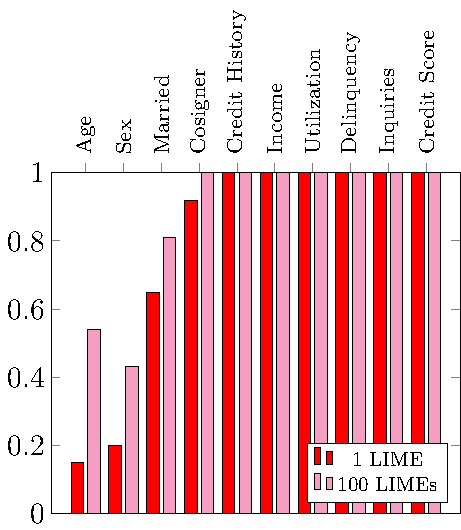
\includegraphics[width=\textwidth]{Figures/sec5_2_lime_avg-figure0.pdf}}
                \caption{Directionality} \label{fig:lime_avg_sign_accs}
            \end{subfigure}\hspace{1cm}
            \begin{subfigure}[t]{0.28\textwidth}
                \centering
                \raisebox{.05cm}{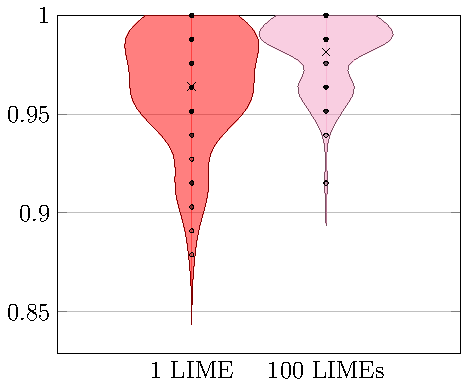
\includegraphics[width=\textwidth]{Figures/sec5_2_lime_avg-figure1.pdf}}
                \caption{Concordance} \label{fig:lime_avg_spearmans}
            \end{subfigure}\hspace{1cm}
             \begin{subfigure}[t]{0.28\textwidth}
                \centering
                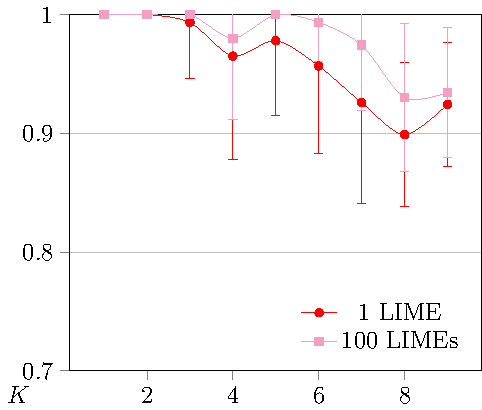
\includegraphics[width=\textwidth]{Figures/sec5_2_lime_avg-figure2.pdf}
                \caption{Relevance}
                \label{fig:lime_avg_recalls}
            \end{subfigure}
            \caption{Comparisons of results for our three metrics for  explanations of an NN $\mathcal{M}$ by 1 LIME explainer versus those created by averaging the feature importance values of 100 LIME explanations of $\mathcal{M}$}\label{fig:lime_avg}
            \end{figure}

                
            %It was also the case that the averaging routine significantly improved consistency. To obtain this result, we created another set of average explanations from 100 more LIME explainers using random seeds $101,\ldots,200$, and tested whether the signs and rankings were more consistent between the two sets of averaged explanations compared to the signs and rankings of the two individual LIME explainers. We rejected the null hypotheses of our tests for equal consistency of feature importance signs in favor of improvement for ``age", ``cosigner", and ``married" all with $p<.001$.%of  $8.65e-3$, $1.20e-7$ and $1.11e-4$, respectively.
            %There was no change for ``credit  history", ``credit score", ``delinquency", ``income", and ``utilization" because both methods were perfect in each case.  With a p-value of $7.60e-15$, we rejected the null hypothesis of our Wilcoxon test that the means of the two concordance distributions are equal in favor of the alternative hypothesis that the mean of the concordance distribution from the averaged explanations is larger. That this is the case is also visually evident from Figure \ref{fig:lime1_v_100_incon}; the concordance distribution of the averaged explanations was more concentrated near 1 and its tail was also shorter. 

            % \begin{figure}[ht!]
            %     \centering
            %     %\begin{subfigure}{.3\textwidth}
            %       \centering
            %       \captionsetup{justification=centering}
            %       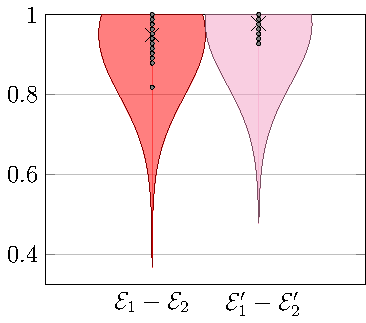
\includegraphics[width=.28\textwidth]{Figs/sec5_2_lime_avg2-figure3.pdf}
            %       \caption{Comparison of concordances between explanations from pairs of individual LIME explainers and between pairs of averaged explanations from two sets of 100 LIME explainers.}%Spearman rank correlations of ranked feature importance magnitudes from LIME against the true ranked magnitudes from $\mathcal{G}$.}
            %        %\label{fig:lime_income}
            %     %\end{subfigure}%
            %     %\caption{}%Violin plots of feature importance values for \emph{income} from SHAP and LIME for cases when \emph{income} is unconfounded and confounded by the unobserved social support feature}
            %     \label{fig:lime1_v_100_incon}
            % \end{figure}
                
    \subsection{General Strategies}
        We now provide three general strategies that can be applied to both SHAP and LIME to produce explanations that are more data-aligned. Note that we have been and will continue using normalized Shapley values, since default SHAP explanations are not better than random with respect to data-alignment. %To show the utility of these strategies for SHAP, we will use normalized SHAP values in each the experiments below. 

        \subsubsection{Optimizing the Tradeoff between Complexity and Predictive Power}
            \label{sec:decreasing_complexity}
            The size of the hypothesis space, which refers to the set of all possible models that can be considered for a given dataset, for any dataset of practical utility is unimaginably large, making model selection for prediction tasks difficult at the outset. Further complicating the problem of model selection is there can be many models with similar predictive performance, known as the Rashomon Set Theory \citep{semenova22rashomon}. Given that notions of complexity such as parameter count are basic distinguishing properties of models, statistics literature on parsimony in curve fitting often appeals to Occam's razor - plurality should not be posited without necessity,  positing that simpler models are more likely to be correct than complex ones \citep{popper2005logic}.

            
            For this reason, we design a mitigation strategy which takes into account  the complexity of $\mathcal{M}$. Since we established in Section \ref{sec:role_of_predictive_power} an association between the predictive performance of $\mathcal{M}$ and the alignment of post hoc explanations of $\mathcal{M}$ with respect to $\mathcal{G}$; this mitigation strategy proposes to ensure that $\mathcal{M}$ has both good predictive performance and minimal complexity. %The labels predicted by $\mathcal{M}$ (after thresholding its output probabilities) agreeing with those in the test set is an incomplete representation of faithfulness to $\mathcal{G}$; even if $\mathcal{M}$ had 100\% training and testing accuracy on data with no measurement error, this does not mean $\mathcal{M}=\mathcal{G}$.  Thus, it is worth making an effort not to over-parameterize $\mathcal{M}$. %\tw{The explanation should be moved to earlier this paragraph. WE can use the argument of Ocam's razor, that low complexity is generally preferred. This point should be given a deeper discussion before proposing to get ``minimal complexity"} 
            To carry out this strategy, one can iteratively train and evaluate models of successively lower complexity and stop the procedure once the reduction of complexity leads to a substantial reduction in predictive performance. 
   \begin{figure}[t!]
            \subfloat[SHAP Directionality]{%
                \raisebox{.2cm}{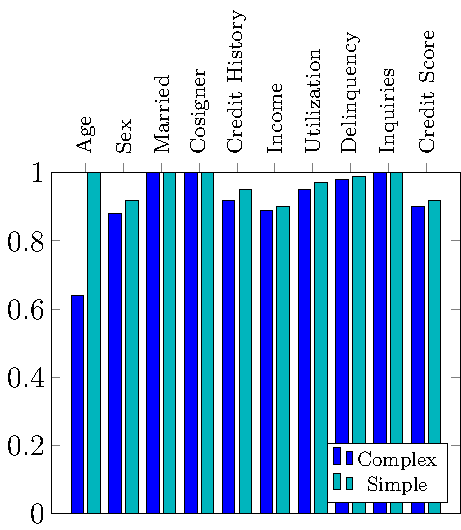
\includegraphics[width=.28\textwidth]{Figures/sec5_mlp_complexity_shap-figure0.pdf}}%
                \label{subfig:decreasing_complexity_shap_sign_accs}%
            }\hspace{1cm}
            \subfloat[SHAP Concordance]{%
                \raisebox{.05cm}{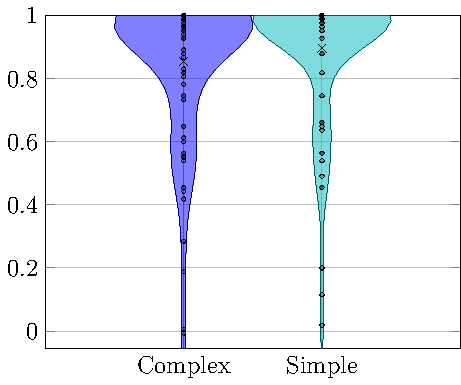
\includegraphics[width=.28\textwidth]{Figures/sec5_mlp_complexity_shap-figure1.pdf}}%
                \label{subfig:decreasing_complexity_shap_spearmans}%
            }\hspace{1cm}
            \subfloat[SHAP Relevance]{%
                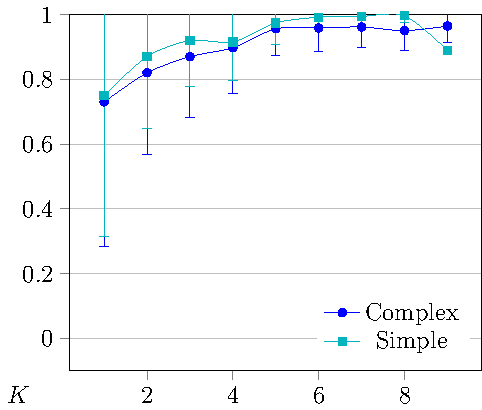
\includegraphics[width=.28\textwidth]{Figures/sec5_mlp_complexity_shap-figure2.pdf}%
                \label{subfig:decreasing_complexity_shap_recalls}%
            }\\
            \subfloat[LIME Directionality]{%
                \raisebox{.2cm}{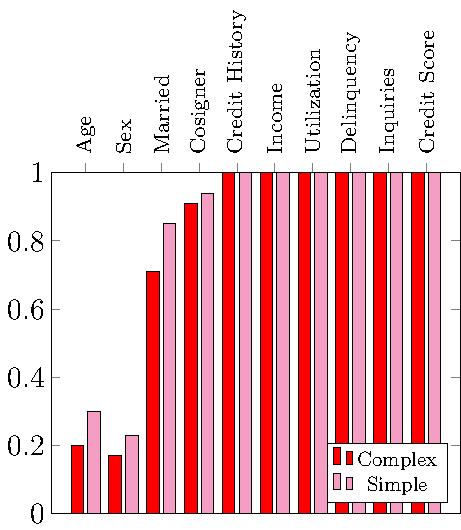
\includegraphics[width=.28\textwidth]{Figures/sec5_mlp_complexity_lime-figure0.pdf}}%
                \label{subfig:decreasing_complexity_lime_sign_accs}%
            }\hspace{1cm}
            \subfloat[LIME Concordance]{%
                \raisebox{.05cm}{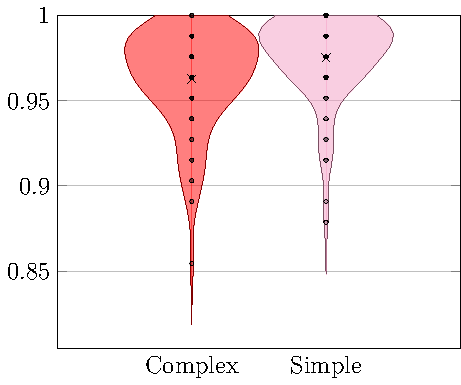
\includegraphics[width=.28\textwidth]{Figures/sec5_mlp_complexity_lime-figure1.pdf}}%
                \label{subfig:decreasing_complexity_lime_spearmans}%
            }\hspace{1cm}
            \subfloat[LIME Relevance]{%
                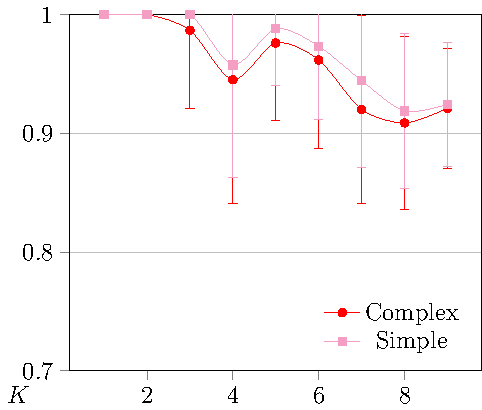
\includegraphics[width=.28\textwidth]{Figures/sec5_mlp_complexity_lime-figure2.pdf}%
                \label{subfig:decreasing_complexity_lime_recalls}%
            }\\
            \caption{Comparisons of results for our three metrics for SHAP (top row) and LIME (bottom row) explanations of equally accurate NNs with high and low complexity.}
            \label{fig:decreasing_complexity}
        \end{figure}
        
            To investigate this tradeoff, we compare SHAP and LIME explanations of two neural networks (NN) of differing complexity but nearly the same predictive performance. The first NN, $\mathcal{M}_1$, has 100 nodes in its hidden layer (the default in sklearn) and a test set AUC of about $.99$. The second, simpler NN $\mathcal{M}_2$, has only two nodes in its hidden layer and yet it also has a test set AUC of about $.98$. Figure \ref{fig:decreasing_complexity} visualizes our comparison of explanations of $\mathcal{M}_1$ and $\mathcal{M}_2$. %Additional results and further motivation for this strategy can be found in Appendix Section \ref{apx_sec:appendix_inconsistency}.

            We found that explanations by both SHAP and LIME of the simpler NN $\mathcal{M}_2$ were more data-aligned than explanations of the complex NN $\mathcal{M}_1$ in terms of each of our three metrics. %However, as shown by Figure \ref{fig:decreasing_complexity}, the improvements were marginal for the most part. \textcolor{red}{I don't think so. let's talk about it}. 
            For SHAP, we reject the null hypothesis of equal sign accuracies only for ``Age" with $p<001$ and ``Credit History" with a p-value of $0.04$. It is evident from Figure \ref{subfig:decreasing_complexity_shap_spearmans} that concordance did not rise significantly; we failed to reject the null hypothesis of equal concordances with a p-value of $.16$. Although relevance worsened for $k=8$ when explaining $\mathcal{M}_2$, the small improvements for $k=1,2,4,5,6,7$ were all statistically significant with $p<.001$ except for $k=4$, which had $p=.05$. % $6.21e-3$, $9.83e-4$, $4.73e-2$, $7.85e-5$, $9.73e-6$, and $8.17e-17$.
            For LIME, we could only conclude that the directionality of ``Married" improved by rejecting the null hypothesis of equal directionality with a p-value of $0.015$. However, the improvement to concordance was significant, as its test had $p<.001$. As for relevance, the results for $k=1$ were identical and the null hypothesis of equal relevance was rejected in favor of improvement for $k=2,6$ with p-values of $0.02$ and $0.01$. Overall, the results suggest that explanations of simpler models are more data-aligned than explanations of more complex models with equivalent predictive performance. 
            
            A reason that the explanations of the simple model $\mathcal{M}_2$ were better is that even though $\mathcal{M}_1$ and $\mathcal{M}_2$ may have similar behavior in how they generate training and test set label predictions, the additional expressive power of $\mathcal{M}_1$ allows the local behavior of its decision boundary to be more erratic. Given that SHAP and LIME are local function approximators, incorrect local behavior of $\mathcal{M}_1$ imposes a limitation on how data-aligned SHAP and LIME can be when explaining $\mathcal{M}_1$. 

            
       

        \subsubsection{Averaging Explanations of Different Models}
            The rate at which new machine learning models and methods appear has exploded, making it increasingly difficult for researchers to choose what model to use and ultimately explain.  Recent research on Rashomon sets \citep{semenova22rashomon,wang2022timbertrek,donnelly2023rashomon} finds that for a given dataset, there exist many models with similarly good performance. %Coupled with the fact that each of them has hyperparameters to tune, model selection is to a machine learning researcher as was finding a route \tw{ to the Spice Islands to Magellan (what?)}. 
            Therefore, a straightforward way to address concerns about what black box to explain is to train many models, explain each of them, and average the explanations. In this way, diverse information from the hypothesis space under consideration is included in the final (averaged) explanation. %Often, but depending on the dataset, many different models can be constructed that have nearly the same predictive performance \citep{semenova22rashomon}. Each nevertheless has a distinct decision boundary and captures different correlations in the data, and so post hoc explanations of those models can still differ.
            With this in mind, we repeat the experiments of Section \ref{sec:evaluating_faithfulness} twice, once with explanations of a single model and again with explanations constructed by averaging feature importance values over SHAP and LIME explanations of 10 unique NNs with ROC AUC at least $0.9$. The averaged explanations are constructed for SHAP and LIME separately and in the following manner. For each applicant, we obtain feature importance values in the prediction of that applicant's outcome by 10 NNs and then average the resulting importance 10 importance values for each feature together to get a final, averaged, feature importance vector. We seek to test if these averaged explanations improve over singular explanations with respect to data-alignment.
            % PUT THESE DETAILS IN APPENDIX
            %Each NN is trained with 5 hidden layers and for 10 iterations as before, but each NN initializes its training with a different random seed. We control for the inconsistency of the explainers by using default hyperparameters and keeping the random seed of the explainers the same. 
             
            This strategy showed some promise but the results of our Wilcoxon tests for improvement of data-alignment were not consistent between SHAP and LIME. The differences are visualized in Figure \ref{fig:mlp_increase}. 
             Regarding SHAP, Figures \ref{subfig:mlp_avg_shap_sign_accs} and Figure \ref{subfig:mlp_avg_shap_spearmans} show that there was a large improvement in directionality for ``Age" and small improvements in directionality for many other features. However, even with the mitigation, SHAP did have perfect directionality for as many features as LIME did.  It also had no discernible difference in concordance. 
            Showing a stark contrast with SHAP, LIME's directionality, concordance, and relevance were all significantly improved. We rejected the null hypothesis of equal sign accuracies in favor of improvement for ``Cosigner," ``Married," and ``Sex" with respective p-values of $0.04$, $4.56e-4$, and $2.87e-7$. Directionality for the other features was perfect for the other features both with and without the mitigation. We rejected the null hypothesis of equal concordances in favor of improvement as the p-value had $p<.001$. In contrast, there was no significant change to sign accuracy for any feature (all p-values were at least $0.15$) and no significant change to concordance, as we failed to reject the null hypothesis of equal concordances with a p-value of $0.25$.  Figure \ref{subfig:mlp_avg_lime_sign_accs} shows that LIME  had better directionality for ``Age," ``Cosigner," ``Married," and ``Sex." Given our results, we can only adduce that this strategy is effective for LIME. In particular, it was effective in increasing directionality and concordance, but not relevance.  %Our results are shown in Figure \ref{fig:mlp_increase}.
            
            %Figure \ref{subfig:mlp_avg_lime_spearmans} shows that LIME's averaged explanations had a slightly larger mean and slightly lower range while Figure \ref{subfig:mlp_avg_lime_spearmans} shows that concordance was almost unchanged for SHAP. Figures \ref{subfig:mlp_avg_lime_sign_accs} and  for LIME and \ref{subfig:mlp_avg_shap_sign_accs} and \ref{subfig:mlp_avg_shap_recalls} show that, with a few exceptions, the averaged explanations were at least as good as the explanations of a single model at identifying feature importance signs and the top-$k$ features. 
            
            %However, the strategy does not seem to be particularly beneficial for finding the top-$k$ features; the curves plotting the recall for SHAP and LIME in Figures \ref{subfig:mlp_avg_lime_recalls} and \ref{subfig:mlp_avg_shap_recalls} are nearly identical for the averaged and single explanation.%Figure \ref{fig:mlp_avg_recalls} also shows that the curves representing the relationships between $K$ and recall for $n=100$ bound the other curves from above. Therefore, this strategy appears to be effective in reducing both misalignment and inconsistency.

            % This strategy can be seen as a simplified version of \citep{donnelly2023rashomon}. Instead of leveraging explanations of good models trained on one dataset, they leverage explanations of optimal decision trees or GAMs trained on bootstraps of one dataset. At the time of writing, their method is not valid for more complex models like neural networks. It also produces statistics for feature importance instead of singular feature importance values. 
    

        \begin{figure}[t!]
            \subfloat[SHAP Directionality]{%
                \raisebox{.2cm}{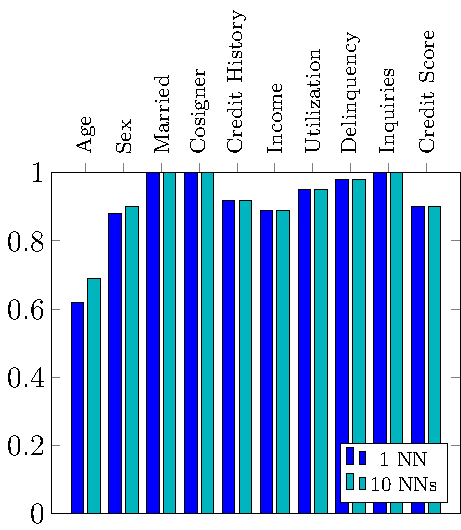
\includegraphics[width=.28\textwidth]{Figures/sec5_2_mlp_avg_shap-figure0.pdf}}%
                \label{subfig:mlp_avg_shap_sign_accs}%
            }\hspace{1cm}
            \subfloat[SHAP Concordance]{%
                \raisebox{.05cm}{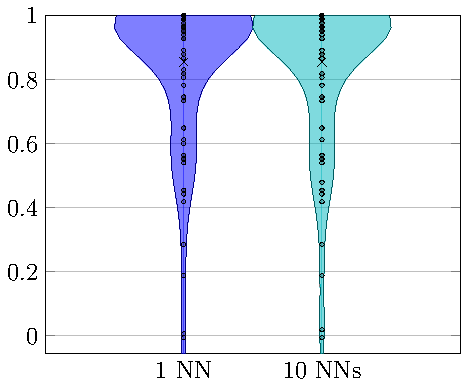
\includegraphics[width=.28\textwidth]{Figures/sec5_2_mlp_avg_shap-figure1.pdf}}%
                \label{subfig:mlp_avg_shap_spearmans}%
            }\hspace{1cm}
            \subfloat[SHAP Relevance]{%
                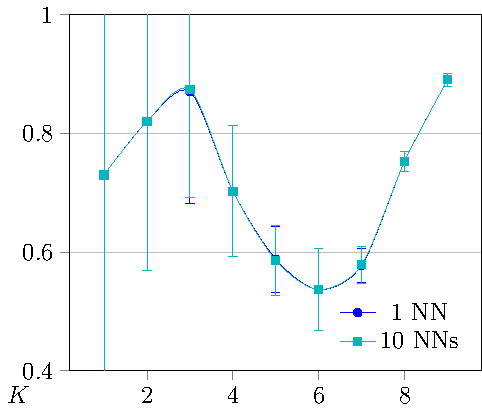
\includegraphics[width=.28\textwidth]{Figures/sec5_2_mlp_avg_shap-figure2.pdf}%
                \label{subfig:mlp_avg_shap_recalls}%
            }\\
            \subfloat[LIME Directionality]{%
                \raisebox{.2cm}{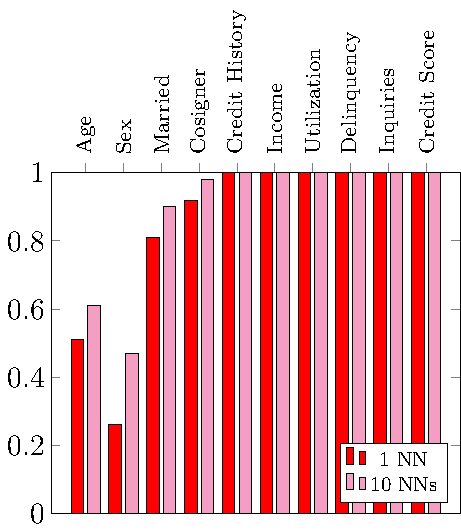
\includegraphics[width=.28\textwidth]{Figures/sec5_2_mlp_avg_lime-figure0.pdf}}%
                \label{subfig:mlp_avg_lime_sign_accs}%
            }\hspace{1cm}
            \subfloat[LIME Concordance]{%
                \raisebox{.05cm}{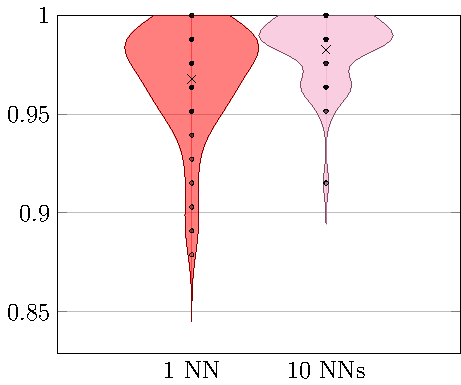
\includegraphics[width=.28\textwidth]{Figures/sec5_2_mlp_avg_lime-figure1.pdf}}%
                \label{subfig:mlp_avg_lime_spearmans}%
            }\hspace{1cm}
            \subfloat[LIME Relevance]{%
                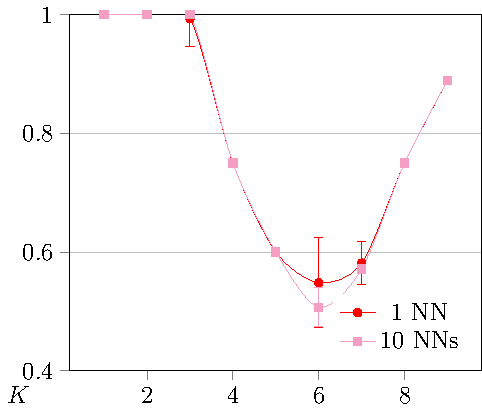
\includegraphics[width=.28\textwidth]{Figures/sec5_2_mlp_avg_lime-figure2.pdf}%
                \label{subfig:mlp_avg_lime_recalls}%
            }\\
            \caption{Comparisons of data alignment for SHAP (top row) and LIME (bottom row) explanations of 1 NN versus explanations constructed by averaging the feature importance values of 10 NNs.}
            \label{fig:mlp_increase}
        \end{figure}
        

   
    
    \subsection{Summary and Discussion of Mitigation Strategies}
            \label{sec:summary_and_strategies}
             The main results of our mitigation experiments are that when using SHAP the Shapley values should be normalized, and when using LIME, it may be worthwhile to aggregate the explanations of many LIMEs, and individual LIME explainers should have large $\nu$ and $n$. Secondarily, it is recommended to seek black boxes that optimize the trade-off between complexity and predictive power and to average explanations over ensembles of explainers and/or models. 
            %It makes less sense to combine explanations of a single model than explanations of multiple models because of the idea that ``all models are wrong". 

            We discuss two unsuccessful mitigation strategies in the Appendix, both based on aggregating explanations of a single black box. The first exchanges simple averaging for a method of ranked choice voting known as the Borda Count and the second averages SHAP and LIME explanations together. We believe that a core reason why these two strategies were unsuccessful is because they only involve a single black box model. Finding common (valid) patterns within multiple black boxes is possible by aggregating explanations of those models, whereas aggregations of explanations of a single black box can at best reveal the single, imperfect, pattern identified by that black box. Ignoring bias and error in the dataset, each explanation has two layers of approximation error with respect to the ground truth, whereas each black box has only its own approximation error and captures different patterns in the training data. Thus, researchers may find averaging feature importance values obtained by many models both a useful and intuitive strategy \citep{dong2020variable,donnelly2023rashomon}.  %With the configuration of data and model we used, the local error rates of both SHAP and LIME were skewed to the right, implying that the mean local fidelity over samples of SHAP and LIME models can decrease as the sample size increases. However, it is difficult to validate this claim because the local fidelity of SHAP and LIME is not an especially good measure of how faithful their explanations are to $\mathcal{G}$. That averaging SHAP and LIME together did not yield a consistent and substantial advantage is likely due to the simplicity of the technique. For this reason, we suggest that more research be done on this topic. 
            
            Researchers who would like to investigate the importance and impact of features in the data  process may find exploring the following general strategy useful.
        %First, the choice of explainer(s) used for the strategy should be guided by user preference for the types of feature importance outlined in Section \ref{sec:theoretical_considerations}. For example, LIME should be preferred to SHAP if  $\boldsymbol{\beta}$ is considered to be the ground truth feature importance representation.  %construct average explanations over a collection of good LIME explanations of good models. If situational importance is more suitable than theoretical importance for the application, researchers should instead average over SHAP explanations of good models. 
            When starting the prediction stage, the dataset should be pre-processed to remove highly correlated features\footnote{If possible, adjustments can be made to account for confounding. Tools like E-values\citep{gaster2023quantifying} and Pearl's backdoor criterion can be used for this purpose.}. % The causal graph can be estimated using Bayesian Networks if sufficient domain knowledge is available.}
            Having pre-processed the data, researchers are encouraged to train $B\geq 1$ black box models with simple enough decision boundaries to not lose too much predictive performance compared to more complex models \footnote{Ideally, Rashomon sets of models would be constructed and the simplest models in them would be collected. However, at the time of writing, this is only possible for decision trees and GAMs.}. To construct a more robust explanation of a model's predicted outcome for an instance, the results of multiple explainers of that model can be aggregated by, e.g., averaging the feature importance values for each feature over the explainers. An even more robust final explanation for an instance can be produced by averaging over the importance values given in the $B\times E$ explanations of the predictions of $B$ models by $E$ explainers.
          


\subsection{Case Study Using Real Data and Econometric Method}
    \label{sec:case_study}
    To validate the efficacy of our mitigation strategies and illustrate how they could be employed in practice, we test whether they give an advantage over default usage of SHAP and LIME in extracting the same marginal effects as those found in an econometric paper on the approval of home loan applications \citep{bane2006econometric}. In particular, we will tailor the framework outlined in Section \ref{sec:summary_and_strategies} to form mitigated pipelines for SHAP and LIME separately. The results of these mitigated pipelines will be compared to default usage of SHAP and LIME. The home loan dataset is publicly available and originates from a study by the Federal Reserve Bank of Boston \citep{hunter1996cultural}. We take the ground truth $\boldsymbol{\beta}$ to be the coefficients of the logistic regression model obtained in the analysis of \cite{bane2006econometric} on that dataset. This is justifiable because econometric modeling is equipped to capture $\boldsymbol{\beta}$. The linear ground truth model derived from their logistic regression model appears in Equation (\ref{eqn:econ_gt}). The meanings and ranges of each feature appear in the Appendix.  %We will use the logistic regression coefficients to evaluate SHAP and LIME explanations in the same manner as has been done throughout this paper. We suppose that the logistic regression coefficients have the correct signs and magnitudes relative to each other, not that the logistic regression itself is the true causal model underlying home loan approvals in Boston. 

    %\begin{tcolorbox}[title = Econometric Ground Truth Model $\mathcal{G}$]
    \begin{equation}
    \label{eqn:econ_gt}
    \begin{split}
        \mathcal{G}(X) =.8 + 3.5\cdot \text{good credit} + 4.7\cdot \text{purchaser type} -4.4 \cdot \text{PMI approved} - .4 \cdot \text{multi family} \\ -2.5 \cdot \text{unver} + .9 \cdot \text{fixed rate} - 1.4 \cdot \text{bankruptcy} - .9 \cdot \text{value rate} - .03 \cdot \text{debt rate} \\- .7 \cdot \text{old} + .8 \cdot \text{married} - .8 \cdot \text{gift}
    \end{split}
    \end{equation}
    %\end{tcolorbox}
    %\subsection{Baseline Performance}
    %Figure \ref{fig:econ_cmp} compares the explanation quality  for 100 applicants from the baseline pipeline and recommended pipeline. %In the Appendix, we show also compare results for importance sign accuracy, Spearman rank correlation, and recall.
    

    Our mitigated pipelines for SHAP and LIME are applications of the mitigation framework outlined in Section \ref{sec:summary_and_strategies}. First, we split the dataset into 80\% training data and 20\% testing data. Then we produce $B=10$ NNs with test set AUC that are at least $.9$. These $10$ NNs are selected from a family $210$ of NNs that we trained. The family of NNs used a parameter grid consisting of $2,5,10,\ldots,100$ hidden layer nodes and random seeds $1,2,3,\ldots,10$. We selected the 10 NNs which had the fewest numbers of hidden layer nodes and test set AUC that was at most $\epsilon=.02$ less than the highest test set AUC achieved within the family of NNs. and produce $E=10$ SHAP and LIME explainers for each NN. The mitigated LIME pipeline uses all $B=10$ NNs and $E=10$ LIME explainers for each NN. Each LIME explainer has $\nu=n=10000$. Because SHAP is  deterministic and the NN averaging strategy did not significantly increase directionality and concordance for SHAP, we use $B=E=1$ and normalize the Shapley values. Baseline explanations come from explanations of one NN with accuracy $.86$, ROC AUC $.93$ with individual SHAP and LIME explainers both using default settings. 


    Both the SHAP and LIME variants of our general strategy generally had results which improved upon the baseline in at least one respect. The improvements can be seen in Figure \ref{fig:econ_cmp}. Indeed, our strategy applied to SHAP significantly improved directionality for all features except two (``gldin" and "gift") and significantly improved both concordance and relevance.  Our strategy applied to LIME significantly improved concordance overall, improved directionality greatly for ``fixadj," and ``gift," and significantly improved relevance for the top 2, 3, and 4 features. %It had worse directionality only for ``vr" and ``obrat," and worse relevance for features not in the top-4. 

    %%\textcolor{red}{what are the econometric insight? we might have been overclaiming}
    %Figure \ref{fig:econ_cmp} visualizes the results. The directionality values from our recommended strategy with SHAP and LIME were at least as good as those from the baseline for all features except ``pubrec" (bankruptcy filed) for LIME and ``vr" (value rate) for SHAP (see Figures \ref{subfig:econ_lime_sign_accs} and \ref{subfig:econ_shap_sign_accs}). The concordance plots for both SHAP and LIME in Figures \ref{subfig:econ_shap_spearmans} and \ref{subfig:econ_lime_spearmans} show that the recommended pipeline rankings were generally more faithful than the most faithful explanations from the equivalent baseline. Finally, it can be seen from Figures \ref{subfig:econ_lime_recalls} and \ref{subfig:econ_shap_recalls} that the recommended strategies using SHAP and LIME both have substantially higher relevance for all $k\neq 1,\ 10,\ 11$.
     
% \begin{figure}[!h]
% \centering
%     \begin{subfigure}[t]{0.28\textwidth}
%     \centering
%     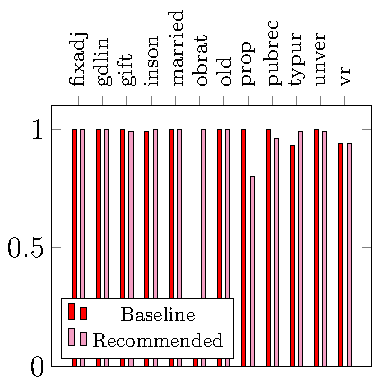
\includegraphics[width=\textwidth]{Figs/econ_cmp-figure0.pdf}
%     \caption{Directionality} \label{fig:econ_cmp_sign_accs}
% \end{subfigure}\hspace{1cm}
% \begin{subfigure}[t]{0.28\textwidth}
%     \centering
%     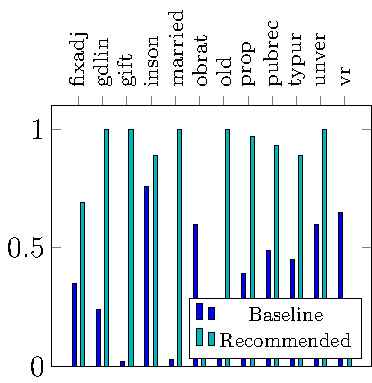
\includegraphics[width=\textwidth]{Figs/econ_cmp-figure1.pdf}
%     \caption{Relevance} \label{fig:econ_cmp_spearmans}
% \end{subfigure}\hspace{1cm}
%  \begin{subfigure}[t]{0.28\textwidth}
%     \centering
%     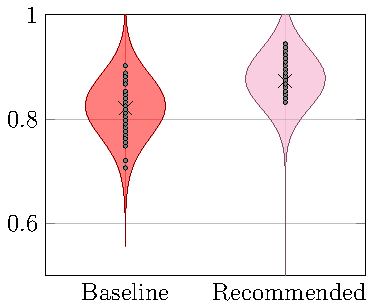
\includegraphics[width=\textwidth]{Figs/econ_cmp-figure2.pdf}
%     \caption{Recall}
%     \label{fig:econ_cmp_recalls}
% \end{subfigure}
% \caption{Improvements due to use of recommended pipeline instead of one without any of our mitigation strategies}\label{fig:econ_cmp}
% \end{figure}


        \begin{figure}[t!]
            \subfloat[SHAP Directionality]{%
                \raisebox{.2cm}{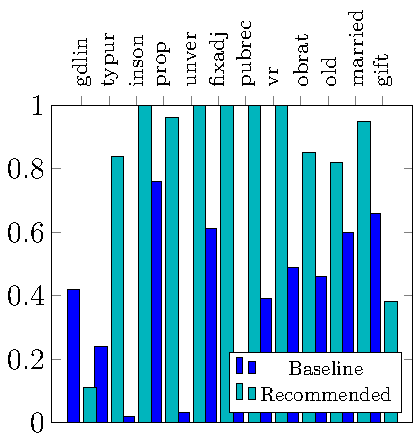
\includegraphics[width=.28\textwidth]{Figures/shap_econ-figure0.pdf}}%
                \label{subfig:econ_shap_sign_accs}%
            }\hspace{1cm}
            \subfloat[SHAP Concordance]{%
                \raisebox{.05cm}{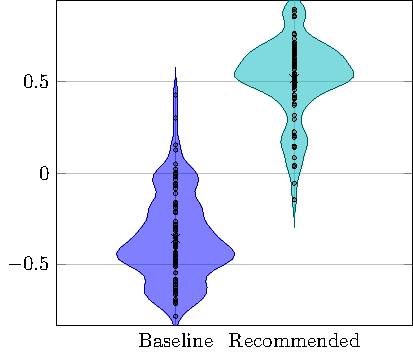
\includegraphics[width=.28\textwidth]{Figures/shap_econ-figure1.pdf}}%
                \label{subfig:econ_shap_spearmans}%
            }\hspace{1cm}
            \subfloat[SHAP Relevance]{%
                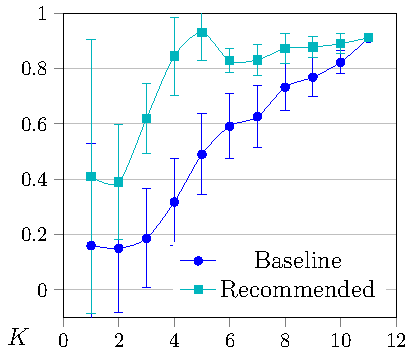
\includegraphics[width=.28\textwidth]{Figures/shap_econ-figure2.pdf}%
                \label{subfig:econ_shap_recalls}%
            }\\
            \subfloat[LIME Directionality]{%
                \raisebox{.2cm}{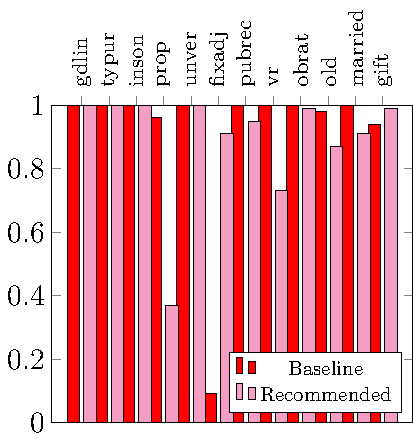
\includegraphics[width=.28\textwidth]{Figures/lime_econ-figure0.pdf}}%
                \label{subfig:econ_lime_sign_accs}%
            }\hspace{1cm}
            \subfloat[LIME Concordance]{%
                \raisebox{.05cm}{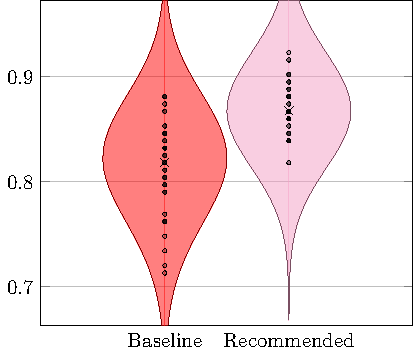
\includegraphics[width=.28\textwidth]{Figures/lime_econ-figure1.pdf}}%
                \label{subfig:econ_lime_spearmans}%
            }\hspace{1cm}
            \subfloat[LIME Relevance]{%
                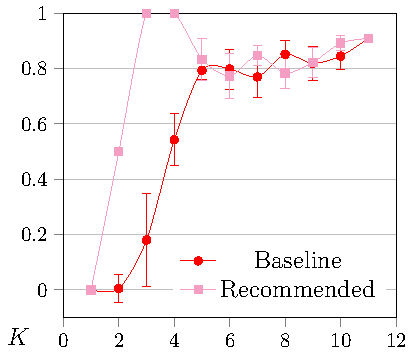
\includegraphics[width=.28\textwidth]{Figures/lime_econ-figure2.pdf}%
                \label{subfig:econ_lime_recalls}%
            }\\
            \caption{Improvements due to use of recommended pipeline instead of one without any of our mitigation strategies}\label{fig:econ_cmp}
        \end{figure}
    %\tw{Figure 12 (f) makes our strategies less convincing. The result looks weird. Did you double check?}



\section{Discussion and Conclusion}
    \label{sec:discussion}
    As post hoc explanations are gaining popularity in business research, we found an alarming trend of using them to make claims about the marginal effects of variables in the data. In our survey of 150 business papers, we found 42\% of papers use LIME or SHAP for this purpose. However, the validity of this use of post hoc explanations has not been studied in the literature. 
    This paper is the first effort towards this purpose. 
     In the following sections, we will summarize our findings and give some parting advice for the use of post hoc explainers for obtaining data insights in business research. 
    We also contribute to the business literature by proposing some simple and intuitive mitigation strategies which we found to benefit explainer data-alignment to varying extents.
    %    
    %In this paper we have introduced and investigated issues of misalignment and inconsistency of post hoc explanations. Our thorough literature review uncovered that business researchers using post hoc explanations value data-alignment. Thus we have contributed to the business literature by providing both theoretical and empirical evidence that the two most popular explainers, LIME and SHAP, often produce misaligned explanations. Notably, we proved that SHAP is inherently unsuitable to infer information about $\boldsymbol{\beta}$. %We have also identified various factors that contribute to misalignment and inconsistency. 


    \subsection{Main Findings}
        Our paper contributes several important findings to the use of post hoc explanations in business research.

            First, through an extensive literature review, we found that the use of post hoc explanations to infer information about the data is quite prevalent. In the 150 papers we reviewed, 63 used SHAP or LIME to draw conclusions about the $X\rightarrow Y$ relationship instead of the $\mathcal{M}(X)\rightarrow \hat{Y}$ relationship. Such use deviates from the intended purpose of post hoc explainers: they are designed to explain the machine learning model, not to infer any information from the data. Identifying this misuse of post hoc explanations is an important contribution of this paper. Note that while post hoc explanations have been first introduced and widely used in the machine learning community, the issue we discuss in this paper is less of a concern for that community because computer scientists are more interested in explaining the machine learning models. Post hoc explainers are used by them to understand a model's behavior in order to diagnose and debug the model. However, the goal of business researchers is to understand the data and the underlying phenomena, making this issue more prominent in business research.
        % Using simulated loan application datasets, we produced ground truth application approval mechanisms $\mathcal{G}$ along with NN approximators $\mathcal{M}$ trained on $\mathcal{G}$ and investigated how well popular post hoc explainers could recover the $\boldsymbol{\beta}$ underlying $\mathcal{G}$. This investigation was motivated by the need to assess the utility of post hoc explainers to business researchers and managers. We used our results from the investigation using simulated data to propose a set of mitigations that would worth exploring in practice. Finally, we tested the efficacy of this set of mitigations in a test to see if we could use LIME to reproduce the results of an econometric study of home loan applications. We found that although it was far better to use them than not, the resulting explanations were still imperfect. 

        % When evaluating the ability of the two most popular post hoc explainers, SHAP and LIME, to extract faithful insights from both real and simulated data, we identified the following issues that are cause for concern for researchers interested in $\boldsymbol{\beta}$ estimation problems using post hoc explainers. 

       Second, we provide both theoretical and empirical evidence that SHAP and LIME explanations are, in fact, not data-aligned. In our investigation, we discovered that SHAP and LIME incorrectly represent the signs and relative importance of the marginal effects of the explanatory variables. As shown in Section \ref{sec:causes_of_misalignment}, SHAP and LIME tend to be data-misaligned even in scenarios where they explain an accurate machine learning model trained on data whose features are mutually independent and whose target is derived from a simple linear ground truth model - scenarios which are, in a sense, ideal. This observation suggests a need for caution when interpreting variable relationships based on post hoc explanations. It opens up a dialogue about the complexities of deriving accurate insights from machine learning models via post hoc explainers, contributing to a deeper understanding of their limitations and paving the way for future research in this area. In light of these insights, it may be beneficial for the academic community to revisit prior analyses that have relied heavily on post hoc explanations. This reassessment could ensure that interpretations and conclusions drawn from such models are robust and reflective of their underlying dynamics. Our findings underscore the importance of continuous critical evaluation in the field, especially as we seek to refine our understanding and application of these explanatory tools. %Our finding is echoed in other recent studies that compared the  \cite{baghdasaryan2021comparison}
        
        Third, we find that the reason for the data-alignment is different for SHAP and LIME. Achieving data-alignment using SHAP feature importance values is inherently impossible due to the nature of Shapley values. Shapley values represent a feature's contribution to a prediction by considering not only the feature's marginal effect but also its value and the influence of other variables within the explanation process. In the particular case where SHAP explains a linear model, the vector of Shapley values is given by $\boldsymbol{\beta}(\boldsymbol{\xi}-\bar{\mathbf{x}})$, diverging from a direct representation of $\boldsymbol{\beta}$. Conversely, LIME's data-misalignment arises from the mechanics of its default ridge regression approach. Our analysis, supported by Theorem \ref{thm:lime_thm}, indicates that LIME could achieve data-alignment by avoiding the discretization of numerical inputs, sampling many points for its synthetic regression problem, and opting for a significantly larger bandwidth than the default. Yet, even with these adjustments, common properties of real-world data such as correlated variables often hinder the attainment of data-alignment. Nonetheless, it is noteworthy that our evaluations generally reveal \textit{LIME to provide explanations more aligned with the ground truth compared to SHAP}.
 
        
         Finally, we identify several mitigation strategies that show promise in enhancing the data-alignment of explanations across various stages of the explanation pipeline. These strategies, validated through empirical testing, offer significant improvements in aligning explanations more closely with marginal effects. However, it is important to acknowledge that none of the strategies can guarantee complete congruence with marginal effects. This absence of a full guarantee means that while explanations may sometimes align closely with the marginal effects, they cannot reliably do so. Such a scenario potentially restricts the applicability of post hoc explanations, as users may remain uncertain about the extent to which these explanations accurately mirror the underlying the marginal effect structure. This limitation underscores the need for cautious interpretation and application of post hoc explanation methods in practical scenarios.
        
        
        % \textcolor{red}{what else did we *find*?}

            
        % Second, users must deal with inconsistent explanations because not only do e.g. SHAP and LIME each produce different explanations for the same outcome, but LIME may produce self-contradictory explanations of the same outcome. How to select an explanation(s) from the myriad available from different combinations of accurate black box models, explainers, and explainer hyperparameters is up to the user, but the mitigations suggested in this paper can help users make more informed decisions.%but robustness checks like those presented in this paper can be used to estimate how confident users can be in their selection(s). 



        % stuff re: prescriptive removed
        %Our main finding regarding prescriptive insights is that LIME, SHAP, and DiCE seem to only be of use for actionable recourse a minority of the time. When tasked with generating new application profiles for denied loan applicants, those new application profiles would be approved by $\mathcal{G}$ less than 50\% of the time. %\textcolor{blue}{May need to be removed!! We showed that... DiCE, a counterfactual explainer (as opposed to an attributive one like SHAP and LIME) was always able to produce new application profiles for rejected loan applicants that would lead to approval in our experiments (for a sufficiently small sparsity parameter). }For DiCE, if we restrict the range of feature variations (within one standard deviation) and the number of features allowed to vary, it can only provide prescriptive insights to a small number of denied applicants.
        
    % \subsection{On Mitigation Strategies}
    %     We proposed some intuitive mitigation strategies for the issues of unfaithful and inconsistent explanations. Each of them was effective with respect to at least one of our three metrics. However, none of them were fully effective solutions that would guarantee that practitioners could confidently use LIME or SHAP for $\boldsymbol{\beta}$ estimation and econometric modeling. Thus, we encourage cautionary usage of SHAP and LIME and to consider exploring the usage of our mitigation strategies in efforts to obtain more data-aligned explanations. 
        
    %     Our principal finding regarding faithfulness was that SHAP has no chance at data-alignment unless its Shapley values are normalized by the difference between feature values and feature means. We also found that the most important strategy for increasing the faithfulness of LIME is to disable discretization of numerical features and to make the number of samples and kernel bandwidth it uses for weighted ridge regression large. 
        
    %     %We found some success in increasing the faithfulness of an explanation of a model $\mathcal{M}$ to the ground truth $\mathcal{G}$. As expected, whether $\mathcal{M}$ and $\mathcal{E}$ can correctly predict decisions from $\mathcal{G}$ affects how faithful their explanations are to $\mathcal{G}$. In addition to ensuring low generalization error of $\mathcal{M}$, we also noted that ensuring that $\mathcal{M}$'s training data without correlated or confounded features resulted in remarkably better results than otherwise. However, it is important to note that the explanations were still usually imperfect even though the model and data were ideal. 
    
    %     To combat inconsistency, we proposed techniques to construct aggregate explanations that are better on average than individual explanations. These strategies worked by  averaging feature importance values obtained from explanations obtained from different combinations of models and explainers. The motivation behind these averaging strategies was that they address uncertainty in the choices users need to make by aggregating the many combinations of models and explainers that are the root of the uncertainty. In addition to addressing inconsistency, these strategies resulted in statistically significant improvements in at least directionality, concordance, or relevance. 

    %     In exploring mitigation strategies, we did not find evidence that LIME or SHAP can be used in a way that makes them suitable alternatives to traditional econometric modeling. Although our recommended strategies for SHAP and LIME compared favorably to their associated baselines in a test to reproduce results an actual econometric study of loan approval, they were unable to consistently extract the $\boldsymbol{\beta}$ that the econometricians found. 

%\textcolor{red}{add in the discussion that althgouh we do not know when the explanation aligns with beta, we can identify when they do not: just run  pipeline multiple times with different split of data and different ML model, if the results do not agree, it is a clear sign that the beta-alignment is low}
    
    
    \subsection{On the Use of Post Hoc Explanations}
  We want to emphasize that this paper focuses on the issue of using post hoc explanations to make inferences about the data. We do not explore their use in explaining the machine learning model $\mM$ or its predictions $\mathcal{M}(X)$, which is the primary intended purpose of post hoc explainers. However, it is important to note that even this intended use of post hoc explainers is controversial \citep{garreau2020looking,alvarez18robustness,kumar20shap,jacovi2023diagnosing}. For the scope of this paper, our discussion is solely focused on inferring ground truth information from $\mathcal{G}$ through the explanations for $\mathcal{M}$.

    \subsubsection{General Usage}
      While this paper recommends against using post hoc explanations to make any definite claims about data, it does not mean that post hoc explanations cannot be used at all. Instead of using them as a tool to \textbf{validate} hypotheses and viewing the explanations as evidence, we propose to use post hoc explanations to \textbf{propose} hypotheses that can guide subsequent efforts after they are corroborated.  %\tw{As a preliminary step, researchers can use the level of inconsistency between explanations of models trained on different splits of the data to gauge data-alignment, viewing explanations which do not share common patterns found the collection of explanations as an indication of its implausibility. Following the preliminary step, a
      %An ideal usage of a hypothesis which is deemed to be plausible and interesting would be to empirically validate it through e.g. randomized trials and with collaboration with domain experts. %(1. don't mention inconsistency. just say first use post-hoc explanaitons to propose some hypothesis. While they do not guarantee 100\% accuracy, they do offer a high probability of recovering the true effect in the data. Then use follow-up analysis. Don't only say random trials or domain experts. They could use other causal analysis such as (I'll ask Jeffrey about this)}If this were not presently feasible, researchers could at least call on domain experts to validate the hypothesis \citep{donnelly2023rashomon} or do 
     Further analyses are necessary because hypotheses produced by explainers are not guaranteed to be correct, and can be performed using tools which are more suited to ascertain causal relationships. For example,  \cite{zhang2023can} follows up their search for important features for restaurant survival using SHAP by using causal forests to estimate the treatment effects of those features. Similarly, \cite{hanauer22boosting} use traditional regression as a trusted baseline that they compare SHAP explanations to. 
%      Additionally, as was done in \cite{tang2024china}, plausible post hoc explanations can be used to aid classical regression analyses as a feature selection method. That is, researchers can opt to use only those features which are said to be important by a post hoc explainer(s) in their regressions but should keep in mind that those features may not actually be important to $\mathcal{G}$. \textcolor{red}{I think this is controversial. This is relevance and we said relevance is not 100\%}
    
    
    
% \textbf{How to Make Fruitful use of post hoc Explainers}.
% \cite{Usc paper and the other paper using shap to select features}
%  Model-agnostic post hoc explainers certainly have legitimate use cases, but due to the nature of real business datasets and stakes associated with business problems, we urge the business community to use them with caution and with tempered expectations. The problems of data-misalignment and inconsistency make it difficult for researchers to choose explanations in a principled fashion and ascertain their truth value. Thus, without sufficient domain knowledge or evidence, a researcher can neither believe nor trust the content of a post hoc explanation, nor use it to make inductive inferences. In such a context, the only truly principled view of a post hoc explanation is as a hypothesis. 
 

    
    %Then their explanations can be used as a basis for more rigorous analysis. For example, the treatment effects of features identified as important by the explainers can be estimated using causal forests \citep{zhang2023can}.   
    
        %The outline given in Section \ref{sec:summary_and_strategies} can undoubtably be improved and tailored to user-specific situations, and so is worth expounding. We do so below, and provide additional information that could be useful in different use-cases. 


        %During Prediction stage, before even beginning model development, users should use correlation analysis and any available domain knowledge to identify correlated or colinear features, and then decide whether to drop them from the dataset. % attempt to understand the causal graph associated with their problems and employ statistical tests of unconfoundedness assumptions. With this knowledge, users need to decide whether it is worthwhile to use post hoc explainers instead of randomized experiments. If so, the data should be pre-processed to have the desirable properties we have outlined previously. Domain knowledge and knowledge of the causal graph are useful for this purpose~\citep{zhao2021causal}.% to remove redundant features, causal descendants of a collinear pairs of causally linked features. Confounders should be controlled for if possible.
        %Then, unless users are only interested in explaining a particular black box model, we propose that many be generated and used for explanations. This is due to the Rashomon Effect\citep{semenova22rashomon}, which states that models (interpretable or otherwise) with approximately the same predictive performance will represent different relationships of the input features to the target. In other words, equally good models will have different (possibly conflicting) explanations and interpretations. In the best case, users could leverage explanations entire Rashomon sets of good models from specified model classes and training datasets. We showed that this technique was useful when averaging explanations over a rather small set of NNs with high ROC AUC using LIME explainers which correctly classify the input being explained. Additionally, because we found that the complexity and generalization error of $\mathcal{M}$ was related to post hoc explanation quality and variability, we propose that researchers gather as much training data as feasible.%.qasw11111 and take care not to overfit their models. %Overfitting is especially detrimental because the complexity of the decision boundary of $\mathcal{M}$ contributes to the instability of the explainer. After all, even a perfect explainer for a model which is highly locally nonlinear must be unstable. Thus, needless complexity in a decision boundary due to overfitting could cause an explainer of the decision function to be unstable when it should not be.  

       
        %When starting the explanation stage, users should keep in mind that post hoc explanation can be accidentally misused due to a fundamental misunderstanding of the explainer. For example, \cite{kaur2020interpreting} showed that practitioners misused explanations due to having an incorrect understanding of Shapley values. \cite{jacovi2023diagnosing} also discusses the possibility of users coming away with an incorrect understanding of incomplete explanations because they fill in missing information with their own biases. Users should ensure that they have a complete understanding of how explainers they intend to use work and how their biases may affect their understanding of the explanation. Having done this, we recommend researchers to view post hoc explanations simply as hypotheses and avoid using them to assert novel findings about $\mathcal{G}$ or claiming that they confirm existing hypotheses. 
        
        %As we have discussed, due to the problems of misalignment and inconsistency, researchers should not trust that a single explanation from any explainer applied to any black box model is true unless they can corroborate the explanation. Ideally, explanations would be corroborated using domain knowledge. Otherwise, users could consider comparing the explanations with patterns found in inherently interpretable models or use explainers only for exploratory analyses that are followed up with more rigorous analysis. For example, we recommend that researchers use robustness checks to figure out how confident they can be in the variability of explanations, and select or aggregate explanations from among the large set of explanations created during the robustness checks. 

\subsubsection{Can SHAP be Used as an Alternative to Econometrics Methods?}
    We discuss whether SHAP can be used as an alternative to traditional econometric modeling because this type of usage was a pattern we found in our literature review. That is, researchers were motivated to use SHAP explanations of an ML model to obtain feature importance values because of perceived advantages XAI has over regression analysis. The most commonly cited advantage is that, unlike traditional least squares regression methods, SHAP explanations automatically include nonlinearities and interactions \cite{hanauer22boosting,berger2023supply,srivastava23energy,banulescu2023practical,li24roles}. For example, \cite{berger2023supply} describes their motivation to use SHAP by asserting that SHAP can provide similar economic insights to pooled OLS \emph{and} capture the non-linear impacts of features. \cite{srivastava23energy}, which expresses the desire to use and explain ML models with SHAP in order to find factors driving energy consumption because ML models can ``detect highly complex interactions between drivers of energy consumption", is an example of this. Furthermore, \cite{zhou23consumption} says that XAI methodology is appealing because it does not necessitate ``...the construction of more intermediate variables and complex statistical analysis". Similarly, \cite{banulescu2023practical} are drawn away from logistic regression because it suffers when a large number of predictors are used. \cite{hanauer22boosting} choose not to use traditional linear regression analysis used for fundamental stock analysis and instead explain random forest and XGBoost models because the ML models deal with non-linearities, interactions, and noisy features. \cite{li24roles} makes inferences about bike sharing by explaining their XGBoost model instead of examining the coefficients of their linear regression because the XGBoost had better predictive performance. 

     The fact that SHAP is a local explainer makes its use for obtaining global feature importance unnatural, and this is a shortcoming SHAP has in comparison to econometric modeling. We found that authors often circumvented SHAP's status as a local explainer by computing the average of the absolute Shapley values over their test set and using the results as measures of global feature importance. \cite{lenaers23rent,maeng23vr,guenther2023useful} are all examples. This obviously comes at a cost of losing any indication of the directionality of impact by features. However, they must do this because the means of signed Shapley values should be 0 due to Equation \ref{eqn:shap_gt}. This is usually the case empirically; \cite{lenaers23rent,maeng23vr,jiang24churn} all show scatter plots of the signed Shapley values of each feature over their dataset and the empirical distributions of the Shapley values are almost always centered at 0. Equation \ref{eqn:shap_gt} implies that the expected absolute Shapley value for feature $X_j$ is proportional to $\beta_j$, but also a function of the mean and standard deviation of $X_j$. So, unless all of the $X_j$ are identically distributed, the expected absolute Shapley values may not be comparable for the sake of relative importance in the same way as the $\beta_j$. In other words, a ranking of the average absolute Shapley values may be different than the ranking of the $\mid \beta_j\mid$.  %For example, if $\beta_1=1$ and $\beta_2=2$ with $X_1\sim\mathcal{N}(\mu_1=100,\sigma_1=1)$ and $X_2\sim \mathcal{N}(\mu_2=0,\sigma_2=\frac{1}{10})$ that are viewed as important in the sense of the effect of a unit increase, the expected absolute Shapley value for $X_1$ is larger than the expected absolute Shapley value of $X_2$ even though $X_2$ is more important than $X_1$ because $\beta_2>\beta_1$:
    % \begin{equation*}
    %     \mathds{E}[\mid \beta_1(X_1-\mu_1)\mid] = \sqrt{\frac{2}{\pi}} > \mathds{E}[\mid \beta_2(X_2-\mu_2)] = \frac{1}{5}\sqrt{\frac{2}{\pi}}
    % \end{equation*}

\subsection{Final Remarks}% and Future Work}
This paper aims to highlight the issue with a rising use of post hoc explanations that we identify as inappropriate. To demonstrate the seriousness of this problem, we show that the misalignment occurs even in the simplest context, where the ground truth $\mathcal{G}$ is linear and features are  independent. Even in this simple case, SHAP and LIME produce misaligned explanations and the quality becomes worse as the feature dimension increases. We expect that in more realistic scenarios their performance can only be worse. Real decision processes are often non-linear and involve feature interactions and unobservable features; naturally, these added complexities should reduce the efficacy of SHAP and LIME, making it even more challenging to obtain data-aligned explanations. Given the uncertainty regarding the validity of post hoc explanations, researchers should view them skeptically and consider them as hypotheses rather than definitive claims about reality. 

%\tw{should Figure 13 be updated since we are in the middle of 2024 and there should be more papers in 2024} That is the updated version. 
 
 % When feasible, we advocate for intrinsically interpretable models to be used instead. %When data have unobserved confounders, randomized experiments should be used to identify treatment effects.


    % reword to remove word MISUSE; need to say instead that users get incorrect misunderstanding
    %Throughout this paper, we have shown how and why the use of post hoc explainers could lead to confusion for business researchers and bad decision making for businesses. Our experiments demonstrated SHAP and LIME's inability to produce consistent and faithful explanations. Possible consequences of this include businesses or customers trying to improve upon some outcome, which could waste time and resources by adjusting for an irrelevant feature that LIME or SHAP implied was important, or even worsen the outcome they were trying to improve. On the surface, model-agnostic post hoc explainers are attractive because they are easy to use and applicable to any model with any dataset. However, their propensity toward unfaithful and / or inconsistent explanations decreases their efficacy. Due to the stakes involved with understanding business problems, post hoc explainers should only be used with great caution. 
        

% Acknowledgments here
\ACKNOWLEDGMENT{The authors gratefully acknowledge the existence of
the Journal of Irreproducible Results and the support of the Society
for the Preservation of Inane Research.}


% References here (outcomment the appropriate case)

% CASE 1: BiBTeX used to constantly update the references
%   (while the paper is being written).
%\bibliographystyle{informs2014} % outcomment this and next line in Case 1
%\bibliography{<your bib file(s)>} % if more than one, comma separated

% CASE 2: BiBTeX used to generate mypaper.bbl (to be further fine tuned)
%\input{mypaper.bbl} % outcomment this line in Case 2

%If you don't use BiBTex, you can manually itemize references as shown below.


\bibliographystyle{informs2014}
\bibliography{refs}

\newpage


\end{document}
% %%%%%%%%%%%%%%%%%?